\documentclass[twoside]{book}

% Packages required by doxygen
\usepackage{fixltx2e}
\usepackage{calc}
\usepackage{doxygen}
\usepackage[export]{adjustbox} % also loads graphicx
\usepackage{graphicx}
\usepackage[utf8]{inputenc}
\usepackage{makeidx}
\usepackage{multicol}
\usepackage{multirow}
\PassOptionsToPackage{warn}{textcomp}
\usepackage{textcomp}
\usepackage[nointegrals]{wasysym}
\usepackage[table]{xcolor}

% Font selection
\usepackage[T1]{fontenc}
\usepackage[scaled=.90]{helvet}
\usepackage{courier}
\usepackage{amssymb}
\usepackage{sectsty}
\renewcommand{\familydefault}{\sfdefault}
\allsectionsfont{%
  \fontseries{bc}\selectfont%
  \color{darkgray}%
}
\renewcommand{\DoxyLabelFont}{%
  \fontseries{bc}\selectfont%
  \color{darkgray}%
}
\newcommand{\+}{\discretionary{\mbox{\scriptsize$\hookleftarrow$}}{}{}}

% Page & text layout
\usepackage{geometry}
\geometry{%
  a4paper,%
  top=2.5cm,%
  bottom=2.5cm,%
  left=2.5cm,%
  right=2.5cm%
}
\tolerance=750
\hfuzz=15pt
\hbadness=750
\setlength{\emergencystretch}{15pt}
\setlength{\parindent}{0cm}
\setlength{\parskip}{3ex plus 2ex minus 2ex}
\makeatletter
\renewcommand{\paragraph}{%
  \@startsection{paragraph}{4}{0ex}{-1.0ex}{1.0ex}{%
    \normalfont\normalsize\bfseries\SS@parafont%
  }%
}
\renewcommand{\subparagraph}{%
  \@startsection{subparagraph}{5}{0ex}{-1.0ex}{1.0ex}{%
    \normalfont\normalsize\bfseries\SS@subparafont%
  }%
}
\makeatother

% Headers & footers
\usepackage{fancyhdr}
\pagestyle{fancyplain}
\fancyhead[LE]{\fancyplain{}{\bfseries\thepage}}
\fancyhead[CE]{\fancyplain{}{}}
\fancyhead[RE]{\fancyplain{}{\bfseries\leftmark}}
\fancyhead[LO]{\fancyplain{}{\bfseries\rightmark}}
\fancyhead[CO]{\fancyplain{}{}}
\fancyhead[RO]{\fancyplain{}{\bfseries\thepage}}
\fancyfoot[LE]{\fancyplain{}{}}
\fancyfoot[CE]{\fancyplain{}{}}
\fancyfoot[RE]{\fancyplain{}{\bfseries\scriptsize Generated by Doxygen }}
\fancyfoot[LO]{\fancyplain{}{\bfseries\scriptsize Generated by Doxygen }}
\fancyfoot[CO]{\fancyplain{}{}}
\fancyfoot[RO]{\fancyplain{}{}}
\renewcommand{\footrulewidth}{0.4pt}
\renewcommand{\chaptermark}[1]{%
  \markboth{#1}{}%
}
\renewcommand{\sectionmark}[1]{%
  \markright{\thesection\ #1}%
}

% Indices & bibliography
\usepackage{natbib}
\usepackage[titles]{tocloft}
\setcounter{tocdepth}{3}
\setcounter{secnumdepth}{5}
\makeindex

% Hyperlinks (required, but should be loaded last)
\usepackage{ifpdf}
\ifpdf
  \usepackage[pdftex,pagebackref=true]{hyperref}
\else
  \usepackage[ps2pdf,pagebackref=true]{hyperref}
\fi
\hypersetup{%
  colorlinks=true,%
  linkcolor=blue,%
  citecolor=blue,%
  unicode%
}

% Custom commands
\newcommand{\clearemptydoublepage}{%
  \newpage{\pagestyle{empty}\cleardoublepage}%
}

\usepackage{caption}
\captionsetup{labelsep=space,justification=centering,font={bf},singlelinecheck=off,skip=4pt,position=top}

%===== C O N T E N T S =====

\begin{document}

% Titlepage & ToC
\hypersetup{pageanchor=false,
             bookmarksnumbered=true,
             pdfencoding=unicode
            }
\pagenumbering{roman}
\begin{titlepage}
\vspace*{7cm}
\begin{center}%
{\Large Waiter\+Bot }\\
\vspace*{1cm}
{\large Generated by Doxygen 1.8.11}\\
\end{center}
\end{titlepage}
\clearemptydoublepage
\tableofcontents
\clearemptydoublepage
\pagenumbering{arabic}
\hypersetup{pageanchor=true}

%--- Begin generated contents ---
\chapter{Class Index}
\section{Class List}
Here are the classes, structs, unions and interfaces with brief descriptions\+:\begin{DoxyCompactList}
\item\contentsline{section}{\hyperlink{classdistSensor}{dist\+Sensor} \\*A distance sensor Class }{\pageref{classdistSensor}}{}
\item\contentsline{section}{\hyperlink{classfoodStub}{food\+Stub} \\*A food stub Class }{\pageref{classfoodStub}}{}
\item\contentsline{section}{\hyperlink{classforceSensor}{force\+Sensor} \\*A force sensor Class }{\pageref{classforceSensor}}{}
\item\contentsline{section}{\hyperlink{classmotionModule}{motion\+Module} \\*A motion module Class }{\pageref{classmotionModule}}{}
\item\contentsline{section}{\hyperlink{classposition}{position} \\*A Position Class }{\pageref{classposition}}{}
\item\contentsline{section}{\hyperlink{classwaiterBot}{waiter\+Bot} \\*A \hyperlink{classwaiterBot}{waiter\+Bot} Class }{\pageref{classwaiterBot}}{}
\end{DoxyCompactList}

\chapter{File Index}
\section{File List}
Here is a list of all documented files with brief descriptions\+:\begin{DoxyCompactList}
\item\contentsline{section}{/home/viki/catkin\+\_\+ws/src/\+Waiter\+Bot/waiter\+\_\+bot/include/\hyperlink{distSensor_8hpp}{dist\+Sensor.\+hpp} \\*This is the \char`\"{}.\+hpp\char`\"{} file for the \hyperlink{classdistSensor}{dist\+Sensor} Class }{\pageref{distSensor_8hpp}}{}
\item\contentsline{section}{/home/viki/catkin\+\_\+ws/src/\+Waiter\+Bot/waiter\+\_\+bot/include/\hyperlink{foodStub_8hpp}{food\+Stub.\+hpp} \\*This is the \char`\"{}.\+hpp\char`\"{} file for the food stub Class }{\pageref{foodStub_8hpp}}{}
\item\contentsline{section}{/home/viki/catkin\+\_\+ws/src/\+Waiter\+Bot/waiter\+\_\+bot/include/\hyperlink{forceSensor_8hpp}{force\+Sensor.\+hpp} \\*This is the \char`\"{}.\+hpp\char`\"{} file for the force sensor Class }{\pageref{forceSensor_8hpp}}{}
\item\contentsline{section}{/home/viki/catkin\+\_\+ws/src/\+Waiter\+Bot/waiter\+\_\+bot/include/\hyperlink{motionModule_8hpp}{motion\+Module.\+hpp} \\*This is the \char`\"{}.\+hpp\char`\"{} file for the \hyperlink{classmotionModule}{motion\+Module} Class }{\pageref{motionModule_8hpp}}{}
\item\contentsline{section}{/home/viki/catkin\+\_\+ws/src/\+Waiter\+Bot/waiter\+\_\+bot/include/\hyperlink{position_8hpp}{position.\+hpp} \\*This is the \char`\"{}.\+hpp\char`\"{} file for the position Class }{\pageref{position_8hpp}}{}
\item\contentsline{section}{/home/viki/catkin\+\_\+ws/src/\+Waiter\+Bot/waiter\+\_\+bot/include/\hyperlink{waiterBot_8hpp}{waiter\+Bot.\+hpp} \\*This is the \char`\"{}.\+hpp\char`\"{} file for the \hyperlink{classwaiterBot}{waiter\+Bot} Class }{\pageref{waiterBot_8hpp}}{}
\item\contentsline{section}{/home/viki/catkin\+\_\+ws/src/\+Waiter\+Bot/waiter\+\_\+bot/src/\hyperlink{distSensor_8cpp}{dist\+Sensor.\+cpp} \\*This is the \char`\"{}.\+cpp\char`\"{} file for the \hyperlink{classdistSensor}{dist\+Sensor} Class }{\pageref{distSensor_8cpp}}{}
\item\contentsline{section}{/home/viki/catkin\+\_\+ws/src/\+Waiter\+Bot/waiter\+\_\+bot/src/\hyperlink{foodStub_8cpp}{food\+Stub.\+cpp} \\*This is the \char`\"{}.\+cpp\char`\"{} file for the food stub Class }{\pageref{foodStub_8cpp}}{}
\item\contentsline{section}{/home/viki/catkin\+\_\+ws/src/\+Waiter\+Bot/waiter\+\_\+bot/src/\hyperlink{foodStub__node_8cpp}{food\+Stub\+\_\+node.\+cpp} \\*This is the \char`\"{}.\+cpp\char`\"{} file for the \hyperlink{classfoodStub}{food\+Stub} node }{\pageref{foodStub__node_8cpp}}{}
\item\contentsline{section}{/home/viki/catkin\+\_\+ws/src/\+Waiter\+Bot/waiter\+\_\+bot/src/\hyperlink{forceSensor_8cpp}{force\+Sensor.\+cpp} \\*This is the \char`\"{}.\+cpp\char`\"{} file for the force sensor Class }{\pageref{forceSensor_8cpp}}{}
\item\contentsline{section}{/home/viki/catkin\+\_\+ws/src/\+Waiter\+Bot/waiter\+\_\+bot/src/\hyperlink{motionModule_8cpp}{motion\+Module.\+cpp} \\*This is the \char`\"{}.\+cpp\char`\"{} file for the \hyperlink{classmotionModule}{motion\+Module} Class }{\pageref{motionModule_8cpp}}{}
\item\contentsline{section}{/home/viki/catkin\+\_\+ws/src/\+Waiter\+Bot/waiter\+\_\+bot/src/\hyperlink{position_8cpp}{position.\+cpp} \\*This is the \char`\"{}.\+cpp\char`\"{} file for the position Class }{\pageref{position_8cpp}}{}
\item\contentsline{section}{/home/viki/catkin\+\_\+ws/src/\+Waiter\+Bot/waiter\+\_\+bot/src/\hyperlink{test__node_8cpp}{test\+\_\+node.\+cpp} \\*This is the \char`\"{}.\+cpp\char`\"{} file for the test node }{\pageref{test__node_8cpp}}{}
\item\contentsline{section}{/home/viki/catkin\+\_\+ws/src/\+Waiter\+Bot/waiter\+\_\+bot/src/\hyperlink{waiterBot_8cpp}{waiter\+Bot.\+cpp} \\*This is the \char`\"{}.\+cpp\char`\"{} file for the \hyperlink{classwaiterBot}{waiter\+Bot} Class }{\pageref{waiterBot_8cpp}}{}
\item\contentsline{section}{/home/viki/catkin\+\_\+ws/src/\+Waiter\+Bot/waiter\+\_\+bot/src/\hyperlink{waiterBot__node_8cpp}{waiter\+Bot\+\_\+node.\+cpp} \\*This is the \char`\"{}.\+cpp\char`\"{} file for the \hyperlink{classwaiterBot}{waiter\+Bot} node }{\pageref{waiterBot__node_8cpp}}{}
\item\contentsline{section}{/home/viki/catkin\+\_\+ws/src/\+Waiter\+Bot/waiter\+\_\+bot/test/\hyperlink{distSensorTest_8cpp}{dist\+Sensor\+Test.\+cpp} \\*This is the \char`\"{}.\+cpp\char`\"{} file for testing the \hyperlink{classdistSensor}{dist\+Sensor} class }{\pageref{distSensorTest_8cpp}}{}
\item\contentsline{section}{/home/viki/catkin\+\_\+ws/src/\+Waiter\+Bot/waiter\+\_\+bot/test/\hyperlink{foodStubTest_8cpp}{food\+Stub\+Test.\+cpp} \\*This is the \char`\"{}.\+cpp\char`\"{} file for testing the \hyperlink{classfoodStub}{food\+Stub} class }{\pageref{foodStubTest_8cpp}}{}
\item\contentsline{section}{/home/viki/catkin\+\_\+ws/src/\+Waiter\+Bot/waiter\+\_\+bot/test/\hyperlink{forceSensorTest_8cpp}{force\+Sensor\+Test.\+cpp} \\*This is the \char`\"{}.\+cpp\char`\"{} file for testing the force sensor class }{\pageref{forceSensorTest_8cpp}}{}
\item\contentsline{section}{/home/viki/catkin\+\_\+ws/src/\+Waiter\+Bot/waiter\+\_\+bot/test/\hyperlink{mainTest_8cpp}{main\+Test.\+cpp} \\*This is the \char`\"{}.\+cpp\char`\"{} file for the int \hyperlink{mainTest_8cpp_a3c04138a5bfe5d72780bb7e82a18e627}{main()} }{\pageref{mainTest_8cpp}}{}
\item\contentsline{section}{/home/viki/catkin\+\_\+ws/src/\+Waiter\+Bot/waiter\+\_\+bot/test/\hyperlink{motionModuleTest_8cpp}{motion\+Module\+Test.\+cpp} \\*This is the \char`\"{}.\+cpp\char`\"{} file for testing the \hyperlink{classmotionModule}{motion\+Module} class }{\pageref{motionModuleTest_8cpp}}{}
\item\contentsline{section}{/home/viki/catkin\+\_\+ws/src/\+Waiter\+Bot/waiter\+\_\+bot/test/\hyperlink{nodeInteractionsTest_8cpp}{node\+Interactions\+Test.\+cpp} \\*This is the \char`\"{}.\+cpp\char`\"{} file for testing the node interations }{\pageref{nodeInteractionsTest_8cpp}}{}
\item\contentsline{section}{/home/viki/catkin\+\_\+ws/src/\+Waiter\+Bot/waiter\+\_\+bot/test/\hyperlink{positionTest_8cpp}{position\+Test.\+cpp} \\*This is the \char`\"{}.\+cpp\char`\"{} file for testing the position class }{\pageref{positionTest_8cpp}}{}
\item\contentsline{section}{/home/viki/catkin\+\_\+ws/src/\+Waiter\+Bot/waiter\+\_\+bot/test/\hyperlink{waiterBotTest_8cpp}{waiter\+Bot\+Test.\+cpp} \\*This is the \char`\"{}.\+cpp\char`\"{} file for testing the \hyperlink{classwaiterBot}{waiter\+Bot} class }{\pageref{waiterBotTest_8cpp}}{}
\end{DoxyCompactList}

\chapter{Class Documentation}
\hypertarget{classdistSensor}{}\section{dist\+Sensor Class Reference}
\label{classdistSensor}\index{dist\+Sensor@{dist\+Sensor}}


A distance sensor Class.  




{\ttfamily \#include $<$dist\+Sensor.\+hpp$>$}

\subsection*{Public Member Functions}
\begin{DoxyCompactItemize}
\item 
\hyperlink{classdistSensor_a223961092cb0887a44f95bc7e6f6eebf}{dist\+Sensor} ()
\begin{DoxyCompactList}\small\item\em Public Methods. \end{DoxyCompactList}\item 
bool \hyperlink{classdistSensor_a2413d0d53a7f92d6482b1e0b70a4fd85}{in\+Collision} ()
\begin{DoxyCompactList}\small\item\em checks for collision function \end{DoxyCompactList}\item 
float \hyperlink{classdistSensor_afe4776ddc43222201b97e4c85d90e97c}{get\+Dist\+Reading} ()
\begin{DoxyCompactList}\small\item\em gets the dist\+Reading function \end{DoxyCompactList}\item 
void \hyperlink{classdistSensor_a7a209f4f5b2ddf97e65f0b97070ed20e}{set\+Dist\+Reading\+Call\+Back} (const sensor\+\_\+msgs\+::\+Laser\+Scan\+::\+Const\+Ptr \&scan\+\_\+msg)
\begin{DoxyCompactList}\small\item\em set the distance reading function \end{DoxyCompactList}\end{DoxyCompactItemize}


\subsection{Detailed Description}
A distance sensor Class. 

M\+IT License

Copyright 2017 Ruben Acevedo

Permission is hereby granted, free of charge, to any person obtaining a copy of this software and associated documentation files (the \char`\"{}\+Software\char`\"{}), to deal in the Software without restriction, including without limitation the rights to use, copy, modify, merge, publish, distribute, sublicense, and/or sell copies of the Software, and to permit persons to whom the Software is furnished to do so, subject to the following conditions\+:

The above copyright notice and this permission notice shall be included in all copies or substantial portions of the Software. T\+HE S\+O\+F\+T\+W\+A\+RE IS P\+R\+O\+V\+I\+D\+ED \char`\"{}\+A\+S I\+S\char`\"{}, W\+I\+T\+H\+O\+UT W\+A\+R\+R\+A\+N\+TY OF A\+NY K\+I\+ND, E\+X\+P\+R\+E\+SS OR I\+M\+P\+L\+I\+ED, I\+N\+C\+L\+U\+D\+I\+NG B\+UT N\+OT L\+I\+M\+I\+T\+ED TO T\+HE W\+A\+R\+R\+A\+N\+T\+I\+ES OF M\+E\+R\+C\+H\+A\+N\+T\+A\+B\+I\+L\+I\+TY, F\+I\+T\+N\+E\+SS F\+OR A P\+A\+R\+T\+I\+C\+U\+L\+AR P\+U\+R\+P\+O\+SE A\+ND N\+O\+N\+I\+N\+F\+R\+I\+N\+G\+E\+M\+E\+NT. IN NO E\+V\+E\+NT S\+H\+A\+LL T\+HE A\+U\+T\+H\+O\+RS OR C\+O\+P\+Y\+R\+I\+G\+HT H\+O\+L\+D\+E\+RS BE L\+I\+A\+B\+LE F\+OR A\+NY C\+L\+A\+IM, D\+A\+M\+A\+G\+ES OR O\+T\+H\+ER L\+I\+A\+B\+I\+L\+I\+TY, W\+H\+E\+T\+H\+ER IN AN A\+C\+T\+I\+ON OF C\+O\+N\+T\+R\+A\+CT, T\+O\+RT OR O\+T\+H\+E\+R\+W\+I\+SE, A\+R\+I\+S\+I\+NG F\+R\+OM, O\+UT OF OR IN C\+O\+N\+N\+E\+C\+T\+I\+ON W\+I\+TH T\+HE S\+O\+F\+T\+W\+A\+RE OR T\+HE U\+SE OR O\+T\+H\+ER D\+E\+A\+L\+I\+N\+GS IN T\+HE S\+O\+F\+T\+W\+A\+RE. © 2017 Git\+Hub, Inc. This class stores data from the distance sensor 

\subsection{Constructor \& Destructor Documentation}
\index{dist\+Sensor@{dist\+Sensor}!dist\+Sensor@{dist\+Sensor}}
\index{dist\+Sensor@{dist\+Sensor}!dist\+Sensor@{dist\+Sensor}}
\subsubsection[{\texorpdfstring{dist\+Sensor()}{distSensor()}}]{\setlength{\rightskip}{0pt plus 5cm}dist\+Sensor\+::dist\+Sensor (
\begin{DoxyParamCaption}
{}
\end{DoxyParamCaption}
)}\hypertarget{classdistSensor_a223961092cb0887a44f95bc7e6f6eebf}{}\label{classdistSensor_a223961092cb0887a44f95bc7e6f6eebf}


Public Methods. 

Class Constructor.

Class Constructor This code constructs the class. It initializes the dist\+Reading to be 1000000 
\begin{DoxyParams}{Parameters}
{\em nothing} & \\
\hline
\end{DoxyParams}
\begin{DoxyReturn}{Returns}
nothing
\end{DoxyReturn}
M\+IT License

Copyright 2017 Ruben Acevedo

Permission is hereby granted, free of charge, to any person obtaining a copy of this software and associated documentation files (the \char`\"{}\+Software\char`\"{}), to deal in the Software without restriction, including without limitation the rights to use, copy, modify, merge, publish, distribute, sublicense, and/or sell copies of the Software, and to permit persons to whom the Software is furnished to do so, subject to the following conditions\+:

The above copyright notice and this permission notice shall be included in all copies or substantial portions of the Software. T\+HE S\+O\+F\+T\+W\+A\+RE IS P\+R\+O\+V\+I\+D\+ED \char`\"{}\+A\+S I\+S\char`\"{}, W\+I\+T\+H\+O\+UT W\+A\+R\+R\+A\+N\+TY OF A\+NY K\+I\+ND, E\+X\+P\+R\+E\+SS OR I\+M\+P\+L\+I\+ED, I\+N\+C\+L\+U\+D\+I\+NG B\+UT N\+OT L\+I\+M\+I\+T\+ED TO T\+HE W\+A\+R\+R\+A\+N\+T\+I\+ES OF M\+E\+R\+C\+H\+A\+N\+T\+A\+B\+I\+L\+I\+TY, F\+I\+T\+N\+E\+SS F\+OR A P\+A\+R\+T\+I\+C\+U\+L\+AR P\+U\+R\+P\+O\+SE A\+ND N\+O\+N\+I\+N\+F\+R\+I\+N\+G\+E\+M\+E\+NT. IN NO E\+V\+E\+NT S\+H\+A\+LL T\+HE A\+U\+T\+H\+O\+RS OR C\+O\+P\+Y\+R\+I\+G\+HT H\+O\+L\+D\+E\+RS BE L\+I\+A\+B\+LE F\+OR A\+NY C\+L\+A\+IM, D\+A\+M\+A\+G\+ES OR O\+T\+H\+ER L\+I\+A\+B\+I\+L\+I\+TY, W\+H\+E\+T\+H\+ER IN AN A\+C\+T\+I\+ON OF C\+O\+N\+T\+R\+A\+CT, T\+O\+RT OR O\+T\+H\+E\+R\+W\+I\+SE, A\+R\+I\+S\+I\+NG F\+R\+OM, O\+UT OF OR IN C\+O\+N\+N\+E\+C\+T\+I\+ON W\+I\+TH T\+HE S\+O\+F\+T\+W\+A\+RE OR T\+HE U\+SE OR O\+T\+H\+ER D\+E\+A\+L\+I\+N\+GS IN T\+HE S\+O\+F\+T\+W\+A\+RE. © 2017 Git\+Hub, Inc. This code constructs the class. It initializes the dist\+Reading to be 1000000 
\begin{DoxyParams}{Parameters}
{\em nothing} & \\
\hline
\end{DoxyParams}
\begin{DoxyReturn}{Returns}
nothing 
\end{DoxyReturn}


\subsection{Member Function Documentation}
\index{dist\+Sensor@{dist\+Sensor}!get\+Dist\+Reading@{get\+Dist\+Reading}}
\index{get\+Dist\+Reading@{get\+Dist\+Reading}!dist\+Sensor@{dist\+Sensor}}
\subsubsection[{\texorpdfstring{get\+Dist\+Reading()}{getDistReading()}}]{\setlength{\rightskip}{0pt plus 5cm}float dist\+Sensor\+::get\+Dist\+Reading (
\begin{DoxyParamCaption}
{}
\end{DoxyParamCaption}
)}\hypertarget{classdistSensor_afe4776ddc43222201b97e4c85d90e97c}{}\label{classdistSensor_afe4776ddc43222201b97e4c85d90e97c}


gets the dist\+Reading function 

This function returns the dist\+Reading value 
\begin{DoxyParams}{Parameters}
{\em nothing} & \\
\hline
\end{DoxyParams}
\begin{DoxyReturn}{Returns}
float repesenting dist\+Reading value 
\end{DoxyReturn}
\index{dist\+Sensor@{dist\+Sensor}!in\+Collision@{in\+Collision}}
\index{in\+Collision@{in\+Collision}!dist\+Sensor@{dist\+Sensor}}
\subsubsection[{\texorpdfstring{in\+Collision()}{inCollision()}}]{\setlength{\rightskip}{0pt plus 5cm}bool dist\+Sensor\+::in\+Collision (
\begin{DoxyParamCaption}
{}
\end{DoxyParamCaption}
)}\hypertarget{classdistSensor_a2413d0d53a7f92d6482b1e0b70a4fd85}{}\label{classdistSensor_a2413d0d53a7f92d6482b1e0b70a4fd85}


checks for collision function 

This function checks for collision If the dist\+Reading is under 0.\+75 meters then it will mark that there is something in front of it 
\begin{DoxyParams}{Parameters}
{\em nothing} & \\
\hline
\end{DoxyParams}
\begin{DoxyReturn}{Returns}
bool repesenting whether it senses a collision or not 
\end{DoxyReturn}
\index{dist\+Sensor@{dist\+Sensor}!set\+Dist\+Reading\+Call\+Back@{set\+Dist\+Reading\+Call\+Back}}
\index{set\+Dist\+Reading\+Call\+Back@{set\+Dist\+Reading\+Call\+Back}!dist\+Sensor@{dist\+Sensor}}
\subsubsection[{\texorpdfstring{set\+Dist\+Reading\+Call\+Back(const sensor\+\_\+msgs\+::\+Laser\+Scan\+::\+Const\+Ptr \&scan\+\_\+msg)}{setDistReadingCallBack(const sensor_msgs::LaserScan::ConstPtr &scan_msg)}}]{\setlength{\rightskip}{0pt plus 5cm}void dist\+Sensor\+::set\+Dist\+Reading\+Call\+Back (
\begin{DoxyParamCaption}
\item[{const sensor\+\_\+msgs\+::\+Laser\+Scan\+::\+Const\+Ptr \&}]{scan\+\_\+msg}
\end{DoxyParamCaption}
)}\hypertarget{classdistSensor_a7a209f4f5b2ddf97e65f0b97070ed20e}{}\label{classdistSensor_a7a209f4f5b2ddf97e65f0b97070ed20e}


set the distance reading function 

This function sets the dist\+Reading value. This function finds the smallest value of the Laser\+Scan message and sets it to be the dist\+Reading value. If the value is infitiy it set the reading distance to be 100 
\begin{DoxyParams}{Parameters}
{\em a} & const sensor\+\_\+msgs\+::\+Laser\+Scan\+::\+Const\+Ptr reference message type repersenting the values that the distance sensor reads. \\
\hline
\end{DoxyParams}
\begin{DoxyReturn}{Returns}
nothing 
\end{DoxyReturn}


The documentation for this class was generated from the following files\+:\begin{DoxyCompactItemize}
\item 
/home/viki/catkin\+\_\+ws/src/\+Waiter\+Bot/waiter\+\_\+bot/include/\hyperlink{distSensor_8hpp}{dist\+Sensor.\+hpp}\item 
/home/viki/catkin\+\_\+ws/src/\+Waiter\+Bot/waiter\+\_\+bot/src/\hyperlink{distSensor_8cpp}{dist\+Sensor.\+cpp}\end{DoxyCompactItemize}

\hypertarget{classfoodStub}{}\section{food\+Stub Class Reference}
\label{classfoodStub}\index{food\+Stub@{food\+Stub}}


A food stub Class.  




{\ttfamily \#include $<$food\+Stub.\+hpp$>$}



Collaboration diagram for food\+Stub\+:
\nopagebreak
\begin{figure}[H]
\begin{center}
\leavevmode
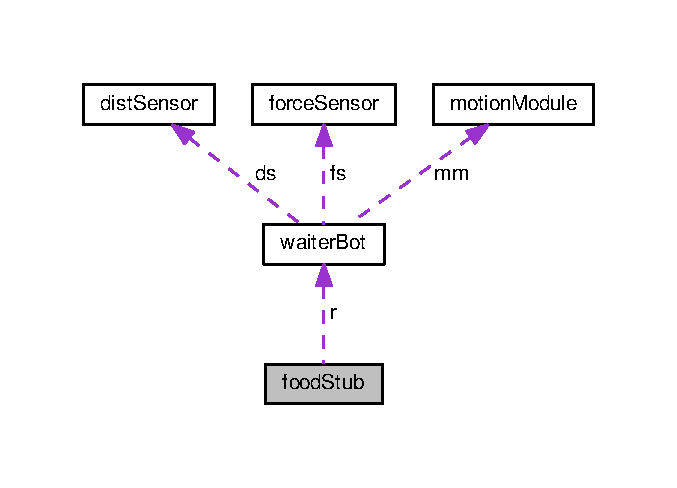
\includegraphics[width=325pt]{classfoodStub__coll__graph}
\end{center}
\end{figure}
\subsection*{Public Member Functions}
\begin{DoxyCompactItemize}
\item 
\hyperlink{classfoodStub_a8a60f219fd540ac7c68e46e2bcb98db2}{food\+Stub} ()
\begin{DoxyCompactList}\small\item\em Public Methods and Atrributes. \end{DoxyCompactList}\item 
float \hyperlink{classfoodStub_a5be8738657d5c4dccffc791024524b09}{get\+Food\+Weight} ()
\begin{DoxyCompactList}\small\item\em get food weight function \end{DoxyCompactList}\item 
void \hyperlink{classfoodStub_ae28a11ef20cf122cc9d547a25f34e1c9}{add\+Food} ()
\begin{DoxyCompactList}\small\item\em increase food weight function \end{DoxyCompactList}\item 
void \hyperlink{classfoodStub_ad60120dcd062bc14ba14f1a04bd798db}{remove\+Food} ()
\begin{DoxyCompactList}\small\item\em decrease food weight function \end{DoxyCompactList}\item 
std\+\_\+msgs\+::\+Float32 \hyperlink{classfoodStub_a4436ac50719f58831d6238ec2396764d}{pub\+Food} ()
\begin{DoxyCompactList}\small\item\em publish food weight function \end{DoxyCompactList}\end{DoxyCompactItemize}
\subsection*{Public Attributes}
\begin{DoxyCompactItemize}
\item 
\hyperlink{classwaiterBot}{waiter\+Bot} \hyperlink{classfoodStub_a88a32b2f907a471c65631dfffb24c787}{r}
\begin{DoxyCompactList}\small\item\em \hyperlink{classwaiterBot}{waiter\+Bot} \end{DoxyCompactList}\end{DoxyCompactItemize}


\subsection{Detailed Description}
A food stub Class. 

M\+IT License

Copyright 2017 Ruben Acevedo

Permission is hereby granted, free of charge, to any person obtaining a copy of this software and associated documentation files (the \char`\"{}\+Software\char`\"{}), to deal in the Software without restriction, including without limitation the rights to use, copy, modify, merge, publish, distribute, sublicense, and/or sell copies of the Software, and to permit persons to whom the Software is furnished to do so, subject to the following conditions\+:

The above copyright notice and this permission notice shall be included in all copies or substantial portions of the Software. T\+HE S\+O\+F\+T\+W\+A\+RE IS P\+R\+O\+V\+I\+D\+ED \char`\"{}\+A\+S I\+S\char`\"{}, W\+I\+T\+H\+O\+UT W\+A\+R\+R\+A\+N\+TY OF A\+NY K\+I\+ND, E\+X\+P\+R\+E\+SS OR I\+M\+P\+L\+I\+ED, I\+N\+C\+L\+U\+D\+I\+NG B\+UT N\+OT L\+I\+M\+I\+T\+ED TO T\+HE W\+A\+R\+R\+A\+N\+T\+I\+ES OF M\+E\+R\+C\+H\+A\+N\+T\+A\+B\+I\+L\+I\+TY, F\+I\+T\+N\+E\+SS F\+OR A P\+A\+R\+T\+I\+C\+U\+L\+AR P\+U\+R\+P\+O\+SE A\+ND N\+O\+N\+I\+N\+F\+R\+I\+N\+G\+E\+M\+E\+NT. IN NO E\+V\+E\+NT S\+H\+A\+LL T\+HE A\+U\+T\+H\+O\+RS OR C\+O\+P\+Y\+R\+I\+G\+HT H\+O\+L\+D\+E\+RS BE L\+I\+A\+B\+LE F\+OR A\+NY C\+L\+A\+IM, D\+A\+M\+A\+G\+ES OR O\+T\+H\+ER L\+I\+A\+B\+I\+L\+I\+TY, W\+H\+E\+T\+H\+ER IN AN A\+C\+T\+I\+ON OF C\+O\+N\+T\+R\+A\+CT, T\+O\+RT OR O\+T\+H\+E\+R\+W\+I\+SE, A\+R\+I\+S\+I\+NG F\+R\+OM, O\+UT OF OR IN C\+O\+N\+N\+E\+C\+T\+I\+ON W\+I\+TH T\+HE S\+O\+F\+T\+W\+A\+RE OR T\+HE U\+SE OR O\+T\+H\+ER D\+E\+A\+L\+I\+N\+GS IN T\+HE S\+O\+F\+T\+W\+A\+RE. © 2017 Git\+Hub, Inc. This class publishes food weight that the force sensor can read 

\subsection{Constructor \& Destructor Documentation}
\index{food\+Stub@{food\+Stub}!food\+Stub@{food\+Stub}}
\index{food\+Stub@{food\+Stub}!food\+Stub@{food\+Stub}}
\subsubsection[{\texorpdfstring{food\+Stub()}{foodStub()}}]{\setlength{\rightskip}{0pt plus 5cm}food\+Stub\+::food\+Stub (
\begin{DoxyParamCaption}
{}
\end{DoxyParamCaption}
)}\hypertarget{classfoodStub_a8a60f219fd540ac7c68e46e2bcb98db2}{}\label{classfoodStub_a8a60f219fd540ac7c68e46e2bcb98db2}


Public Methods and Atrributes. 

Class Constructor.

Class Constructor This code constructs the class. It initializes the food weight to be 0 Sets the removed\+Food\+When\+Stoped false 
\begin{DoxyParams}{Parameters}
{\em nothing} & \\
\hline
\end{DoxyParams}
\begin{DoxyReturn}{Returns}
nothing
\end{DoxyReturn}
M\+IT License

Copyright 2017 Ruben Acevedo

Permission is hereby granted, free of charge, to any person obtaining a copy of this software and associated documentation files (the \char`\"{}\+Software\char`\"{}), to deal in the Software without restriction, including without limitation the rights to use, copy, modify, merge, publish, distribute, sublicense, and/or sell copies of the Software, and to permit persons to whom the Software is furnished to do so, subject to the following conditions\+:

The above copyright notice and this permission notice shall be included in all copies or substantial portions of the Software. T\+HE S\+O\+F\+T\+W\+A\+RE IS P\+R\+O\+V\+I\+D\+ED \char`\"{}\+A\+S I\+S\char`\"{}, W\+I\+T\+H\+O\+UT W\+A\+R\+R\+A\+N\+TY OF A\+NY K\+I\+ND, E\+X\+P\+R\+E\+SS OR I\+M\+P\+L\+I\+ED, I\+N\+C\+L\+U\+D\+I\+NG B\+UT N\+OT L\+I\+M\+I\+T\+ED TO T\+HE W\+A\+R\+R\+A\+N\+T\+I\+ES OF M\+E\+R\+C\+H\+A\+N\+T\+A\+B\+I\+L\+I\+TY, F\+I\+T\+N\+E\+SS F\+OR A P\+A\+R\+T\+I\+C\+U\+L\+AR P\+U\+R\+P\+O\+SE A\+ND N\+O\+N\+I\+N\+F\+R\+I\+N\+G\+E\+M\+E\+NT. IN NO E\+V\+E\+NT S\+H\+A\+LL T\+HE A\+U\+T\+H\+O\+RS OR C\+O\+P\+Y\+R\+I\+G\+HT H\+O\+L\+D\+E\+RS BE L\+I\+A\+B\+LE F\+OR A\+NY C\+L\+A\+IM, D\+A\+M\+A\+G\+ES OR O\+T\+H\+ER L\+I\+A\+B\+I\+L\+I\+TY, W\+H\+E\+T\+H\+ER IN AN A\+C\+T\+I\+ON OF C\+O\+N\+T\+R\+A\+CT, T\+O\+RT OR O\+T\+H\+E\+R\+W\+I\+SE, A\+R\+I\+S\+I\+NG F\+R\+OM, O\+UT OF OR IN C\+O\+N\+N\+E\+C\+T\+I\+ON W\+I\+TH T\+HE S\+O\+F\+T\+W\+A\+RE OR T\+HE U\+SE OR O\+T\+H\+ER D\+E\+A\+L\+I\+N\+GS IN T\+HE S\+O\+F\+T\+W\+A\+RE. © 2017 Git\+Hub, Inc. This code constructs the class. It initializes the food weight to be 0 Sets the removed\+Food\+When\+Stoped false 
\begin{DoxyParams}{Parameters}
{\em nothing} & \\
\hline
\end{DoxyParams}
\begin{DoxyReturn}{Returns}
nothing 
\end{DoxyReturn}


\subsection{Member Function Documentation}
\index{food\+Stub@{food\+Stub}!add\+Food@{add\+Food}}
\index{add\+Food@{add\+Food}!food\+Stub@{food\+Stub}}
\subsubsection[{\texorpdfstring{add\+Food()}{addFood()}}]{\setlength{\rightskip}{0pt plus 5cm}void food\+Stub\+::add\+Food (
\begin{DoxyParamCaption}
{}
\end{DoxyParamCaption}
)}\hypertarget{classfoodStub_ae28a11ef20cf122cc9d547a25f34e1c9}{}\label{classfoodStub_ae28a11ef20cf122cc9d547a25f34e1c9}


increase food weight function 

This function increased the food weight to 25 N 
\begin{DoxyParams}{Parameters}
{\em nothing} & \\
\hline
\end{DoxyParams}
\begin{DoxyReturn}{Returns}
nothing
\end{DoxyReturn}
This function increased the food weight to 9 N 
\begin{DoxyParams}{Parameters}
{\em nothing} & \\
\hline
\end{DoxyParams}
\begin{DoxyReturn}{Returns}
nothing 
\end{DoxyReturn}
\index{food\+Stub@{food\+Stub}!get\+Food\+Weight@{get\+Food\+Weight}}
\index{get\+Food\+Weight@{get\+Food\+Weight}!food\+Stub@{food\+Stub}}
\subsubsection[{\texorpdfstring{get\+Food\+Weight()}{getFoodWeight()}}]{\setlength{\rightskip}{0pt plus 5cm}float food\+Stub\+::get\+Food\+Weight (
\begin{DoxyParamCaption}
{}
\end{DoxyParamCaption}
)}\hypertarget{classfoodStub_a5be8738657d5c4dccffc791024524b09}{}\label{classfoodStub_a5be8738657d5c4dccffc791024524b09}


get food weight function 

This code returns the food weight 
\begin{DoxyParams}{Parameters}
{\em nothing} & \\
\hline
\end{DoxyParams}
\begin{DoxyReturn}{Returns}
float repersenting the food\+Weight value 
\end{DoxyReturn}
\index{food\+Stub@{food\+Stub}!pub\+Food@{pub\+Food}}
\index{pub\+Food@{pub\+Food}!food\+Stub@{food\+Stub}}
\subsubsection[{\texorpdfstring{pub\+Food()}{pubFood()}}]{\setlength{\rightskip}{0pt plus 5cm}std\+\_\+msgs\+::\+Float32 food\+Stub\+::pub\+Food (
\begin{DoxyParamCaption}
{}
\end{DoxyParamCaption}
)}\hypertarget{classfoodStub_a4436ac50719f58831d6238ec2396764d}{}\label{classfoodStub_a4436ac50719f58831d6238ec2396764d}


publish food weight function 

This function returns the food publish message 
\begin{DoxyParams}{Parameters}
{\em nothing} & \\
\hline
\end{DoxyParams}
\begin{DoxyReturn}{Returns}
a std\+\_\+msgs\+::\+Float32 message repersenting the food weight 
\end{DoxyReturn}
\index{food\+Stub@{food\+Stub}!remove\+Food@{remove\+Food}}
\index{remove\+Food@{remove\+Food}!food\+Stub@{food\+Stub}}
\subsubsection[{\texorpdfstring{remove\+Food()}{removeFood()}}]{\setlength{\rightskip}{0pt plus 5cm}void food\+Stub\+::remove\+Food (
\begin{DoxyParamCaption}
{}
\end{DoxyParamCaption}
)}\hypertarget{classfoodStub_ad60120dcd062bc14ba14f1a04bd798db}{}\label{classfoodStub_ad60120dcd062bc14ba14f1a04bd798db}


decrease food weight function 

This function decreases the food weight by 5N 
\begin{DoxyParams}{Parameters}
{\em nothing} & \\
\hline
\end{DoxyParams}
\begin{DoxyReturn}{Returns}
nothing
\end{DoxyReturn}
This function decreases the food weight by 3 
\begin{DoxyParams}{Parameters}
{\em nothing} & \\
\hline
\end{DoxyParams}
\begin{DoxyReturn}{Returns}
nothing 
\end{DoxyReturn}


\subsection{Member Data Documentation}
\index{food\+Stub@{food\+Stub}!r@{r}}
\index{r@{r}!food\+Stub@{food\+Stub}}
\subsubsection[{\texorpdfstring{r}{r}}]{\setlength{\rightskip}{0pt plus 5cm}{\bf waiter\+Bot} food\+Stub\+::r}\hypertarget{classfoodStub_a88a32b2f907a471c65631dfffb24c787}{}\label{classfoodStub_a88a32b2f907a471c65631dfffb24c787}


\hyperlink{classwaiterBot}{waiter\+Bot} 

this \hyperlink{classwaiterBot}{waiter\+Bot} repersents the robot It is used to keep track of the robots position so the food stub know how much food it should output 

The documentation for this class was generated from the following files\+:\begin{DoxyCompactItemize}
\item 
/home/viki/catkin\+\_\+ws/src/\+Waiter\+Bot/waiter\+\_\+bot/include/\hyperlink{foodStub_8hpp}{food\+Stub.\+hpp}\item 
/home/viki/catkin\+\_\+ws/src/\+Waiter\+Bot/waiter\+\_\+bot/src/\hyperlink{foodStub_8cpp}{food\+Stub.\+cpp}\end{DoxyCompactItemize}

\hypertarget{classforceSensor}{}\section{force\+Sensor Class Reference}
\label{classforceSensor}\index{force\+Sensor@{force\+Sensor}}


A force sensor Class.  




{\ttfamily \#include $<$force\+Sensor.\+hpp$>$}

\subsection*{Public Member Functions}
\begin{DoxyCompactItemize}
\item 
\hyperlink{classforceSensor_a3551d62022f49183d58590f22a110908}{force\+Sensor} ()
\begin{DoxyCompactList}\small\item\em Public Methods. \end{DoxyCompactList}\item 
float \hyperlink{classforceSensor_abb1fb6c8888399dde382af45962fb8d6}{get\+Weight} ()
\begin{DoxyCompactList}\small\item\em get the weight function \end{DoxyCompactList}\item 
void \hyperlink{classforceSensor_a801613e7da1697c527f208a9f09f8c90}{set\+Weight\+Call\+Back} (const std\+\_\+msgs\+::\+Float32 \&force\+\_\+msg)
\begin{DoxyCompactList}\small\item\em set the weight function \end{DoxyCompactList}\end{DoxyCompactItemize}


\subsection{Detailed Description}
A force sensor Class. 

M\+IT License

Copyright 2017 Ruben Acevedo

Permission is hereby granted, free of charge, to any person obtaining a copy of this software and associated documentation files (the \char`\"{}\+Software\char`\"{}), to deal in the Software without restriction, including without limitation the rights to use, copy, modify, merge, publish, distribute, sublicense, and/or sell copies of the Software, and to permit persons to whom the Software is furnished to do so, subject to the following conditions\+:

The above copyright notice and this permission notice shall be included in all copies or substantial portions of the Software. T\+HE S\+O\+F\+T\+W\+A\+RE IS P\+R\+O\+V\+I\+D\+ED \char`\"{}\+A\+S I\+S\char`\"{}, W\+I\+T\+H\+O\+UT W\+A\+R\+R\+A\+N\+TY OF A\+NY K\+I\+ND, E\+X\+P\+R\+E\+SS OR I\+M\+P\+L\+I\+ED, I\+N\+C\+L\+U\+D\+I\+NG B\+UT N\+OT L\+I\+M\+I\+T\+ED TO T\+HE W\+A\+R\+R\+A\+N\+T\+I\+ES OF M\+E\+R\+C\+H\+A\+N\+T\+A\+B\+I\+L\+I\+TY, F\+I\+T\+N\+E\+SS F\+OR A P\+A\+R\+T\+I\+C\+U\+L\+AR P\+U\+R\+P\+O\+SE A\+ND N\+O\+N\+I\+N\+F\+R\+I\+N\+G\+E\+M\+E\+NT. IN NO E\+V\+E\+NT S\+H\+A\+LL T\+HE A\+U\+T\+H\+O\+RS OR C\+O\+P\+Y\+R\+I\+G\+HT H\+O\+L\+D\+E\+RS BE L\+I\+A\+B\+LE F\+OR A\+NY C\+L\+A\+IM, D\+A\+M\+A\+G\+ES OR O\+T\+H\+ER L\+I\+A\+B\+I\+L\+I\+TY, W\+H\+E\+T\+H\+ER IN AN A\+C\+T\+I\+ON OF C\+O\+N\+T\+R\+A\+CT, T\+O\+RT OR O\+T\+H\+E\+R\+W\+I\+SE, A\+R\+I\+S\+I\+NG F\+R\+OM, O\+UT OF OR IN C\+O\+N\+N\+E\+C\+T\+I\+ON W\+I\+TH T\+HE S\+O\+F\+T\+W\+A\+RE OR T\+HE U\+SE OR O\+T\+H\+ER D\+E\+A\+L\+I\+N\+GS IN T\+HE S\+O\+F\+T\+W\+A\+RE. © 2017 Git\+Hub, Inc. This class stores data from the force sensor 

\subsection{Constructor \& Destructor Documentation}
\index{force\+Sensor@{force\+Sensor}!force\+Sensor@{force\+Sensor}}
\index{force\+Sensor@{force\+Sensor}!force\+Sensor@{force\+Sensor}}
\subsubsection[{\texorpdfstring{force\+Sensor()}{forceSensor()}}]{\setlength{\rightskip}{0pt plus 5cm}force\+Sensor\+::force\+Sensor (
\begin{DoxyParamCaption}
{}
\end{DoxyParamCaption}
)}\hypertarget{classforceSensor_a3551d62022f49183d58590f22a110908}{}\label{classforceSensor_a3551d62022f49183d58590f22a110908}


Public Methods. 

Class Constructor.

Class Constructor This code constructs the class. It initializes the weight to be -\/1 
\begin{DoxyParams}{Parameters}
{\em nothing} & \\
\hline
\end{DoxyParams}
\begin{DoxyReturn}{Returns}
nothing
\end{DoxyReturn}
M\+IT License

Copyright 2017 Ruben Acevedo

Permission is hereby granted, free of charge, to any person obtaining a copy of this software and associated documentation files (the \char`\"{}\+Software\char`\"{}), to deal in the Software without restriction, including without limitation the rights to use, copy, modify, merge, publish, distribute, sublicense, and/or sell copies of the Software, and to permit persons to whom the Software is furnished to do so, subject to the following conditions\+:

The above copyright notice and this permission notice shall be included in all copies or substantial portions of the Software. T\+HE S\+O\+F\+T\+W\+A\+RE IS P\+R\+O\+V\+I\+D\+ED \char`\"{}\+A\+S I\+S\char`\"{}, W\+I\+T\+H\+O\+UT W\+A\+R\+R\+A\+N\+TY OF A\+NY K\+I\+ND, E\+X\+P\+R\+E\+SS OR I\+M\+P\+L\+I\+ED, I\+N\+C\+L\+U\+D\+I\+NG B\+UT N\+OT L\+I\+M\+I\+T\+ED TO T\+HE W\+A\+R\+R\+A\+N\+T\+I\+ES OF M\+E\+R\+C\+H\+A\+N\+T\+A\+B\+I\+L\+I\+TY, F\+I\+T\+N\+E\+SS F\+OR A P\+A\+R\+T\+I\+C\+U\+L\+AR P\+U\+R\+P\+O\+SE A\+ND N\+O\+N\+I\+N\+F\+R\+I\+N\+G\+E\+M\+E\+NT. IN NO E\+V\+E\+NT S\+H\+A\+LL T\+HE A\+U\+T\+H\+O\+RS OR C\+O\+P\+Y\+R\+I\+G\+HT H\+O\+L\+D\+E\+RS BE L\+I\+A\+B\+LE F\+OR A\+NY C\+L\+A\+IM, D\+A\+M\+A\+G\+ES OR O\+T\+H\+ER L\+I\+A\+B\+I\+L\+I\+TY, W\+H\+E\+T\+H\+ER IN AN A\+C\+T\+I\+ON OF C\+O\+N\+T\+R\+A\+CT, T\+O\+RT OR O\+T\+H\+E\+R\+W\+I\+SE, A\+R\+I\+S\+I\+NG F\+R\+OM, O\+UT OF OR IN C\+O\+N\+N\+E\+C\+T\+I\+ON W\+I\+TH T\+HE S\+O\+F\+T\+W\+A\+RE OR T\+HE U\+SE OR O\+T\+H\+ER D\+E\+A\+L\+I\+N\+GS IN T\+HE S\+O\+F\+T\+W\+A\+RE. © 2017 Git\+Hub, Inc. This code constructs the class. It initializes the weight to be -\/1 
\begin{DoxyParams}{Parameters}
{\em nothing} & \\
\hline
\end{DoxyParams}
\begin{DoxyReturn}{Returns}
nothing 
\end{DoxyReturn}


\subsection{Member Function Documentation}
\index{force\+Sensor@{force\+Sensor}!get\+Weight@{get\+Weight}}
\index{get\+Weight@{get\+Weight}!force\+Sensor@{force\+Sensor}}
\subsubsection[{\texorpdfstring{get\+Weight()}{getWeight()}}]{\setlength{\rightskip}{0pt plus 5cm}float force\+Sensor\+::get\+Weight (
\begin{DoxyParamCaption}
{}
\end{DoxyParamCaption}
)}\hypertarget{classforceSensor_abb1fb6c8888399dde382af45962fb8d6}{}\label{classforceSensor_abb1fb6c8888399dde382af45962fb8d6}


get the weight function 

This function gets the weight value 
\begin{DoxyParams}{Parameters}
{\em nothing} & \\
\hline
\end{DoxyParams}
\begin{DoxyReturn}{Returns}
float repesenting the weight value 
\end{DoxyReturn}
\index{force\+Sensor@{force\+Sensor}!set\+Weight\+Call\+Back@{set\+Weight\+Call\+Back}}
\index{set\+Weight\+Call\+Back@{set\+Weight\+Call\+Back}!force\+Sensor@{force\+Sensor}}
\subsubsection[{\texorpdfstring{set\+Weight\+Call\+Back(const std\+\_\+msgs\+::\+Float32 \&force\+\_\+msg)}{setWeightCallBack(const std_msgs::Float32 &force_msg)}}]{\setlength{\rightskip}{0pt plus 5cm}void force\+Sensor\+::set\+Weight\+Call\+Back (
\begin{DoxyParamCaption}
\item[{const std\+\_\+msgs\+::\+Float32 \&}]{force\+\_\+msg}
\end{DoxyParamCaption}
)}\hypertarget{classforceSensor_a801613e7da1697c527f208a9f09f8c90}{}\label{classforceSensor_a801613e7da1697c527f208a9f09f8c90}


set the weight function 

This function sets the weight value 
\begin{DoxyParams}{Parameters}
{\em a} & const std\+\_\+msgs\+::\+Float32 reference message type repersenting the values that the force sensor reads \\
\hline
\end{DoxyParams}
\begin{DoxyReturn}{Returns}
nothing 
\end{DoxyReturn}


The documentation for this class was generated from the following files\+:\begin{DoxyCompactItemize}
\item 
/home/viki/catkin\+\_\+ws/src/\+Waiter\+Bot/waiter\+\_\+bot/include/\hyperlink{forceSensor_8hpp}{force\+Sensor.\+hpp}\item 
/home/viki/catkin\+\_\+ws/src/\+Waiter\+Bot/waiter\+\_\+bot/src/\hyperlink{forceSensor_8cpp}{force\+Sensor.\+cpp}\end{DoxyCompactItemize}

\hypertarget{classmotionModule}{}\section{motion\+Module Class Reference}
\label{classmotionModule}\index{motion\+Module@{motion\+Module}}


A motion module Class.  




{\ttfamily \#include $<$motion\+Module.\+hpp$>$}

\subsection*{Public Member Functions}
\begin{DoxyCompactItemize}
\item 
\hyperlink{classmotionModule_a61a9ef6897e181d2ba0a34494948e2b2}{motion\+Module} ()
\begin{DoxyCompactList}\small\item\em Public Methods. \end{DoxyCompactList}\item 
bool \hyperlink{classmotionModule_a57bffc2f83a9a05f69ab698875d6b0a8}{in\+Region} (\hyperlink{classposition}{position} pos)
\begin{DoxyCompactList}\small\item\em checks to see if the robot is in a region \end{DoxyCompactList}\item 
\hyperlink{classposition}{position} \hyperlink{classmotionModule_a8ee6c6f8a047df26cd82166a5342bac4}{get\+Current\+Loc} ()
\begin{DoxyCompactList}\small\item\em gets the robots current location \end{DoxyCompactList}\item 
void \hyperlink{classmotionModule_afd1bb61853930200af6989569ac6a860}{set\+Current\+Location\+Call\+Back} (const nav\+\_\+msgs\+::\+Odometry \&odo\+\_\+msg)
\begin{DoxyCompactList}\small\item\em sets the current location of the robot \end{DoxyCompactList}\item 
void \hyperlink{classmotionModule_afe21651bb696b248e121817573fabbbd}{set\+Theta\+Value\+For\+Tests} (const float \&t)
\begin{DoxyCompactList}\small\item\em sets the current location\textquotesingle{}s theta of the robot \end{DoxyCompactList}\end{DoxyCompactItemize}


\subsection{Detailed Description}
A motion module Class. 

M\+IT License

Copyright 2017 Ruben Acevedo

Permission is hereby granted, free of charge, to any person obtaining a copy of this software and associated documentation files (the \char`\"{}\+Software\char`\"{}), to deal in the Software without restriction, including without limitation the rights to use, copy, modify, merge, publish, distribute, sublicense, and/or sell copies of the Software, and to permit persons to whom the Software is furnished to do so, subject to the following conditions\+:

The above copyright notice and this permission notice shall be included in all copies or substantial portions of the Software. T\+HE S\+O\+F\+T\+W\+A\+RE IS P\+R\+O\+V\+I\+D\+ED \char`\"{}\+A\+S I\+S\char`\"{}, W\+I\+T\+H\+O\+UT W\+A\+R\+R\+A\+N\+TY OF A\+NY K\+I\+ND, E\+X\+P\+R\+E\+SS OR I\+M\+P\+L\+I\+ED, I\+N\+C\+L\+U\+D\+I\+NG B\+UT N\+OT L\+I\+M\+I\+T\+ED TO T\+HE W\+A\+R\+R\+A\+N\+T\+I\+ES OF M\+E\+R\+C\+H\+A\+N\+T\+A\+B\+I\+L\+I\+TY, F\+I\+T\+N\+E\+SS F\+OR A P\+A\+R\+T\+I\+C\+U\+L\+AR P\+U\+R\+P\+O\+SE A\+ND N\+O\+N\+I\+N\+F\+R\+I\+N\+G\+E\+M\+E\+NT. IN NO E\+V\+E\+NT S\+H\+A\+LL T\+HE A\+U\+T\+H\+O\+RS OR C\+O\+P\+Y\+R\+I\+G\+HT H\+O\+L\+D\+E\+RS BE L\+I\+A\+B\+LE F\+OR A\+NY C\+L\+A\+IM, D\+A\+M\+A\+G\+ES OR O\+T\+H\+ER L\+I\+A\+B\+I\+L\+I\+TY, W\+H\+E\+T\+H\+ER IN AN A\+C\+T\+I\+ON OF C\+O\+N\+T\+R\+A\+CT, T\+O\+RT OR O\+T\+H\+E\+R\+W\+I\+SE, A\+R\+I\+S\+I\+NG F\+R\+OM, O\+UT OF OR IN C\+O\+N\+N\+E\+C\+T\+I\+ON W\+I\+TH T\+HE S\+O\+F\+T\+W\+A\+RE OR T\+HE U\+SE OR O\+T\+H\+ER D\+E\+A\+L\+I\+N\+GS IN T\+HE S\+O\+F\+T\+W\+A\+RE. © 2017 Git\+Hub, Inc. This class keeps track of the robot\textquotesingle{}s motion in the map 

\subsection{Constructor \& Destructor Documentation}
\index{motion\+Module@{motion\+Module}!motion\+Module@{motion\+Module}}
\index{motion\+Module@{motion\+Module}!motion\+Module@{motion\+Module}}
\subsubsection[{\texorpdfstring{motion\+Module()}{motionModule()}}]{\setlength{\rightskip}{0pt plus 5cm}motion\+Module\+::motion\+Module (
\begin{DoxyParamCaption}
{}
\end{DoxyParamCaption}
)}\hypertarget{classmotionModule_a61a9ef6897e181d2ba0a34494948e2b2}{}\label{classmotionModule_a61a9ef6897e181d2ba0a34494948e2b2}


Public Methods. 

Class Constructor.

Class Constructor This code constructs the class. 
\begin{DoxyParams}{Parameters}
{\em nothing} & \\
\hline
\end{DoxyParams}
\begin{DoxyReturn}{Returns}
nothing
\end{DoxyReturn}
M\+IT License

Copyright 2017 Ruben Acevedo

Permission is hereby granted, free of charge, to any person obtaining a copy of this software and associated documentation files (the \char`\"{}\+Software\char`\"{}), to deal in the Software without restriction, including without limitation the rights to use, copy, modify, merge, publish, distribute, sublicense, and/or sell copies of the Software, and to permit persons to whom the Software is furnished to do so, subject to the following conditions\+:

The above copyright notice and this permission notice shall be included in all copies or substantial portions of the Software. T\+HE S\+O\+F\+T\+W\+A\+RE IS P\+R\+O\+V\+I\+D\+ED \char`\"{}\+A\+S I\+S\char`\"{}, W\+I\+T\+H\+O\+UT W\+A\+R\+R\+A\+N\+TY OF A\+NY K\+I\+ND, E\+X\+P\+R\+E\+SS OR I\+M\+P\+L\+I\+ED, I\+N\+C\+L\+U\+D\+I\+NG B\+UT N\+OT L\+I\+M\+I\+T\+ED TO T\+HE W\+A\+R\+R\+A\+N\+T\+I\+ES OF M\+E\+R\+C\+H\+A\+N\+T\+A\+B\+I\+L\+I\+TY, F\+I\+T\+N\+E\+SS F\+OR A P\+A\+R\+T\+I\+C\+U\+L\+AR P\+U\+R\+P\+O\+SE A\+ND N\+O\+N\+I\+N\+F\+R\+I\+N\+G\+E\+M\+E\+NT. IN NO E\+V\+E\+NT S\+H\+A\+LL T\+HE A\+U\+T\+H\+O\+RS OR C\+O\+P\+Y\+R\+I\+G\+HT H\+O\+L\+D\+E\+RS BE L\+I\+A\+B\+LE F\+OR A\+NY C\+L\+A\+IM, D\+A\+M\+A\+G\+ES OR O\+T\+H\+ER L\+I\+A\+B\+I\+L\+I\+TY, W\+H\+E\+T\+H\+ER IN AN A\+C\+T\+I\+ON OF C\+O\+N\+T\+R\+A\+CT, T\+O\+RT OR O\+T\+H\+E\+R\+W\+I\+SE, A\+R\+I\+S\+I\+NG F\+R\+OM, O\+UT OF OR IN C\+O\+N\+N\+E\+C\+T\+I\+ON W\+I\+TH T\+HE S\+O\+F\+T\+W\+A\+RE OR T\+HE U\+SE OR O\+T\+H\+ER D\+E\+A\+L\+I\+N\+GS IN T\+HE S\+O\+F\+T\+W\+A\+RE. © 2017 Git\+Hub, Inc. This code constructs the class. 
\begin{DoxyParams}{Parameters}
{\em nothing} & \\
\hline
\end{DoxyParams}
\begin{DoxyReturn}{Returns}
nothing 
\end{DoxyReturn}


\subsection{Member Function Documentation}
\index{motion\+Module@{motion\+Module}!get\+Current\+Loc@{get\+Current\+Loc}}
\index{get\+Current\+Loc@{get\+Current\+Loc}!motion\+Module@{motion\+Module}}
\subsubsection[{\texorpdfstring{get\+Current\+Loc()}{getCurrentLoc()}}]{\setlength{\rightskip}{0pt plus 5cm}{\bf position} motion\+Module\+::get\+Current\+Loc (
\begin{DoxyParamCaption}
{}
\end{DoxyParamCaption}
)}\hypertarget{classmotionModule_a8ee6c6f8a047df26cd82166a5342bac4}{}\label{classmotionModule_a8ee6c6f8a047df26cd82166a5342bac4}


gets the robots current location 

This function returns the robots current\+Loc position 
\begin{DoxyParams}{Parameters}
{\em nothing} & \\
\hline
\end{DoxyParams}
\begin{DoxyReturn}{Returns}
a position repesenting the current\+Loc value 
\end{DoxyReturn}
\index{motion\+Module@{motion\+Module}!in\+Region@{in\+Region}}
\index{in\+Region@{in\+Region}!motion\+Module@{motion\+Module}}
\subsubsection[{\texorpdfstring{in\+Region(position pos)}{inRegion(position pos)}}]{\setlength{\rightskip}{0pt plus 5cm}bool motion\+Module\+::in\+Region (
\begin{DoxyParamCaption}
\item[{{\bf position}}]{pos}
\end{DoxyParamCaption}
)}\hypertarget{classmotionModule_a57bffc2f83a9a05f69ab698875d6b0a8}{}\label{classmotionModule_a57bffc2f83a9a05f69ab698875d6b0a8}


checks to see if the robot is in a region 

This function checks if the robot is in a region The robot should be with in 0.\+2 m of the pos for it to return that it is within the region 
\begin{DoxyParams}{Parameters}
{\em a} & position reference repersenting the target region \\
\hline
\end{DoxyParams}
\begin{DoxyReturn}{Returns}
bool repesenting whether the robot is in the region or not 
\end{DoxyReturn}
\index{motion\+Module@{motion\+Module}!set\+Current\+Location\+Call\+Back@{set\+Current\+Location\+Call\+Back}}
\index{set\+Current\+Location\+Call\+Back@{set\+Current\+Location\+Call\+Back}!motion\+Module@{motion\+Module}}
\subsubsection[{\texorpdfstring{set\+Current\+Location\+Call\+Back(const nav\+\_\+msgs\+::\+Odometry \&odo\+\_\+msg)}{setCurrentLocationCallBack(const nav_msgs::Odometry &odo_msg)}}]{\setlength{\rightskip}{0pt plus 5cm}void motion\+Module\+::set\+Current\+Location\+Call\+Back (
\begin{DoxyParamCaption}
\item[{const nav\+\_\+msgs\+::\+Odometry \&}]{odo\+\_\+msg}
\end{DoxyParamCaption}
)}\hypertarget{classmotionModule_afd1bb61853930200af6989569ac6a860}{}\label{classmotionModule_afd1bb61853930200af6989569ac6a860}


sets the current location of the robot 

This function sets the current location of the robot. it takes the nav\+\_\+msgs\+::\+Odometry message and converts it to a position. It sets that postion to be current\+Loc 
\begin{DoxyParams}{Parameters}
{\em a} & const nav\+\_\+msgs\+::\+Odometry message reference from the odometry sensor \\
\hline
\end{DoxyParams}
\begin{DoxyReturn}{Returns}
nothing 
\end{DoxyReturn}
\index{motion\+Module@{motion\+Module}!set\+Theta\+Value\+For\+Tests@{set\+Theta\+Value\+For\+Tests}}
\index{set\+Theta\+Value\+For\+Tests@{set\+Theta\+Value\+For\+Tests}!motion\+Module@{motion\+Module}}
\subsubsection[{\texorpdfstring{set\+Theta\+Value\+For\+Tests(const float \&t)}{setThetaValueForTests(const float &t)}}]{\setlength{\rightskip}{0pt plus 5cm}void motion\+Module\+::set\+Theta\+Value\+For\+Tests (
\begin{DoxyParamCaption}
\item[{const float \&}]{t}
\end{DoxyParamCaption}
)}\hypertarget{classmotionModule_afe21651bb696b248e121817573fabbbd}{}\label{classmotionModule_afe21651bb696b248e121817573fabbbd}


sets the current location\textquotesingle{}s theta of the robot 

This function sets the current location theta of the robot. this function is purely to make testing easier 
\begin{DoxyParams}{Parameters}
{\em a} & const float repesenting the theta \\
\hline
\end{DoxyParams}
\begin{DoxyReturn}{Returns}
nothing 
\end{DoxyReturn}


The documentation for this class was generated from the following files\+:\begin{DoxyCompactItemize}
\item 
/home/viki/catkin\+\_\+ws/src/\+Waiter\+Bot/waiter\+\_\+bot/include/\hyperlink{motionModule_8hpp}{motion\+Module.\+hpp}\item 
/home/viki/catkin\+\_\+ws/src/\+Waiter\+Bot/waiter\+\_\+bot/src/\hyperlink{motionModule_8cpp}{motion\+Module.\+cpp}\end{DoxyCompactItemize}

\hypertarget{classposition}{}\section{position Class Reference}
\label{classposition}\index{position@{position}}


A Position Class.  




{\ttfamily \#include $<$position.\+hpp$>$}

\subsection*{Public Member Functions}
\begin{DoxyCompactItemize}
\item 
\hyperlink{classposition_a0492eb9ae0eee02f191f02e229af24d1}{position} ()
\begin{DoxyCompactList}\small\item\em Public Methods. \end{DoxyCompactList}\item 
void \hyperlink{classposition_a64903875492810b4c4a8f0577406e620}{set\+Position} (const float \&\hyperlink{nodeInteractionsTest_8cpp_ad0da36b2558901e21e7a30f6c227a45e}{x}, const float \&y, const float \&t)
\begin{DoxyCompactList}\small\item\em Set the Position Function. \end{DoxyCompactList}\item 
std\+::vector$<$ float $>$ \hyperlink{classposition_a8c7fc88bef973ae597d039e14908c9c3}{get\+Pos} ()
\begin{DoxyCompactList}\small\item\em get the position function \end{DoxyCompactList}\end{DoxyCompactItemize}


\subsection{Detailed Description}
A Position Class. 

M\+IT License

Copyright 2017 Ruben Acevedo

Permission is hereby granted, free of charge, to any person obtaining a copy of this software and associated documentation files (the \char`\"{}\+Software\char`\"{}), to deal in the Software without restriction, including without limitation the rights to use, copy, modify, merge, publish, distribute, sublicense, and/or sell copies of the Software, and to permit persons to whom the Software is furnished to do so, subject to the following conditions\+:

The above copyright notice and this permission notice shall be included in all copies or substantial portions of the Software. T\+HE S\+O\+F\+T\+W\+A\+RE IS P\+R\+O\+V\+I\+D\+ED \char`\"{}\+A\+S I\+S\char`\"{}, W\+I\+T\+H\+O\+UT W\+A\+R\+R\+A\+N\+TY OF A\+NY K\+I\+ND, E\+X\+P\+R\+E\+SS OR I\+M\+P\+L\+I\+ED, I\+N\+C\+L\+U\+D\+I\+NG B\+UT N\+OT L\+I\+M\+I\+T\+ED TO T\+HE W\+A\+R\+R\+A\+N\+T\+I\+ES OF M\+E\+R\+C\+H\+A\+N\+T\+A\+B\+I\+L\+I\+TY, F\+I\+T\+N\+E\+SS F\+OR A P\+A\+R\+T\+I\+C\+U\+L\+AR P\+U\+R\+P\+O\+SE A\+ND N\+O\+N\+I\+N\+F\+R\+I\+N\+G\+E\+M\+E\+NT. IN NO E\+V\+E\+NT S\+H\+A\+LL T\+HE A\+U\+T\+H\+O\+RS OR C\+O\+P\+Y\+R\+I\+G\+HT H\+O\+L\+D\+E\+RS BE L\+I\+A\+B\+LE F\+OR A\+NY C\+L\+A\+IM, D\+A\+M\+A\+G\+ES OR O\+T\+H\+ER L\+I\+A\+B\+I\+L\+I\+TY, W\+H\+E\+T\+H\+ER IN AN A\+C\+T\+I\+ON OF C\+O\+N\+T\+R\+A\+CT, T\+O\+RT OR O\+T\+H\+E\+R\+W\+I\+SE, A\+R\+I\+S\+I\+NG F\+R\+OM, O\+UT OF OR IN C\+O\+N\+N\+E\+C\+T\+I\+ON W\+I\+TH T\+HE S\+O\+F\+T\+W\+A\+RE OR T\+HE U\+SE OR O\+T\+H\+ER D\+E\+A\+L\+I\+N\+GS IN T\+HE S\+O\+F\+T\+W\+A\+RE. © 2017 Git\+Hub, Inc. This class defines a position 

\subsection{Constructor \& Destructor Documentation}
\index{position@{position}!position@{position}}
\index{position@{position}!position@{position}}
\subsubsection[{\texorpdfstring{position()}{position()}}]{\setlength{\rightskip}{0pt plus 5cm}position\+::position (
\begin{DoxyParamCaption}
{}
\end{DoxyParamCaption}
)}\hypertarget{classposition_a0492eb9ae0eee02f191f02e229af24d1}{}\label{classposition_a0492eb9ae0eee02f191f02e229af24d1}


Public Methods. 

Class Constructor.

Class Constructor This code constructs the class. It initializes the xpos=ypos=theta=0 
\begin{DoxyParams}{Parameters}
{\em nothing} & \\
\hline
\end{DoxyParams}
\begin{DoxyReturn}{Returns}
nothing
\end{DoxyReturn}
M\+IT License

Copyright 2017 Ruben Acevedo

Permission is hereby granted, free of charge, to any person obtaining a copy of this software and associated documentation files (the \char`\"{}\+Software\char`\"{}), to deal in the Software without restriction, including without limitation the rights to use, copy, modify, merge, publish, distribute, sublicense, and/or sell copies of the Software, and to permit persons to whom the Software is furnished to do so, subject to the following conditions\+:

The above copyright notice and this permission notice shall be included in all copies or substantial portions of the Software. T\+HE S\+O\+F\+T\+W\+A\+RE IS P\+R\+O\+V\+I\+D\+ED \char`\"{}\+A\+S I\+S\char`\"{}, W\+I\+T\+H\+O\+UT W\+A\+R\+R\+A\+N\+TY OF A\+NY K\+I\+ND, E\+X\+P\+R\+E\+SS OR I\+M\+P\+L\+I\+ED, I\+N\+C\+L\+U\+D\+I\+NG B\+UT N\+OT L\+I\+M\+I\+T\+ED TO T\+HE W\+A\+R\+R\+A\+N\+T\+I\+ES OF M\+E\+R\+C\+H\+A\+N\+T\+A\+B\+I\+L\+I\+TY, F\+I\+T\+N\+E\+SS F\+OR A P\+A\+R\+T\+I\+C\+U\+L\+AR P\+U\+R\+P\+O\+SE A\+ND N\+O\+N\+I\+N\+F\+R\+I\+N\+G\+E\+M\+E\+NT. IN NO E\+V\+E\+NT S\+H\+A\+LL T\+HE A\+U\+T\+H\+O\+RS OR C\+O\+P\+Y\+R\+I\+G\+HT H\+O\+L\+D\+E\+RS BE L\+I\+A\+B\+LE F\+OR A\+NY C\+L\+A\+IM, D\+A\+M\+A\+G\+ES OR O\+T\+H\+ER L\+I\+A\+B\+I\+L\+I\+TY, W\+H\+E\+T\+H\+ER IN AN A\+C\+T\+I\+ON OF C\+O\+N\+T\+R\+A\+CT, T\+O\+RT OR O\+T\+H\+E\+R\+W\+I\+SE, A\+R\+I\+S\+I\+NG F\+R\+OM, O\+UT OF OR IN C\+O\+N\+N\+E\+C\+T\+I\+ON W\+I\+TH T\+HE S\+O\+F\+T\+W\+A\+RE OR T\+HE U\+SE OR O\+T\+H\+ER D\+E\+A\+L\+I\+N\+GS IN T\+HE S\+O\+F\+T\+W\+A\+RE. © 2017 Git\+Hub, Inc. This code constructs the class. It initializes the xpos=ypos=theta=0 
\begin{DoxyParams}{Parameters}
{\em nothing} & \\
\hline
\end{DoxyParams}
\begin{DoxyReturn}{Returns}
nothing 
\end{DoxyReturn}


\subsection{Member Function Documentation}
\index{position@{position}!get\+Pos@{get\+Pos}}
\index{get\+Pos@{get\+Pos}!position@{position}}
\subsubsection[{\texorpdfstring{get\+Pos()}{getPos()}}]{\setlength{\rightskip}{0pt plus 5cm}std\+::vector$<$ float $>$ position\+::get\+Pos (
\begin{DoxyParamCaption}
{}
\end{DoxyParamCaption}
)}\hypertarget{classposition_a8c7fc88bef973ae597d039e14908c9c3}{}\label{classposition_a8c7fc88bef973ae597d039e14908c9c3}


get the position function 

This function returns the stored position in the form of a vector where the first element is xpos, the second is y pos, and the third is theta 
\begin{DoxyParams}{Parameters}
{\em nothing} & \\
\hline
\end{DoxyParams}
\begin{DoxyReturn}{Returns}
a float vector repesenting the position 
\end{DoxyReturn}
\index{position@{position}!set\+Position@{set\+Position}}
\index{set\+Position@{set\+Position}!position@{position}}
\subsubsection[{\texorpdfstring{set\+Position(const float \&x, const float \&y, const float \&t)}{setPosition(const float &x, const float &y, const float &t)}}]{\setlength{\rightskip}{0pt plus 5cm}void position\+::set\+Position (
\begin{DoxyParamCaption}
\item[{const float \&}]{x, }
\item[{const float \&}]{y, }
\item[{const float \&}]{t}
\end{DoxyParamCaption}
)}\hypertarget{classposition_a64903875492810b4c4a8f0577406e620}{}\label{classposition_a64903875492810b4c4a8f0577406e620}


Set the Position Function. 

This sets the postion 
\begin{DoxyParams}{Parameters}
{\em a} & const float reference for the x coordinate \\
\hline
{\em a} & const float reference for the y coordinate \\
\hline
{\em a} & const float reference for the theta coordinate \\
\hline
\end{DoxyParams}
\begin{DoxyReturn}{Returns}
nothing 
\end{DoxyReturn}


The documentation for this class was generated from the following files\+:\begin{DoxyCompactItemize}
\item 
/home/viki/catkin\+\_\+ws/src/\+Waiter\+Bot/waiter\+\_\+bot/include/\hyperlink{position_8hpp}{position.\+hpp}\item 
/home/viki/catkin\+\_\+ws/src/\+Waiter\+Bot/waiter\+\_\+bot/src/\hyperlink{position_8cpp}{position.\+cpp}\end{DoxyCompactItemize}

\hypertarget{classwaiterBot}{}\section{waiter\+Bot Class Reference}
\label{classwaiterBot}\index{waiter\+Bot@{waiter\+Bot}}


A \hyperlink{classwaiterBot}{waiter\+Bot} Class.  




{\ttfamily \#include $<$waiter\+Bot.\+hpp$>$}



Collaboration diagram for waiter\+Bot\+:
\nopagebreak
\begin{figure}[H]
\begin{center}
\leavevmode
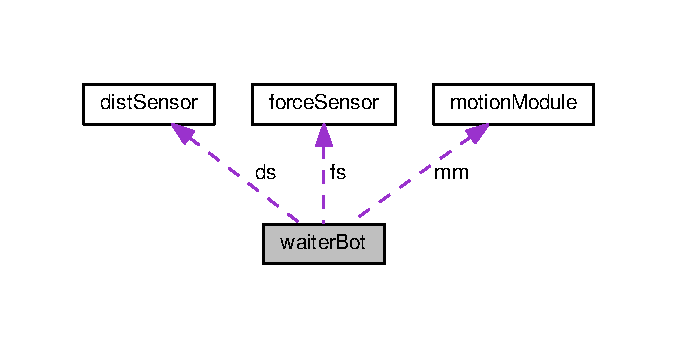
\includegraphics[width=325pt]{classwaiterBot__coll__graph}
\end{center}
\end{figure}
\subsection*{Public Member Functions}
\begin{DoxyCompactItemize}
\item 
\hyperlink{classwaiterBot_a9b3a45ca6b7700aa82ae8496aa85f2b3}{waiter\+Bot} ()
\begin{DoxyCompactList}\small\item\em Public Methods and Attributes. \end{DoxyCompactList}\item 
std\+::string \hyperlink{classwaiterBot_a877f608ceff919a2c18082de76bb39f7}{get\+Status} ()
\begin{DoxyCompactList}\small\item\em return the robot\textquotesingle{}s status function \end{DoxyCompactList}\item 
std\+::vector$<$ \hyperlink{classposition}{position} $>$ \hyperlink{classwaiterBot_a9ee50a152a69fcf37133892d149ec352}{get\+Target\+Locs} ()
\begin{DoxyCompactList}\small\item\em gets the robot\textquotesingle{}s target locations \end{DoxyCompactList}\item 
bool \hyperlink{classwaiterBot_a20494335cbe4d278c04c7e7d0440b037}{did\+Stop} ()
\begin{DoxyCompactList}\small\item\em sees if the robot stopped function \end{DoxyCompactList}\item 
float \hyperlink{classwaiterBot_a7269cbb34bbca97f1002206079fdbfe1}{get\+Angle\+Diff} (\hyperlink{classposition}{position} tl)
\begin{DoxyCompactList}\small\item\em get the angle difference function \end{DoxyCompactList}\item 
geometry\+\_\+msgs\+::\+Twist \hyperlink{classwaiterBot_a1c6e589b55155bae665dde42d664a292}{move} ()
\begin{DoxyCompactList}\small\item\em sees if the robot stopped function \end{DoxyCompactList}\end{DoxyCompactItemize}
\subsection*{Public Attributes}
\begin{DoxyCompactItemize}
\item 
\hyperlink{classdistSensor}{dist\+Sensor} \hyperlink{classwaiterBot_a54139b99410779ba1a3af03d45dd3dec}{ds}
\begin{DoxyCompactList}\small\item\em the \hyperlink{classwaiterBot}{waiter\+Bot}\textquotesingle{}s distance Sensor \end{DoxyCompactList}\item 
\hyperlink{classmotionModule}{motion\+Module} \hyperlink{classwaiterBot_aa477504a694726fc90b8e6fa4bcc9998}{mm}
\begin{DoxyCompactList}\small\item\em the \hyperlink{classwaiterBot}{waiter\+Bot}\textquotesingle{}s motion module \end{DoxyCompactList}\item 
\hyperlink{classforceSensor}{force\+Sensor} \hyperlink{classwaiterBot_a359f1ca46275a20771b0f922268fb72e}{fs}
\begin{DoxyCompactList}\small\item\em the \hyperlink{classwaiterBot}{waiter\+Bot}\textquotesingle{}s force sensor \end{DoxyCompactList}\end{DoxyCompactItemize}


\subsection{Detailed Description}
A \hyperlink{classwaiterBot}{waiter\+Bot} Class. 

M\+IT License

Copyright 2017 Ruben Acevedo

Permission is hereby granted, free of charge, to any person obtaining a copy of this software and associated documentation files (the \char`\"{}\+Software\char`\"{}), to deal in the Software without restriction, including without limitation the rights to use, copy, modify, merge, publish, distribute, sublicense, and/or sell copies of the Software, and to permit persons to whom the Software is furnished to do so, subject to the following conditions\+:

The above copyright notice and this permission notice shall be included in all copies or substantial portions of the Software. T\+HE S\+O\+F\+T\+W\+A\+RE IS P\+R\+O\+V\+I\+D\+ED \char`\"{}\+A\+S I\+S\char`\"{}, W\+I\+T\+H\+O\+UT W\+A\+R\+R\+A\+N\+TY OF A\+NY K\+I\+ND, E\+X\+P\+R\+E\+SS OR I\+M\+P\+L\+I\+ED, I\+N\+C\+L\+U\+D\+I\+NG B\+UT N\+OT L\+I\+M\+I\+T\+ED TO T\+HE W\+A\+R\+R\+A\+N\+T\+I\+ES OF M\+E\+R\+C\+H\+A\+N\+T\+A\+B\+I\+L\+I\+TY, F\+I\+T\+N\+E\+SS F\+OR A P\+A\+R\+T\+I\+C\+U\+L\+AR P\+U\+R\+P\+O\+SE A\+ND N\+O\+N\+I\+N\+F\+R\+I\+N\+G\+E\+M\+E\+NT. IN NO E\+V\+E\+NT S\+H\+A\+LL T\+HE A\+U\+T\+H\+O\+RS OR C\+O\+P\+Y\+R\+I\+G\+HT H\+O\+L\+D\+E\+RS BE L\+I\+A\+B\+LE F\+OR A\+NY C\+L\+A\+IM, D\+A\+M\+A\+G\+ES OR O\+T\+H\+ER L\+I\+A\+B\+I\+L\+I\+TY, W\+H\+E\+T\+H\+ER IN AN A\+C\+T\+I\+ON OF C\+O\+N\+T\+R\+A\+CT, T\+O\+RT OR O\+T\+H\+E\+R\+W\+I\+SE, A\+R\+I\+S\+I\+NG F\+R\+OM, O\+UT OF OR IN C\+O\+N\+N\+E\+C\+T\+I\+ON W\+I\+TH T\+HE S\+O\+F\+T\+W\+A\+RE OR T\+HE U\+SE OR O\+T\+H\+ER D\+E\+A\+L\+I\+N\+GS IN T\+HE S\+O\+F\+T\+W\+A\+RE. © 2017 Git\+Hub, Inc. This class is the complete robot 

\subsection{Constructor \& Destructor Documentation}
\index{waiter\+Bot@{waiter\+Bot}!waiter\+Bot@{waiter\+Bot}}
\index{waiter\+Bot@{waiter\+Bot}!waiter\+Bot@{waiter\+Bot}}
\subsubsection[{\texorpdfstring{waiter\+Bot()}{waiterBot()}}]{\setlength{\rightskip}{0pt plus 5cm}waiter\+Bot\+::waiter\+Bot (
\begin{DoxyParamCaption}
{}
\end{DoxyParamCaption}
)}\hypertarget{classwaiterBot_a9b3a45ca6b7700aa82ae8496aa85f2b3}{}\label{classwaiterBot_a9b3a45ca6b7700aa82ae8496aa85f2b3}


Public Methods and Attributes. 

Class Constructor.

Class Constructor This code constructs the class. It sets the target locations to be (0,0) (2,0) (2,2) (2,0) It sets the status to \char`\"{}in target location 1\char`\"{} Sets the stopB to false; Sets the right\+\_\+direction to false; 
\begin{DoxyParams}{Parameters}
{\em nothing} & \\
\hline
\end{DoxyParams}
\begin{DoxyReturn}{Returns}
nothing
\end{DoxyReturn}
M\+IT License

Copyright 2017 Ruben Acevedo

Permission is hereby granted, free of charge, to any person obtaining a copy of this software and associated documentation files (the \char`\"{}\+Software\char`\"{}), to deal in the Software without restriction, including without limitation the rights to use, copy, modify, merge, publish, distribute, sublicense, and/or sell copies of the Software, and to permit persons to whom the Software is furnished to do so, subject to the following conditions\+:

The above copyright notice and this permission notice shall be included in all copies or substantial portions of the Software. T\+HE S\+O\+F\+T\+W\+A\+RE IS P\+R\+O\+V\+I\+D\+ED \char`\"{}\+A\+S I\+S\char`\"{}, W\+I\+T\+H\+O\+UT W\+A\+R\+R\+A\+N\+TY OF A\+NY K\+I\+ND, E\+X\+P\+R\+E\+SS OR I\+M\+P\+L\+I\+ED, I\+N\+C\+L\+U\+D\+I\+NG B\+UT N\+OT L\+I\+M\+I\+T\+ED TO T\+HE W\+A\+R\+R\+A\+N\+T\+I\+ES OF M\+E\+R\+C\+H\+A\+N\+T\+A\+B\+I\+L\+I\+TY, F\+I\+T\+N\+E\+SS F\+OR A P\+A\+R\+T\+I\+C\+U\+L\+AR P\+U\+R\+P\+O\+SE A\+ND N\+O\+N\+I\+N\+F\+R\+I\+N\+G\+E\+M\+E\+NT. IN NO E\+V\+E\+NT S\+H\+A\+LL T\+HE A\+U\+T\+H\+O\+RS OR C\+O\+P\+Y\+R\+I\+G\+HT H\+O\+L\+D\+E\+RS BE L\+I\+A\+B\+LE F\+OR A\+NY C\+L\+A\+IM, D\+A\+M\+A\+G\+ES OR O\+T\+H\+ER L\+I\+A\+B\+I\+L\+I\+TY, W\+H\+E\+T\+H\+ER IN AN A\+C\+T\+I\+ON OF C\+O\+N\+T\+R\+A\+CT, T\+O\+RT OR O\+T\+H\+E\+R\+W\+I\+SE, A\+R\+I\+S\+I\+NG F\+R\+OM, O\+UT OF OR IN C\+O\+N\+N\+E\+C\+T\+I\+ON W\+I\+TH T\+HE S\+O\+F\+T\+W\+A\+RE OR T\+HE U\+SE OR O\+T\+H\+ER D\+E\+A\+L\+I\+N\+GS IN T\+HE S\+O\+F\+T\+W\+A\+RE. © 2017 Git\+Hub, Inc. This code constructs the class. It sets the target locations to be (0,0) (2,0) (2,2) (2,0) It sets the status to \char`\"{}in target location 1\char`\"{} Sets the stopB to false; Sets the right\+\_\+direction to false; 
\begin{DoxyParams}{Parameters}
{\em nothing} & \\
\hline
\end{DoxyParams}
\begin{DoxyReturn}{Returns}
nothing 
\end{DoxyReturn}


\subsection{Member Function Documentation}
\index{waiter\+Bot@{waiter\+Bot}!did\+Stop@{did\+Stop}}
\index{did\+Stop@{did\+Stop}!waiter\+Bot@{waiter\+Bot}}
\subsubsection[{\texorpdfstring{did\+Stop()}{didStop()}}]{\setlength{\rightskip}{0pt plus 5cm}bool waiter\+Bot\+::did\+Stop (
\begin{DoxyParamCaption}
{}
\end{DoxyParamCaption}
)}\hypertarget{classwaiterBot_a20494335cbe4d278c04c7e7d0440b037}{}\label{classwaiterBot_a20494335cbe4d278c04c7e7d0440b037}


sees if the robot stopped function 

This function to see whether the robot stopped or not 
\begin{DoxyParams}{Parameters}
{\em nothing} & \\
\hline
\end{DoxyParams}
\begin{DoxyReturn}{Returns}
a bool repersenting whether or not the robot stopped 
\end{DoxyReturn}
\index{waiter\+Bot@{waiter\+Bot}!get\+Angle\+Diff@{get\+Angle\+Diff}}
\index{get\+Angle\+Diff@{get\+Angle\+Diff}!waiter\+Bot@{waiter\+Bot}}
\subsubsection[{\texorpdfstring{get\+Angle\+Diff(position tl)}{getAngleDiff(position tl)}}]{\setlength{\rightskip}{0pt plus 5cm}float waiter\+Bot\+::get\+Angle\+Diff (
\begin{DoxyParamCaption}
\item[{{\bf position}}]{tl}
\end{DoxyParamCaption}
)}\hypertarget{classwaiterBot_a7269cbb34bbca97f1002206079fdbfe1}{}\label{classwaiterBot_a7269cbb34bbca97f1002206079fdbfe1}


get the angle difference function 

This function gets the angle differnce between heading and direction. It find the angle heading that the robot should be in to reach its location It then calulates and returns the difference between what the robots heading is and what it should be 
\begin{DoxyParams}{Parameters}
{\em a} & position repersenting a target location \\
\hline
\end{DoxyParams}
\begin{DoxyReturn}{Returns}
a float repersenting the angle difference in radians 
\end{DoxyReturn}
Find what the heading should be

find the angle difference\index{waiter\+Bot@{waiter\+Bot}!get\+Status@{get\+Status}}
\index{get\+Status@{get\+Status}!waiter\+Bot@{waiter\+Bot}}
\subsubsection[{\texorpdfstring{get\+Status()}{getStatus()}}]{\setlength{\rightskip}{0pt plus 5cm}std\+::string waiter\+Bot\+::get\+Status (
\begin{DoxyParamCaption}
{}
\end{DoxyParamCaption}
)}\hypertarget{classwaiterBot_a877f608ceff919a2c18082de76bb39f7}{}\label{classwaiterBot_a877f608ceff919a2c18082de76bb39f7}


return the robot\textquotesingle{}s status function 

This function returns the robot\textquotesingle{}s status function 
\begin{DoxyParams}{Parameters}
{\em nothing} & \\
\hline
\end{DoxyParams}
\begin{DoxyReturn}{Returns}
a string representing the robot\textquotesingle{}s status 
\end{DoxyReturn}
\index{waiter\+Bot@{waiter\+Bot}!get\+Target\+Locs@{get\+Target\+Locs}}
\index{get\+Target\+Locs@{get\+Target\+Locs}!waiter\+Bot@{waiter\+Bot}}
\subsubsection[{\texorpdfstring{get\+Target\+Locs()}{getTargetLocs()}}]{\setlength{\rightskip}{0pt plus 5cm}std\+::vector$<$ {\bf position} $>$ waiter\+Bot\+::get\+Target\+Locs (
\begin{DoxyParamCaption}
{}
\end{DoxyParamCaption}
)}\hypertarget{classwaiterBot_a9ee50a152a69fcf37133892d149ec352}{}\label{classwaiterBot_a9ee50a152a69fcf37133892d149ec352}


gets the robot\textquotesingle{}s target locations 

This function returns the robots target locations 
\begin{DoxyParams}{Parameters}
{\em nothing} & \\
\hline
\end{DoxyParams}
\begin{DoxyReturn}{Returns}
a position vector list of all the target locations 
\end{DoxyReturn}
\index{waiter\+Bot@{waiter\+Bot}!move@{move}}
\index{move@{move}!waiter\+Bot@{waiter\+Bot}}
\subsubsection[{\texorpdfstring{move()}{move()}}]{\setlength{\rightskip}{0pt plus 5cm}geometry\+\_\+msgs\+::\+Twist waiter\+Bot\+::move (
\begin{DoxyParamCaption}
{}
\end{DoxyParamCaption}
)}\hypertarget{classwaiterBot_a1c6e589b55155bae665dde42d664a292}{}\label{classwaiterBot_a1c6e589b55155bae665dde42d664a292}


sees if the robot stopped function 

This function moves the robot It checks its current location It checks/sets where it needs to go It checks if it has food It checks it there is an obstical It checks to see if their is an obstical in the way It sets the velocity command 
\begin{DoxyParams}{Parameters}
{\em nothing} & \\
\hline
\end{DoxyParams}
\begin{DoxyReturn}{Returns}
a geometry\+\_\+msgs\+::\+Twist message repersenting velocity commands 
\end{DoxyReturn}
Check to see if the robot is in collision

Check to see if the robot has food

Check to see if the robot is in location 1

Check to see if the robot is in location 2

Check to see if the robot is in location 3

Check to see if the robot is in location 4

Checks status for "heading to target location 1

Checks status for "heading to target location 2

Checks status for "heading to target location 3

Checks status for "heading to target location 4

if status is incorrect or in a region robot does nothing

\subsection{Member Data Documentation}
\index{waiter\+Bot@{waiter\+Bot}!ds@{ds}}
\index{ds@{ds}!waiter\+Bot@{waiter\+Bot}}
\subsubsection[{\texorpdfstring{ds}{ds}}]{\setlength{\rightskip}{0pt plus 5cm}{\bf dist\+Sensor} waiter\+Bot\+::ds}\hypertarget{classwaiterBot_a54139b99410779ba1a3af03d45dd3dec}{}\label{classwaiterBot_a54139b99410779ba1a3af03d45dd3dec}


the \hyperlink{classwaiterBot}{waiter\+Bot}\textquotesingle{}s distance Sensor 

this \hyperlink{classdistSensor}{dist\+Sensor} repersents the robot\textquotesingle{}s distance sensor \index{waiter\+Bot@{waiter\+Bot}!fs@{fs}}
\index{fs@{fs}!waiter\+Bot@{waiter\+Bot}}
\subsubsection[{\texorpdfstring{fs}{fs}}]{\setlength{\rightskip}{0pt plus 5cm}{\bf force\+Sensor} waiter\+Bot\+::fs}\hypertarget{classwaiterBot_a359f1ca46275a20771b0f922268fb72e}{}\label{classwaiterBot_a359f1ca46275a20771b0f922268fb72e}


the \hyperlink{classwaiterBot}{waiter\+Bot}\textquotesingle{}s force sensor 

this \hyperlink{classforceSensor}{force\+Sensor} repersents the robot\textquotesingle{}s force sensor \index{waiter\+Bot@{waiter\+Bot}!mm@{mm}}
\index{mm@{mm}!waiter\+Bot@{waiter\+Bot}}
\subsubsection[{\texorpdfstring{mm}{mm}}]{\setlength{\rightskip}{0pt plus 5cm}{\bf motion\+Module} waiter\+Bot\+::mm}\hypertarget{classwaiterBot_aa477504a694726fc90b8e6fa4bcc9998}{}\label{classwaiterBot_aa477504a694726fc90b8e6fa4bcc9998}


the \hyperlink{classwaiterBot}{waiter\+Bot}\textquotesingle{}s motion module 

this \hyperlink{classmotionModule}{motion\+Module} repersents the robot\textquotesingle{}s motion module 

The documentation for this class was generated from the following files\+:\begin{DoxyCompactItemize}
\item 
/home/viki/catkin\+\_\+ws/src/\+Waiter\+Bot/waiter\+\_\+bot/include/\hyperlink{waiterBot_8hpp}{waiter\+Bot.\+hpp}\item 
/home/viki/catkin\+\_\+ws/src/\+Waiter\+Bot/waiter\+\_\+bot/src/\hyperlink{waiterBot_8cpp}{waiter\+Bot.\+cpp}\end{DoxyCompactItemize}

\chapter{File Documentation}
\hypertarget{distSensor_8hpp}{}\section{/home/viki/catkin\+\_\+ws/src/\+Waiter\+Bot/waiter\+\_\+bot/include/dist\+Sensor.hpp File Reference}
\label{distSensor_8hpp}\index{/home/viki/catkin\+\_\+ws/src/\+Waiter\+Bot/waiter\+\_\+bot/include/dist\+Sensor.\+hpp@{/home/viki/catkin\+\_\+ws/src/\+Waiter\+Bot/waiter\+\_\+bot/include/dist\+Sensor.\+hpp}}


This is the \char`\"{}.\+hpp\char`\"{} file for the \hyperlink{classdistSensor}{dist\+Sensor} Class.  


{\ttfamily \#include $<$sensor\+\_\+msgs/\+Laser\+Scan.\+h$>$}\\*
Include dependency graph for dist\+Sensor.\+hpp\+:
\nopagebreak
\begin{figure}[H]
\begin{center}
\leavevmode
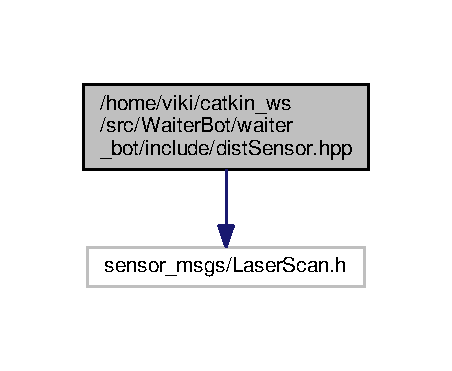
\includegraphics[width=217pt]{distSensor_8hpp__incl}
\end{center}
\end{figure}
This graph shows which files directly or indirectly include this file\+:
\nopagebreak
\begin{figure}[H]
\begin{center}
\leavevmode
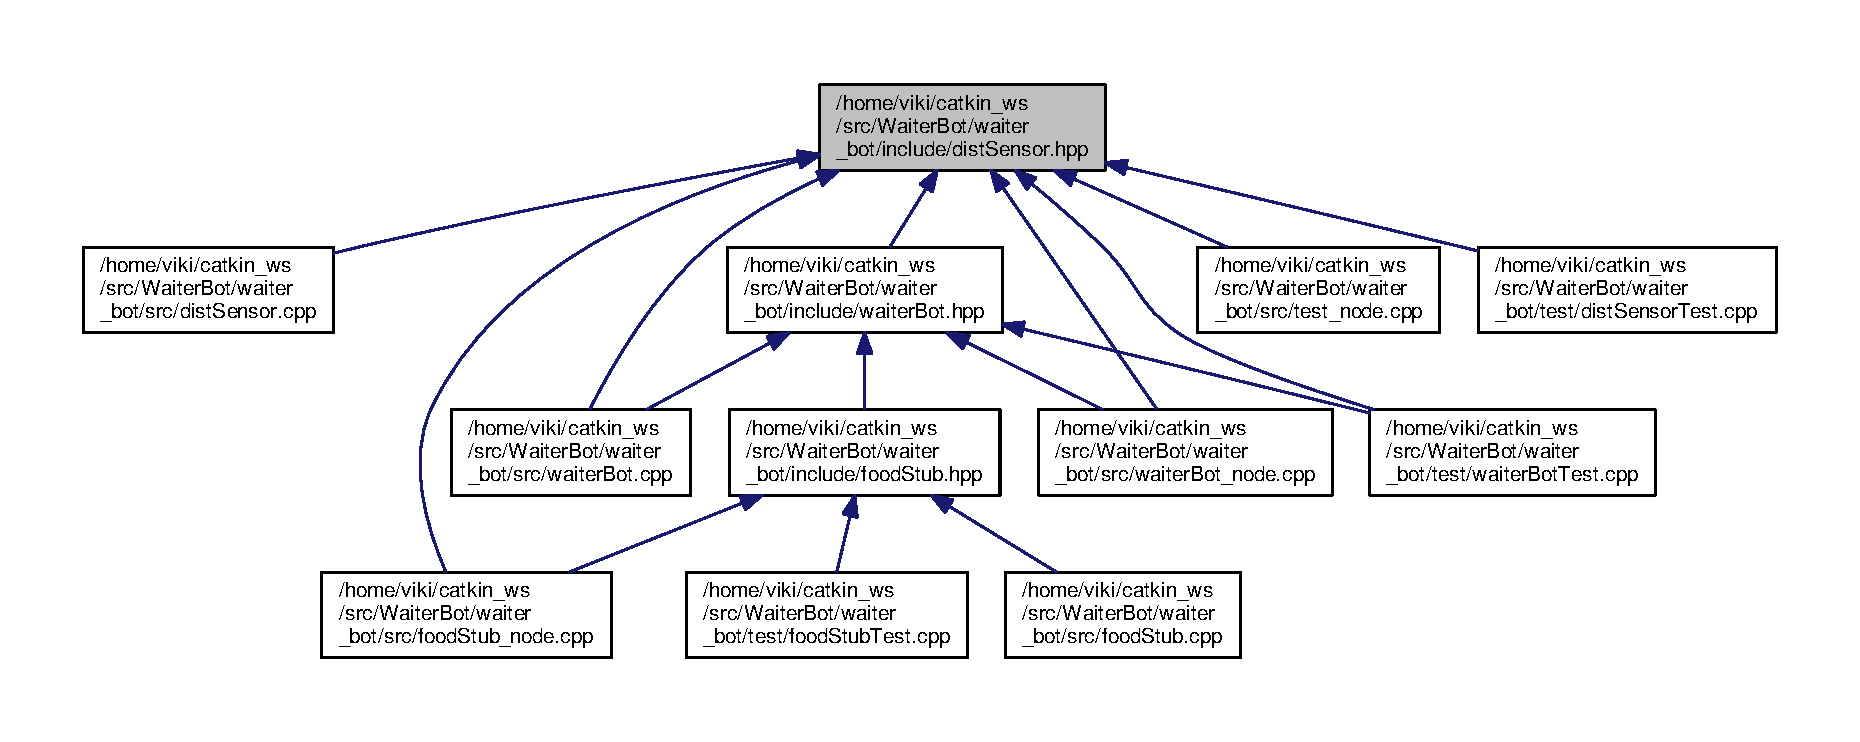
\includegraphics[width=350pt]{distSensor_8hpp__dep__incl}
\end{center}
\end{figure}
\subsection*{Classes}
\begin{DoxyCompactItemize}
\item 
class \hyperlink{classdistSensor}{dist\+Sensor}
\begin{DoxyCompactList}\small\item\em A distance sensor Class. \end{DoxyCompactList}\end{DoxyCompactItemize}


\subsection{Detailed Description}
This is the \char`\"{}.\+hpp\char`\"{} file for the \hyperlink{classdistSensor}{dist\+Sensor} Class. 

\begin{DoxyAuthor}{Author}
Ruben Acevedo
\end{DoxyAuthor}
\begin{DoxyCopyright}{Copyright}
\mbox{[}2017\mbox{]} Ruben Acevedo
\end{DoxyCopyright}
This file will define the methods and attributes of the \hyperlink{classdistSensor}{dist\+Sensor} Class 
\hypertarget{foodStub_8hpp}{}\section{/home/viki/catkin\+\_\+ws/src/\+Waiter\+Bot/waiter\+\_\+bot/include/food\+Stub.hpp File Reference}
\label{foodStub_8hpp}\index{/home/viki/catkin\+\_\+ws/src/\+Waiter\+Bot/waiter\+\_\+bot/include/food\+Stub.\+hpp@{/home/viki/catkin\+\_\+ws/src/\+Waiter\+Bot/waiter\+\_\+bot/include/food\+Stub.\+hpp}}


This is the \char`\"{}.\+hpp\char`\"{} file for the food stub Class.  


{\ttfamily \#include $<$std\+\_\+msgs/\+Float32.\+h$>$}\\*
{\ttfamily \#include \char`\"{}waiter\+Bot.\+hpp\char`\"{}}\\*
Include dependency graph for food\+Stub.\+hpp\+:
\nopagebreak
\begin{figure}[H]
\begin{center}
\leavevmode
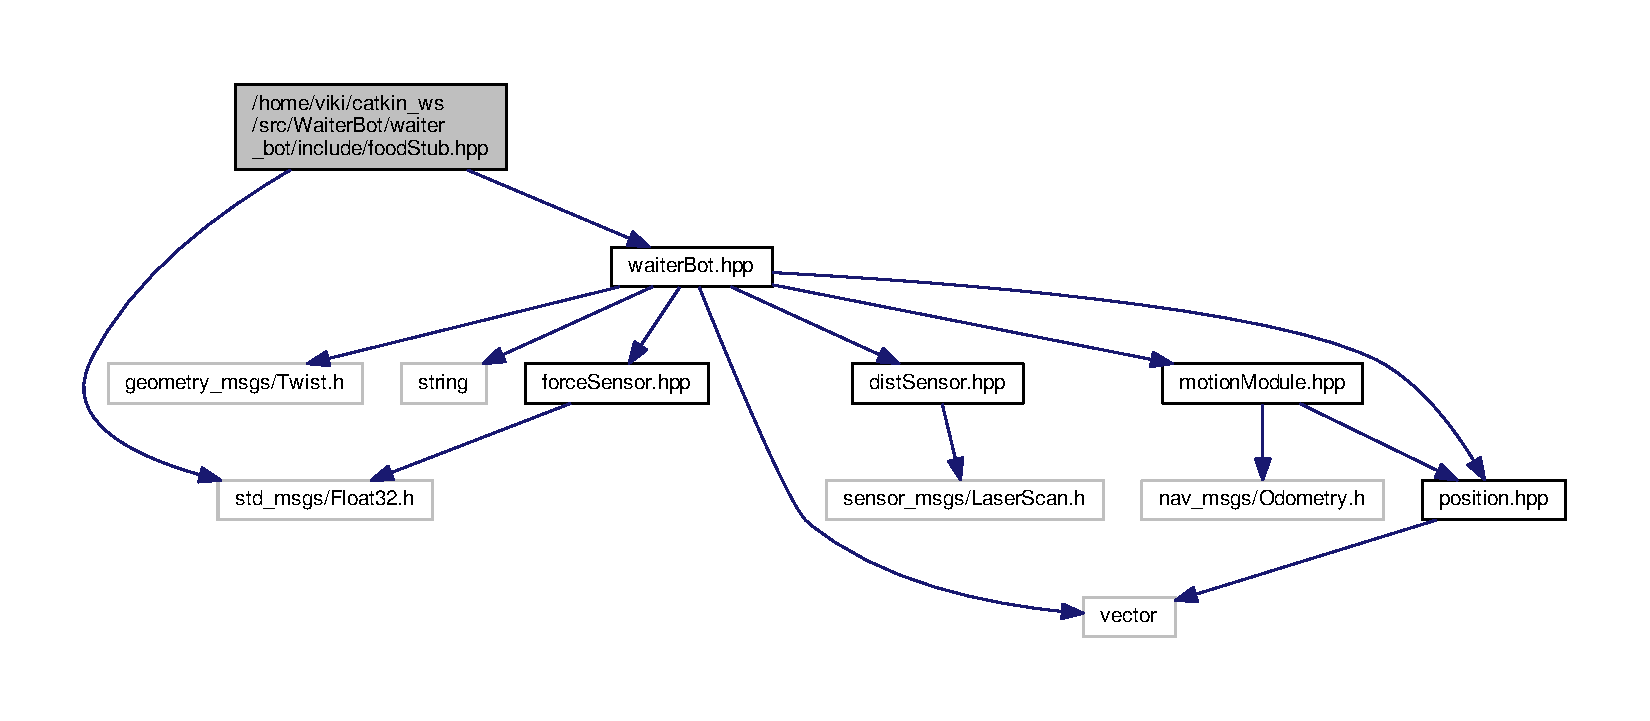
\includegraphics[width=350pt]{foodStub_8hpp__incl}
\end{center}
\end{figure}
This graph shows which files directly or indirectly include this file\+:
\nopagebreak
\begin{figure}[H]
\begin{center}
\leavevmode
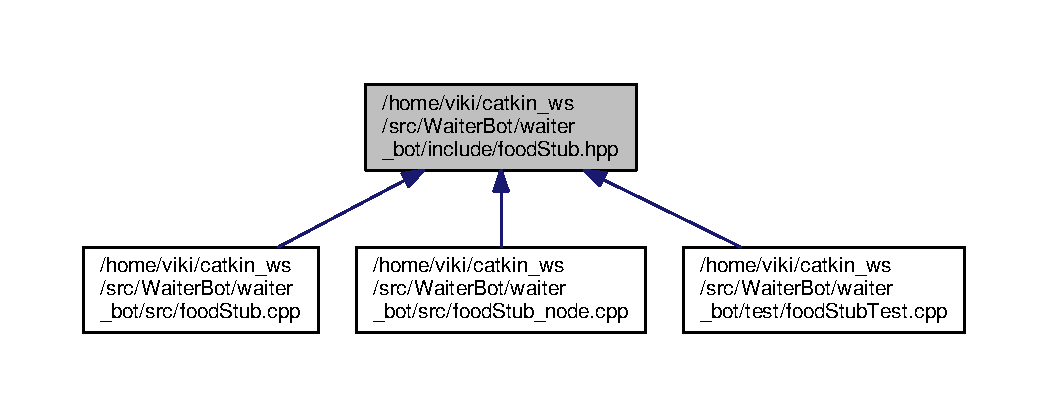
\includegraphics[width=350pt]{foodStub_8hpp__dep__incl}
\end{center}
\end{figure}
\subsection*{Classes}
\begin{DoxyCompactItemize}
\item 
class \hyperlink{classfoodStub}{food\+Stub}
\begin{DoxyCompactList}\small\item\em A food stub Class. \end{DoxyCompactList}\end{DoxyCompactItemize}


\subsection{Detailed Description}
This is the \char`\"{}.\+hpp\char`\"{} file for the food stub Class. 

\begin{DoxyAuthor}{Author}
Ruben Acevedo
\end{DoxyAuthor}
\begin{DoxyCopyright}{Copyright}
\mbox{[}2017\mbox{]} Ruben Acevedo
\end{DoxyCopyright}
This file will define the methods and attributes of the food stub Class 
\hypertarget{forceSensor_8hpp}{}\section{/home/viki/catkin\+\_\+ws/src/\+Waiter\+Bot/waiter\+\_\+bot/include/force\+Sensor.hpp File Reference}
\label{forceSensor_8hpp}\index{/home/viki/catkin\+\_\+ws/src/\+Waiter\+Bot/waiter\+\_\+bot/include/force\+Sensor.\+hpp@{/home/viki/catkin\+\_\+ws/src/\+Waiter\+Bot/waiter\+\_\+bot/include/force\+Sensor.\+hpp}}


This is the \char`\"{}.\+hpp\char`\"{} file for the force sensor Class.  


{\ttfamily \#include $<$std\+\_\+msgs/\+Float32.\+h$>$}\\*
Include dependency graph for force\+Sensor.\+hpp\+:
\nopagebreak
\begin{figure}[H]
\begin{center}
\leavevmode
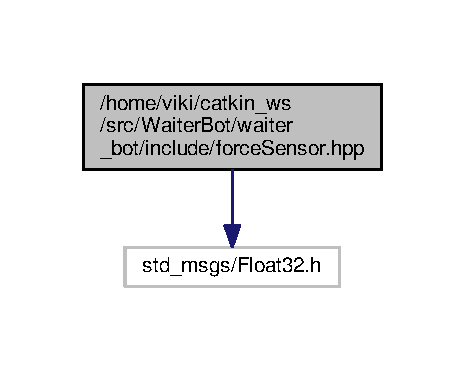
\includegraphics[width=223pt]{forceSensor_8hpp__incl}
\end{center}
\end{figure}
This graph shows which files directly or indirectly include this file\+:
\nopagebreak
\begin{figure}[H]
\begin{center}
\leavevmode
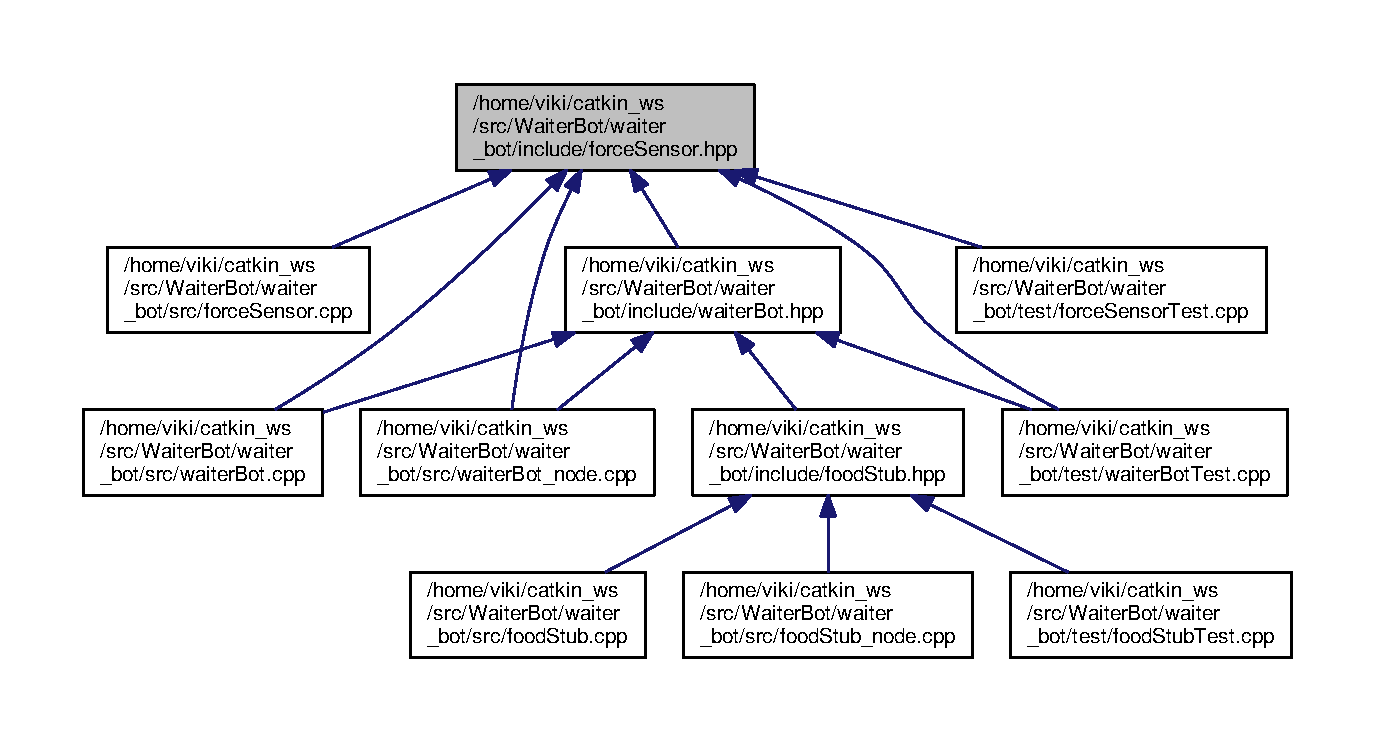
\includegraphics[width=350pt]{forceSensor_8hpp__dep__incl}
\end{center}
\end{figure}
\subsection*{Classes}
\begin{DoxyCompactItemize}
\item 
class \hyperlink{classforceSensor}{force\+Sensor}
\begin{DoxyCompactList}\small\item\em A force sensor Class. \end{DoxyCompactList}\end{DoxyCompactItemize}


\subsection{Detailed Description}
This is the \char`\"{}.\+hpp\char`\"{} file for the force sensor Class. 

\begin{DoxyAuthor}{Author}
Ruben Acevedo
\end{DoxyAuthor}
\begin{DoxyCopyright}{Copyright}
\mbox{[}2017\mbox{]} Ruben Acevedo
\end{DoxyCopyright}
This file will define the methods and attributes of the force sensor Class 
\hypertarget{motionModule_8hpp}{}\section{/home/viki/catkin\+\_\+ws/src/\+Waiter\+Bot/waiter\+\_\+bot/include/motion\+Module.hpp File Reference}
\label{motionModule_8hpp}\index{/home/viki/catkin\+\_\+ws/src/\+Waiter\+Bot/waiter\+\_\+bot/include/motion\+Module.\+hpp@{/home/viki/catkin\+\_\+ws/src/\+Waiter\+Bot/waiter\+\_\+bot/include/motion\+Module.\+hpp}}


This is the \char`\"{}.\+hpp\char`\"{} file for the \hyperlink{classmotionModule}{motion\+Module} Class.  


{\ttfamily \#include $<$nav\+\_\+msgs/\+Odometry.\+h$>$}\\*
{\ttfamily \#include \char`\"{}position.\+hpp\char`\"{}}\\*
Include dependency graph for motion\+Module.\+hpp\+:
\nopagebreak
\begin{figure}[H]
\begin{center}
\leavevmode
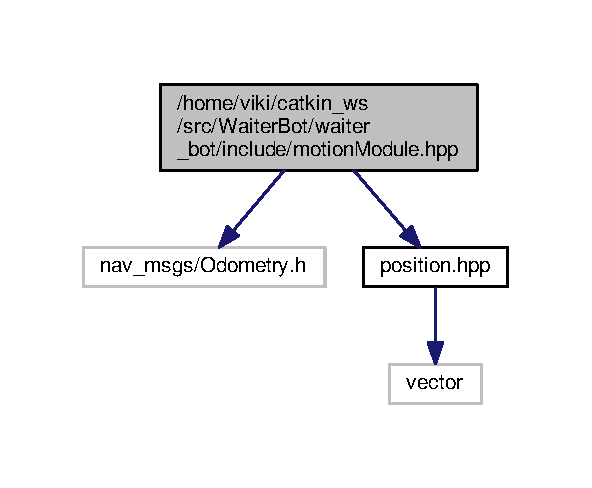
\includegraphics[width=284pt]{motionModule_8hpp__incl}
\end{center}
\end{figure}
This graph shows which files directly or indirectly include this file\+:
\nopagebreak
\begin{figure}[H]
\begin{center}
\leavevmode
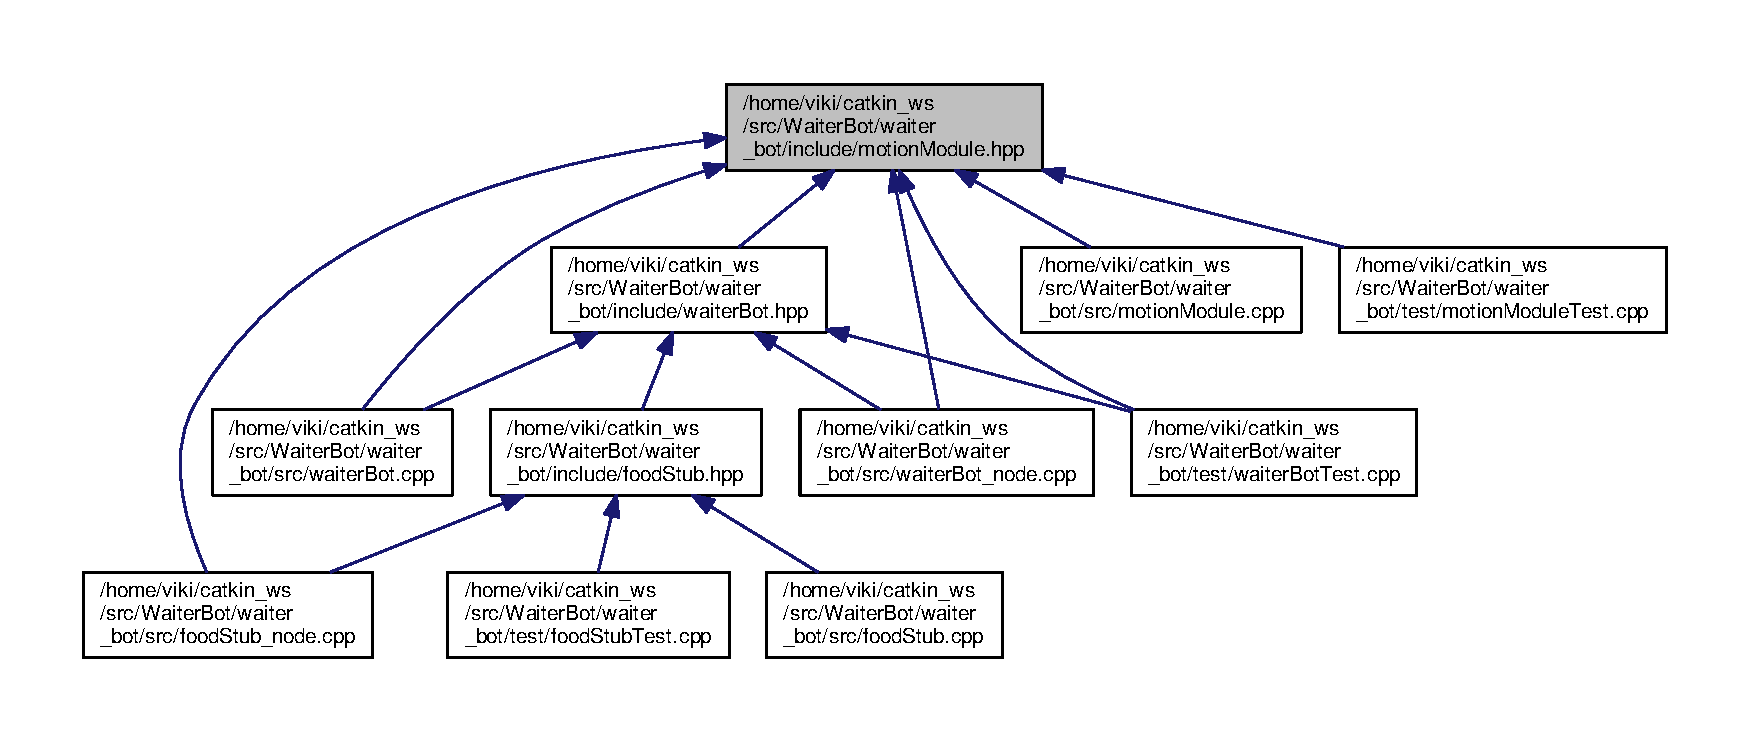
\includegraphics[width=350pt]{motionModule_8hpp__dep__incl}
\end{center}
\end{figure}
\subsection*{Classes}
\begin{DoxyCompactItemize}
\item 
class \hyperlink{classmotionModule}{motion\+Module}
\begin{DoxyCompactList}\small\item\em A motion module Class. \end{DoxyCompactList}\end{DoxyCompactItemize}


\subsection{Detailed Description}
This is the \char`\"{}.\+hpp\char`\"{} file for the \hyperlink{classmotionModule}{motion\+Module} Class. 

\begin{DoxyAuthor}{Author}
Ruben Acevedo
\end{DoxyAuthor}
\begin{DoxyCopyright}{Copyright}
\mbox{[}2017\mbox{]} Ruben Acevedo
\end{DoxyCopyright}
This file will define the methods and attributes of the \hyperlink{classmotionModule}{motion\+Module} Class 
\hypertarget{position_8hpp}{}\section{/home/viki/catkin\+\_\+ws/src/\+Waiter\+Bot/waiter\+\_\+bot/include/position.hpp File Reference}
\label{position_8hpp}\index{/home/viki/catkin\+\_\+ws/src/\+Waiter\+Bot/waiter\+\_\+bot/include/position.\+hpp@{/home/viki/catkin\+\_\+ws/src/\+Waiter\+Bot/waiter\+\_\+bot/include/position.\+hpp}}


This is the \char`\"{}.\+hpp\char`\"{} file for the position Class.  


{\ttfamily \#include $<$vector$>$}\\*
Include dependency graph for position.\+hpp\+:
\nopagebreak
\begin{figure}[H]
\begin{center}
\leavevmode
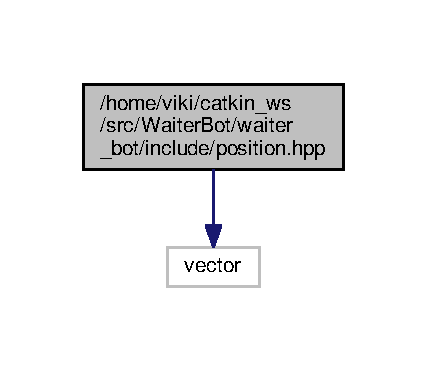
\includegraphics[width=205pt]{position_8hpp__incl}
\end{center}
\end{figure}
This graph shows which files directly or indirectly include this file\+:
\nopagebreak
\begin{figure}[H]
\begin{center}
\leavevmode
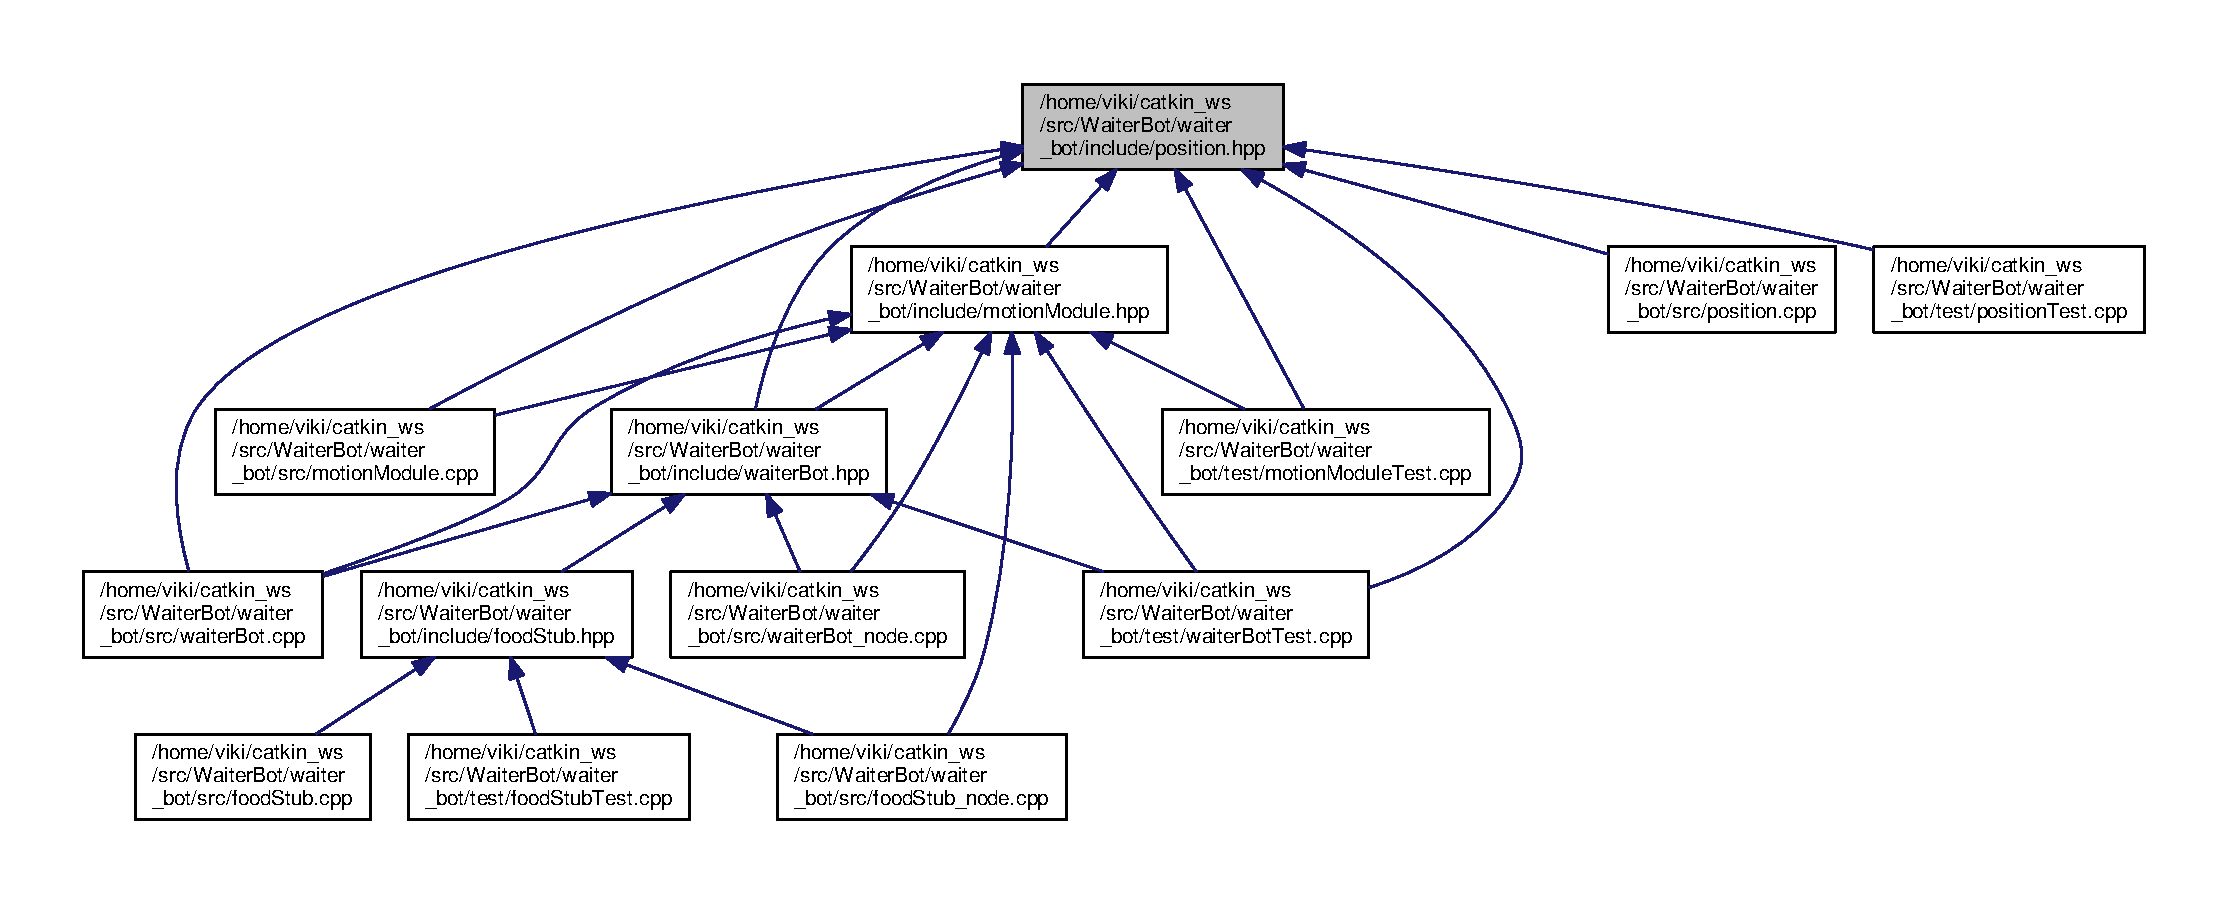
\includegraphics[width=350pt]{position_8hpp__dep__incl}
\end{center}
\end{figure}
\subsection*{Classes}
\begin{DoxyCompactItemize}
\item 
class \hyperlink{classposition}{position}
\begin{DoxyCompactList}\small\item\em A Position Class. \end{DoxyCompactList}\end{DoxyCompactItemize}


\subsection{Detailed Description}
This is the \char`\"{}.\+hpp\char`\"{} file for the position Class. 

\begin{DoxyAuthor}{Author}
Ruben Acevedo
\end{DoxyAuthor}
\begin{DoxyCopyright}{Copyright}
\mbox{[}2017\mbox{]} Ruben Acevedo
\end{DoxyCopyright}
This file will define the methods and attributes of the position Class 
\hypertarget{waiterBot_8hpp}{}\section{/home/viki/catkin\+\_\+ws/src/\+Waiter\+Bot/waiter\+\_\+bot/include/waiter\+Bot.hpp File Reference}
\label{waiterBot_8hpp}\index{/home/viki/catkin\+\_\+ws/src/\+Waiter\+Bot/waiter\+\_\+bot/include/waiter\+Bot.\+hpp@{/home/viki/catkin\+\_\+ws/src/\+Waiter\+Bot/waiter\+\_\+bot/include/waiter\+Bot.\+hpp}}


This is the \char`\"{}.\+hpp\char`\"{} file for the \hyperlink{classwaiterBot}{waiter\+Bot} Class.  


{\ttfamily \#include $<$geometry\+\_\+msgs/\+Twist.\+h$>$}\\*
{\ttfamily \#include $<$string$>$}\\*
{\ttfamily \#include $<$vector$>$}\\*
{\ttfamily \#include \char`\"{}dist\+Sensor.\+hpp\char`\"{}}\\*
{\ttfamily \#include \char`\"{}motion\+Module.\+hpp\char`\"{}}\\*
{\ttfamily \#include \char`\"{}force\+Sensor.\+hpp\char`\"{}}\\*
{\ttfamily \#include \char`\"{}position.\+hpp\char`\"{}}\\*
Include dependency graph for waiter\+Bot.\+hpp\+:
\nopagebreak
\begin{figure}[H]
\begin{center}
\leavevmode
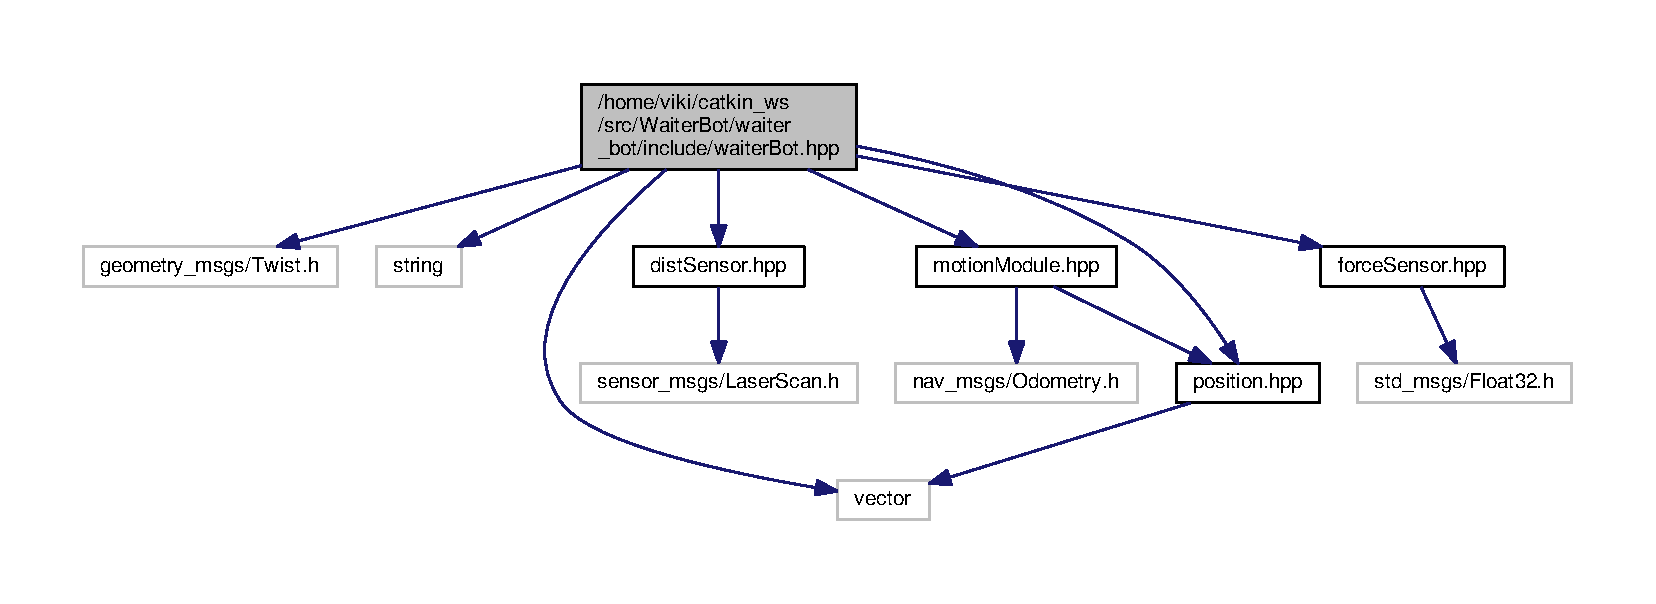
\includegraphics[width=350pt]{waiterBot_8hpp__incl}
\end{center}
\end{figure}
This graph shows which files directly or indirectly include this file\+:
\nopagebreak
\begin{figure}[H]
\begin{center}
\leavevmode
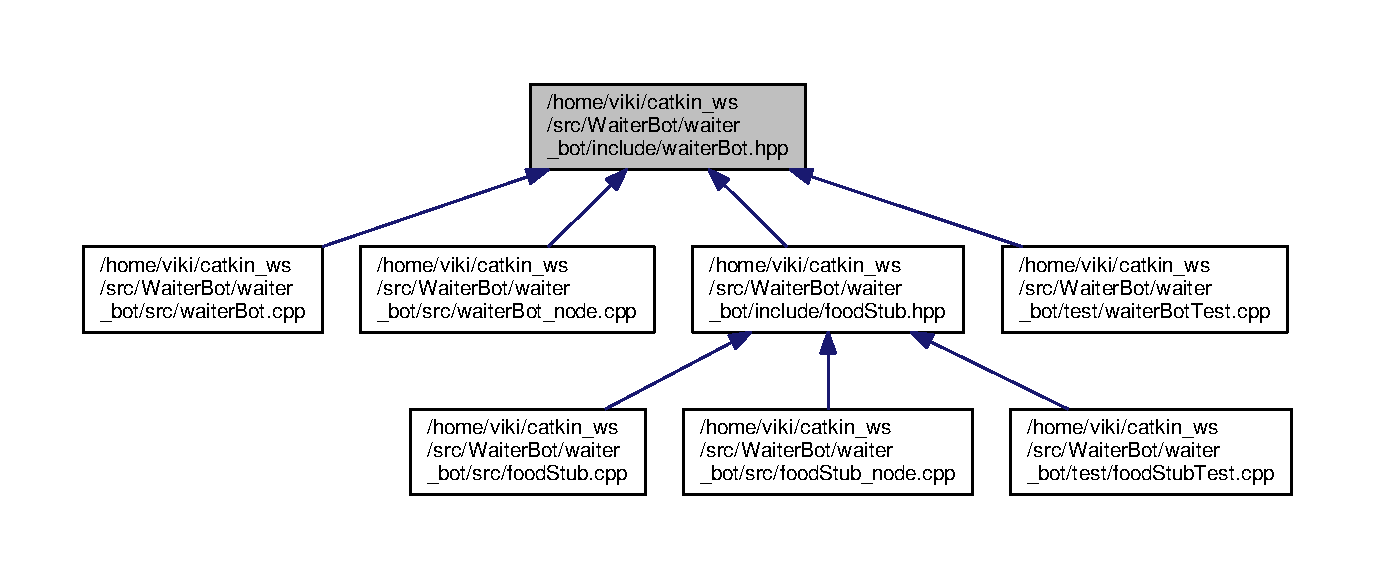
\includegraphics[width=350pt]{waiterBot_8hpp__dep__incl}
\end{center}
\end{figure}
\subsection*{Classes}
\begin{DoxyCompactItemize}
\item 
class \hyperlink{classwaiterBot}{waiter\+Bot}
\begin{DoxyCompactList}\small\item\em A \hyperlink{classwaiterBot}{waiter\+Bot} Class. \end{DoxyCompactList}\end{DoxyCompactItemize}


\subsection{Detailed Description}
This is the \char`\"{}.\+hpp\char`\"{} file for the \hyperlink{classwaiterBot}{waiter\+Bot} Class. 

\begin{DoxyAuthor}{Author}
Ruben Acevedo
\end{DoxyAuthor}
\begin{DoxyCopyright}{Copyright}
\mbox{[}2017\mbox{]} Ruben Acevedo
\end{DoxyCopyright}
This file will define the methods and attributes of the \hyperlink{classwaiterBot}{waiter\+Bot} Class 
\hypertarget{distSensor_8cpp}{}\section{/home/viki/catkin\+\_\+ws/src/\+Waiter\+Bot/waiter\+\_\+bot/src/dist\+Sensor.cpp File Reference}
\label{distSensor_8cpp}\index{/home/viki/catkin\+\_\+ws/src/\+Waiter\+Bot/waiter\+\_\+bot/src/dist\+Sensor.\+cpp@{/home/viki/catkin\+\_\+ws/src/\+Waiter\+Bot/waiter\+\_\+bot/src/dist\+Sensor.\+cpp}}


This is the \char`\"{}.\+cpp\char`\"{} file for the \hyperlink{classdistSensor}{dist\+Sensor} Class.  


{\ttfamily \#include $<$sensor\+\_\+msgs/\+Laser\+Scan.\+h$>$}\\*
{\ttfamily \#include $<$ros/ros.\+h$>$}\\*
{\ttfamily \#include \char`\"{}dist\+Sensor.\+hpp\char`\"{}}\\*
Include dependency graph for dist\+Sensor.\+cpp\+:
\nopagebreak
\begin{figure}[H]
\begin{center}
\leavevmode
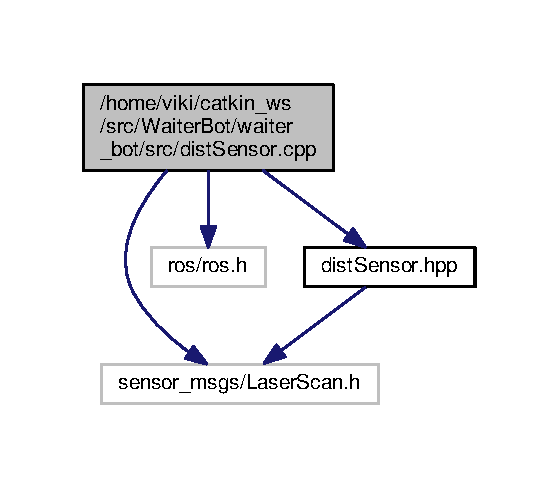
\includegraphics[width=268pt]{distSensor_8cpp__incl}
\end{center}
\end{figure}


\subsection{Detailed Description}
This is the \char`\"{}.\+cpp\char`\"{} file for the \hyperlink{classdistSensor}{dist\+Sensor} Class. 

\begin{DoxyAuthor}{Author}
Ruben Acevedo
\end{DoxyAuthor}
\begin{DoxyCopyright}{Copyright}
\mbox{[}2017\mbox{]} Ruben Acevedo
\end{DoxyCopyright}
This file implements the methods and attributes of the \hyperlink{classdistSensor}{dist\+Sensor} Class. 
\hypertarget{foodStub_8cpp}{}\section{/home/viki/catkin\+\_\+ws/src/\+Waiter\+Bot/waiter\+\_\+bot/src/food\+Stub.cpp File Reference}
\label{foodStub_8cpp}\index{/home/viki/catkin\+\_\+ws/src/\+Waiter\+Bot/waiter\+\_\+bot/src/food\+Stub.\+cpp@{/home/viki/catkin\+\_\+ws/src/\+Waiter\+Bot/waiter\+\_\+bot/src/food\+Stub.\+cpp}}


This is the \char`\"{}.\+cpp\char`\"{} file for the food stub Class.  


{\ttfamily \#include $<$std\+\_\+msgs/\+Float32.\+h$>$}\\*
{\ttfamily \#include $<$ros/ros.\+h$>$}\\*
{\ttfamily \#include \char`\"{}food\+Stub.\+hpp\char`\"{}}\\*
Include dependency graph for food\+Stub.\+cpp\+:
\nopagebreak
\begin{figure}[H]
\begin{center}
\leavevmode
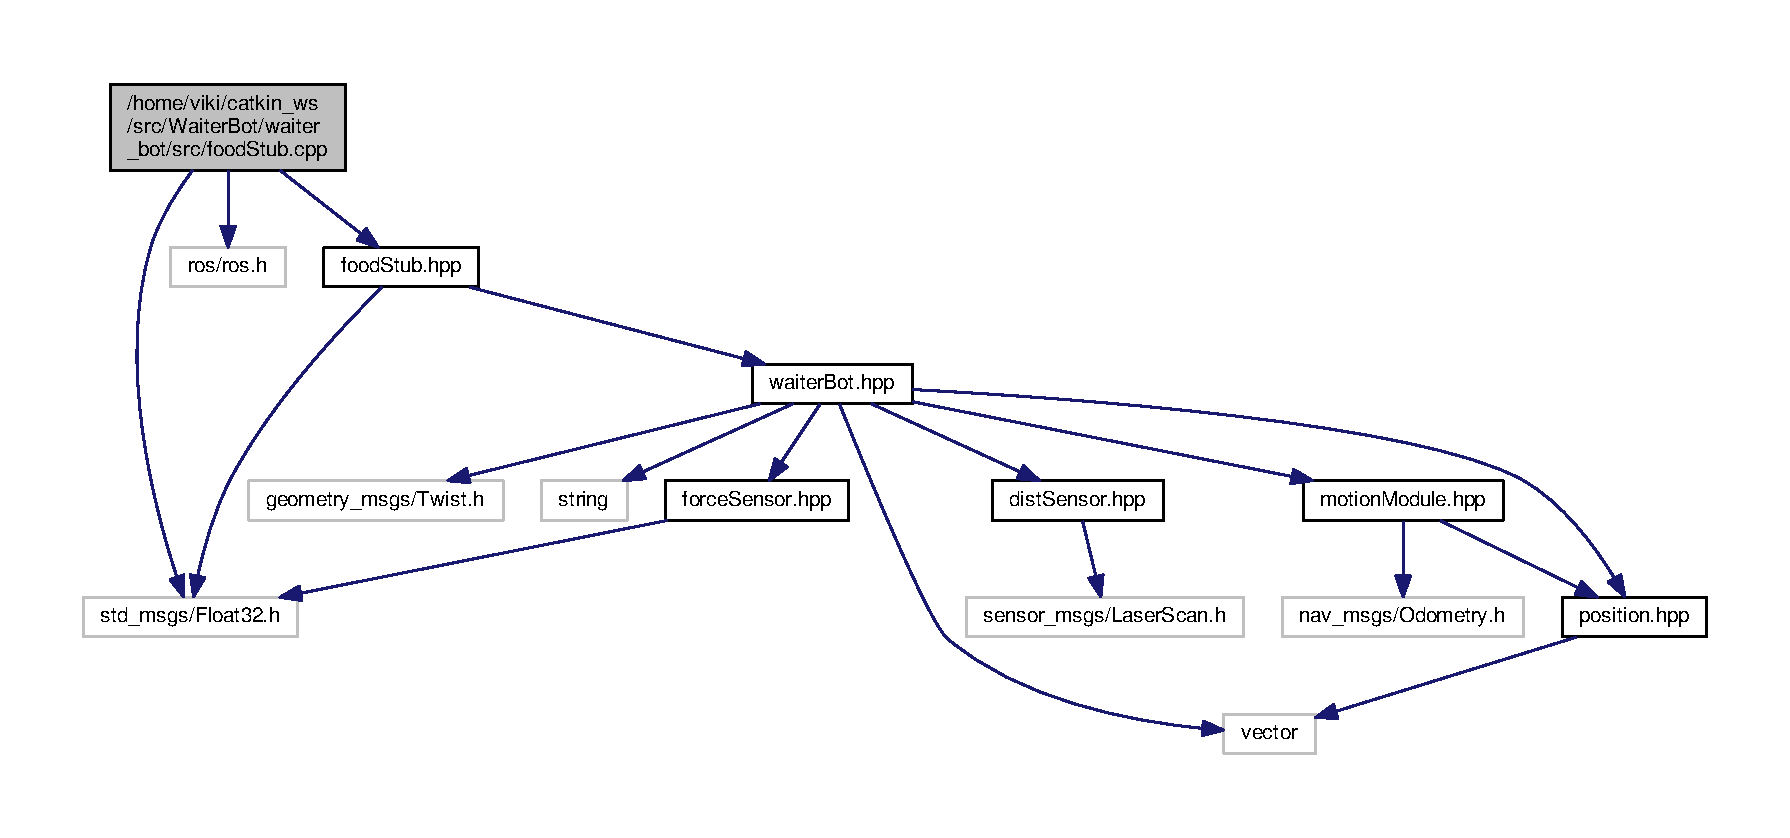
\includegraphics[width=350pt]{foodStub_8cpp__incl}
\end{center}
\end{figure}


\subsection{Detailed Description}
This is the \char`\"{}.\+cpp\char`\"{} file for the food stub Class. 

\begin{DoxyAuthor}{Author}
Ruben Acevedo
\end{DoxyAuthor}
\begin{DoxyCopyright}{Copyright}
\mbox{[}2017\mbox{]} Ruben Acevedo
\end{DoxyCopyright}
This file implements the methods and attributes of the food stub Class. 
\hypertarget{foodStub__node_8cpp}{}\section{/home/viki/catkin\+\_\+ws/src/\+Waiter\+Bot/waiter\+\_\+bot/src/food\+Stub\+\_\+node.cpp File Reference}
\label{foodStub__node_8cpp}\index{/home/viki/catkin\+\_\+ws/src/\+Waiter\+Bot/waiter\+\_\+bot/src/food\+Stub\+\_\+node.\+cpp@{/home/viki/catkin\+\_\+ws/src/\+Waiter\+Bot/waiter\+\_\+bot/src/food\+Stub\+\_\+node.\+cpp}}


This is the \char`\"{}.\+cpp\char`\"{} file for the \hyperlink{classfoodStub}{food\+Stub} node.  


{\ttfamily \#include $<$std\+\_\+msgs/\+Float32.\+h$>$}\\*
{\ttfamily \#include $<$ros/ros.\+h$>$}\\*
{\ttfamily \#include \char`\"{}dist\+Sensor.\+hpp\char`\"{}}\\*
{\ttfamily \#include \char`\"{}motion\+Module.\+hpp\char`\"{}}\\*
{\ttfamily \#include \char`\"{}food\+Stub.\+hpp\char`\"{}}\\*
Include dependency graph for food\+Stub\+\_\+node.\+cpp\+:
\nopagebreak
\begin{figure}[H]
\begin{center}
\leavevmode
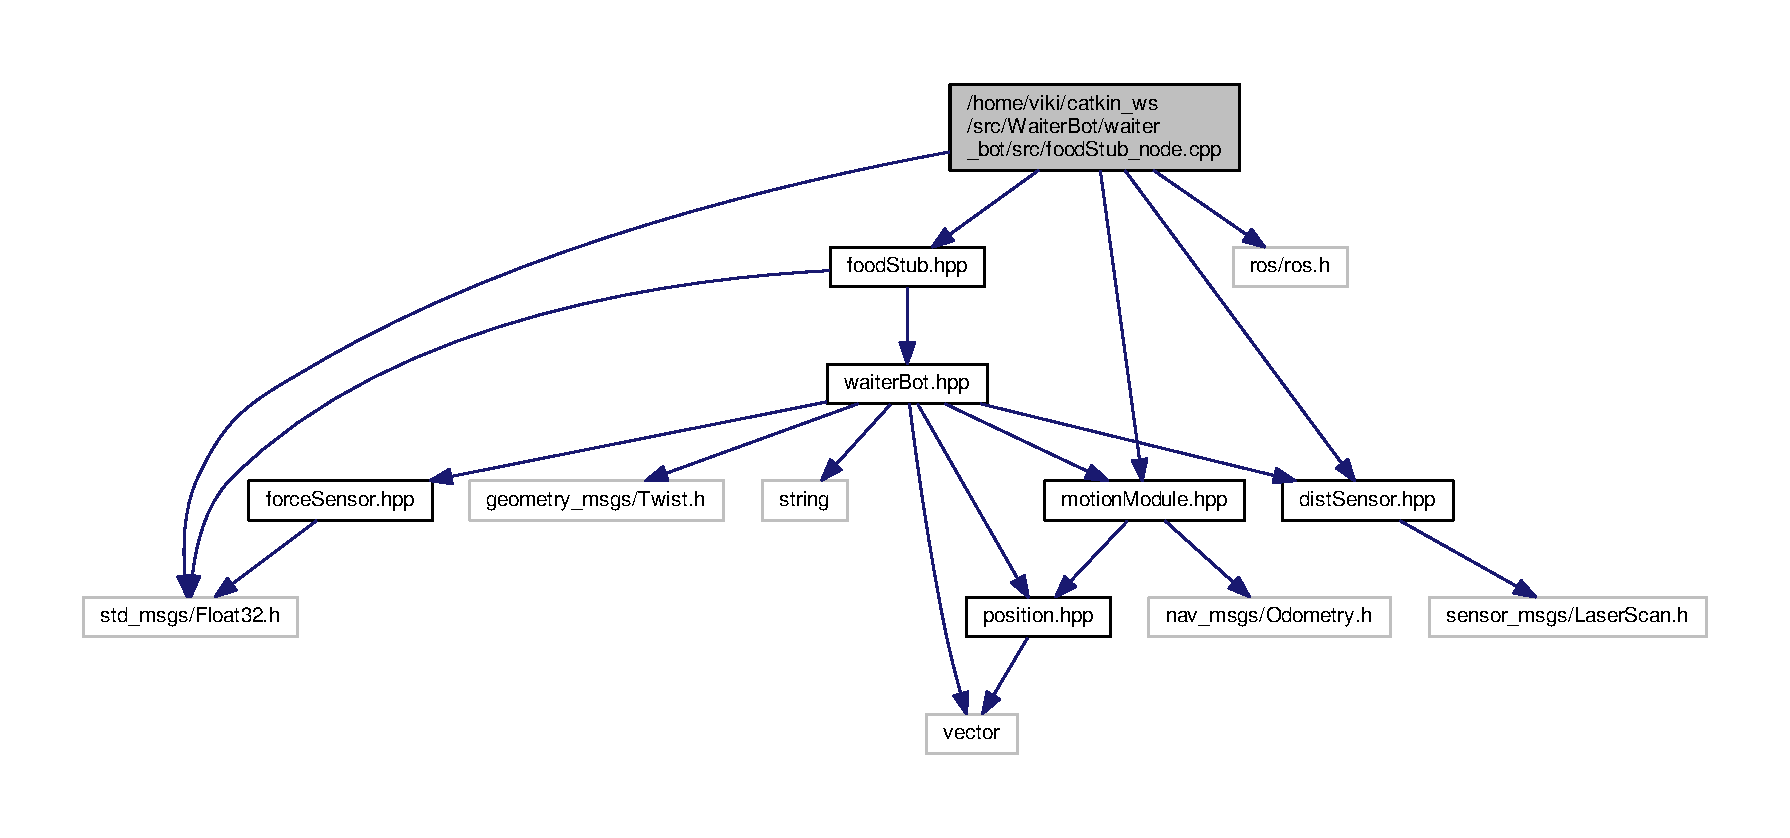
\includegraphics[width=350pt]{foodStub__node_8cpp__incl}
\end{center}
\end{figure}
\subsection*{Functions}
\begin{DoxyCompactItemize}
\item 
int \hyperlink{foodStub__node_8cpp_a3c04138a5bfe5d72780bb7e82a18e627}{main} (int argc, char $\ast$$\ast$argv)
\begin{DoxyCompactList}\small\item\em This node runs the food stub When the robot is in target location 1 it publishes 25N of food. Everytime it reaches a target location it reduces the food by 1/5 the original value. Everytime the robot is stopped it also reduces the food by 1/5 the original value. This node publishes std\+\_\+msgs\+::\+Float32 messages to the force topic. This node subscribes to the /odom topic. \end{DoxyCompactList}\end{DoxyCompactItemize}


\subsection{Detailed Description}
This is the \char`\"{}.\+cpp\char`\"{} file for the \hyperlink{classfoodStub}{food\+Stub} node. 

\begin{DoxyAuthor}{Author}
Ruben Acevedo
\end{DoxyAuthor}
\begin{DoxyCopyright}{Copyright}
\mbox{[}2017\mbox{]} Ruben Acevedo 
\end{DoxyCopyright}


\subsection{Function Documentation}
\index{food\+Stub\+\_\+node.\+cpp@{food\+Stub\+\_\+node.\+cpp}!main@{main}}
\index{main@{main}!food\+Stub\+\_\+node.\+cpp@{food\+Stub\+\_\+node.\+cpp}}
\subsubsection[{\texorpdfstring{main(int argc, char $\ast$$\ast$argv)}{main(int argc, char **argv)}}]{\setlength{\rightskip}{0pt plus 5cm}int main (
\begin{DoxyParamCaption}
\item[{int}]{argc, }
\item[{char $\ast$$\ast$}]{argv}
\end{DoxyParamCaption}
)}\hypertarget{foodStub__node_8cpp_a3c04138a5bfe5d72780bb7e82a18e627}{}\label{foodStub__node_8cpp_a3c04138a5bfe5d72780bb7e82a18e627}


This node runs the food stub When the robot is in target location 1 it publishes 25N of food. Everytime it reaches a target location it reduces the food by 1/5 the original value. Everytime the robot is stopped it also reduces the food by 1/5 the original value. This node publishes std\+\_\+msgs\+::\+Float32 messages to the force topic. This node subscribes to the /odom topic. 

M\+IT License

Copyright 2017 Ruben Acevedo

Permission is hereby granted, free of charge, to any person obtaining a copy of this software and associated documentation files (the \char`\"{}\+Software\char`\"{}), to deal in the Software without restriction, including without limitation the rights to use, copy, modify, merge, publish, distribute, sublicense, and/or sell copies of the Software, and to permit persons to whom the Software is furnished to do so, subject to the following conditions\+:

The above copyright notice and this permission notice shall be included in all copies or substantial portions of the Software. T\+HE S\+O\+F\+T\+W\+A\+RE IS P\+R\+O\+V\+I\+D\+ED \char`\"{}\+A\+S I\+S\char`\"{}, W\+I\+T\+H\+O\+UT W\+A\+R\+R\+A\+N\+TY OF A\+NY K\+I\+ND, E\+X\+P\+R\+E\+SS OR I\+M\+P\+L\+I\+ED, I\+N\+C\+L\+U\+D\+I\+NG B\+UT N\+OT L\+I\+M\+I\+T\+ED TO T\+HE W\+A\+R\+R\+A\+N\+T\+I\+ES OF M\+E\+R\+C\+H\+A\+N\+T\+A\+B\+I\+L\+I\+TY, F\+I\+T\+N\+E\+SS F\+OR A P\+A\+R\+T\+I\+C\+U\+L\+AR P\+U\+R\+P\+O\+SE A\+ND N\+O\+N\+I\+N\+F\+R\+I\+N\+G\+E\+M\+E\+NT. IN NO E\+V\+E\+NT S\+H\+A\+LL T\+HE A\+U\+T\+H\+O\+RS OR C\+O\+P\+Y\+R\+I\+G\+HT H\+O\+L\+D\+E\+RS BE L\+I\+A\+B\+LE F\+OR A\+NY C\+L\+A\+IM, D\+A\+M\+A\+G\+ES OR O\+T\+H\+ER L\+I\+A\+B\+I\+L\+I\+TY, W\+H\+E\+T\+H\+ER IN AN A\+C\+T\+I\+ON OF C\+O\+N\+T\+R\+A\+CT, T\+O\+RT OR O\+T\+H\+E\+R\+W\+I\+SE, A\+R\+I\+S\+I\+NG F\+R\+OM, O\+UT OF OR IN C\+O\+N\+N\+E\+C\+T\+I\+ON W\+I\+TH T\+HE S\+O\+F\+T\+W\+A\+RE OR T\+HE U\+SE OR O\+T\+H\+ER D\+E\+A\+L\+I\+N\+GS IN T\+HE S\+O\+F\+T\+W\+A\+RE. © 2017 Git\+Hub, Inc. subscribe the \hyperlink{classmotionModule}{motion\+Module} to the /odom topic

subscribe the \hyperlink{classdistSensor}{dist\+Sensor} to the /scan topic

publish the the food weight to the force topic the weights are gstd\+\_\+msgs\+::\+Float32 message type
\hypertarget{forceSensor_8cpp}{}\section{/home/viki/catkin\+\_\+ws/src/\+Waiter\+Bot/waiter\+\_\+bot/src/force\+Sensor.cpp File Reference}
\label{forceSensor_8cpp}\index{/home/viki/catkin\+\_\+ws/src/\+Waiter\+Bot/waiter\+\_\+bot/src/force\+Sensor.\+cpp@{/home/viki/catkin\+\_\+ws/src/\+Waiter\+Bot/waiter\+\_\+bot/src/force\+Sensor.\+cpp}}


This is the \char`\"{}.\+cpp\char`\"{} file for the force sensor Class.  


{\ttfamily \#include $<$std\+\_\+msgs/\+Float32.\+h$>$}\\*
{\ttfamily \#include $<$ros/ros.\+h$>$}\\*
{\ttfamily \#include \char`\"{}force\+Sensor.\+hpp\char`\"{}}\\*
Include dependency graph for force\+Sensor.\+cpp\+:
\nopagebreak
\begin{figure}[H]
\begin{center}
\leavevmode
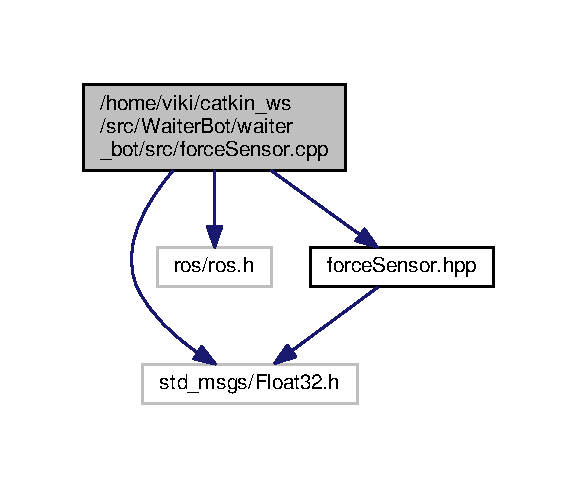
\includegraphics[width=277pt]{forceSensor_8cpp__incl}
\end{center}
\end{figure}


\subsection{Detailed Description}
This is the \char`\"{}.\+cpp\char`\"{} file for the force sensor Class. 

\begin{DoxyAuthor}{Author}
Ruben Acevedo
\end{DoxyAuthor}
\begin{DoxyCopyright}{Copyright}
\mbox{[}2017\mbox{]} Ruben Acevedo
\end{DoxyCopyright}
This file implements the methods and attributes of the force sensor Class. 
\hypertarget{motionModule_8cpp}{}\section{/home/viki/catkin\+\_\+ws/src/\+Waiter\+Bot/waiter\+\_\+bot/src/motion\+Module.cpp File Reference}
\label{motionModule_8cpp}\index{/home/viki/catkin\+\_\+ws/src/\+Waiter\+Bot/waiter\+\_\+bot/src/motion\+Module.\+cpp@{/home/viki/catkin\+\_\+ws/src/\+Waiter\+Bot/waiter\+\_\+bot/src/motion\+Module.\+cpp}}


This is the \char`\"{}.\+cpp\char`\"{} file for the \hyperlink{classmotionModule}{motion\+Module} Class.  


{\ttfamily \#include $<$nav\+\_\+msgs/\+Odometry.\+h$>$}\\*
{\ttfamily \#include $<$tf/transform\+\_\+broadcaster.\+h$>$}\\*
{\ttfamily \#include $<$math.\+h$>$}\\*
{\ttfamily \#include $<$ros/ros.\+h$>$}\\*
{\ttfamily \#include \char`\"{}position.\+hpp\char`\"{}}\\*
{\ttfamily \#include \char`\"{}motion\+Module.\+hpp\char`\"{}}\\*
Include dependency graph for motion\+Module.\+cpp\+:
\nopagebreak
\begin{figure}[H]
\begin{center}
\leavevmode
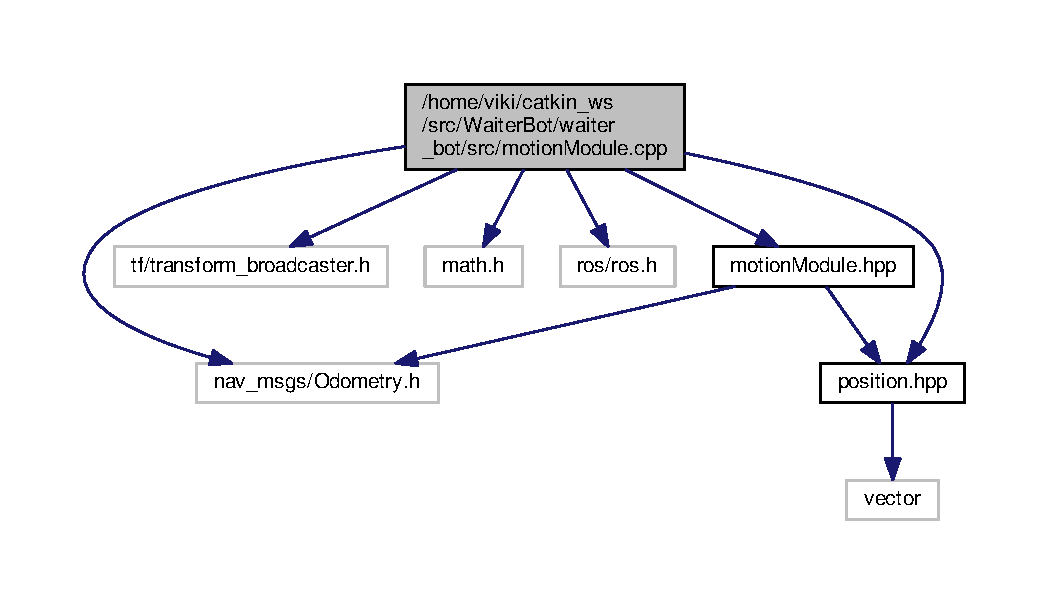
\includegraphics[width=350pt]{motionModule_8cpp__incl}
\end{center}
\end{figure}


\subsection{Detailed Description}
This is the \char`\"{}.\+cpp\char`\"{} file for the \hyperlink{classmotionModule}{motion\+Module} Class. 

\begin{DoxyAuthor}{Author}
Ruben Acevedo
\end{DoxyAuthor}
\begin{DoxyCopyright}{Copyright}
\mbox{[}2017\mbox{]} Ruben Acevedo
\end{DoxyCopyright}
This file implements the methods and attributes of the \hyperlink{classmotionModule}{motion\+Module} Class. 
\hypertarget{position_8cpp}{}\section{/home/viki/catkin\+\_\+ws/src/\+Waiter\+Bot/waiter\+\_\+bot/src/position.cpp File Reference}
\label{position_8cpp}\index{/home/viki/catkin\+\_\+ws/src/\+Waiter\+Bot/waiter\+\_\+bot/src/position.\+cpp@{/home/viki/catkin\+\_\+ws/src/\+Waiter\+Bot/waiter\+\_\+bot/src/position.\+cpp}}


This is the \char`\"{}.\+cpp\char`\"{} file for the position Class.  


{\ttfamily \#include $<$vector$>$}\\*
{\ttfamily \#include \char`\"{}position.\+hpp\char`\"{}}\\*
Include dependency graph for position.\+cpp\+:
\nopagebreak
\begin{figure}[H]
\begin{center}
\leavevmode
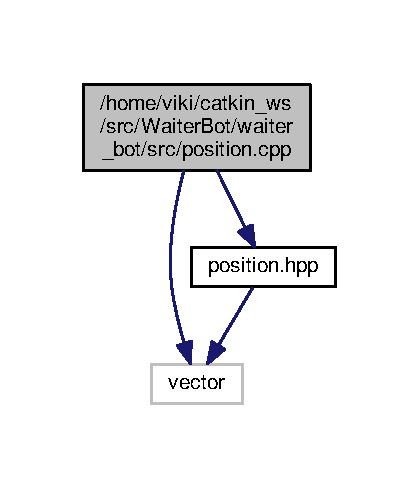
\includegraphics[width=201pt]{position_8cpp__incl}
\end{center}
\end{figure}


\subsection{Detailed Description}
This is the \char`\"{}.\+cpp\char`\"{} file for the position Class. 

\begin{DoxyAuthor}{Author}
Ruben Acevedo
\end{DoxyAuthor}
\begin{DoxyCopyright}{Copyright}
\mbox{[}2017\mbox{]} Ruben Acevedo
\end{DoxyCopyright}
This file implements the methods and attributes of the position Class. 
\hypertarget{test__node_8cpp}{}\section{/home/viki/catkin\+\_\+ws/src/\+Waiter\+Bot/waiter\+\_\+bot/src/test\+\_\+node.cpp File Reference}
\label{test__node_8cpp}\index{/home/viki/catkin\+\_\+ws/src/\+Waiter\+Bot/waiter\+\_\+bot/src/test\+\_\+node.\+cpp@{/home/viki/catkin\+\_\+ws/src/\+Waiter\+Bot/waiter\+\_\+bot/src/test\+\_\+node.\+cpp}}


This is the \char`\"{}.\+cpp\char`\"{} file for the test node.  


{\ttfamily \#include $<$sensor\+\_\+msgs/\+Laser\+Scan.\+h$>$}\\*
{\ttfamily \#include $<$nav\+\_\+msgs/\+Odometry.\+h$>$}\\*
{\ttfamily \#include $<$ros/ros.\+h$>$}\\*
{\ttfamily \#include \char`\"{}dist\+Sensor.\+hpp\char`\"{}}\\*
Include dependency graph for test\+\_\+node.\+cpp\+:
\nopagebreak
\begin{figure}[H]
\begin{center}
\leavevmode
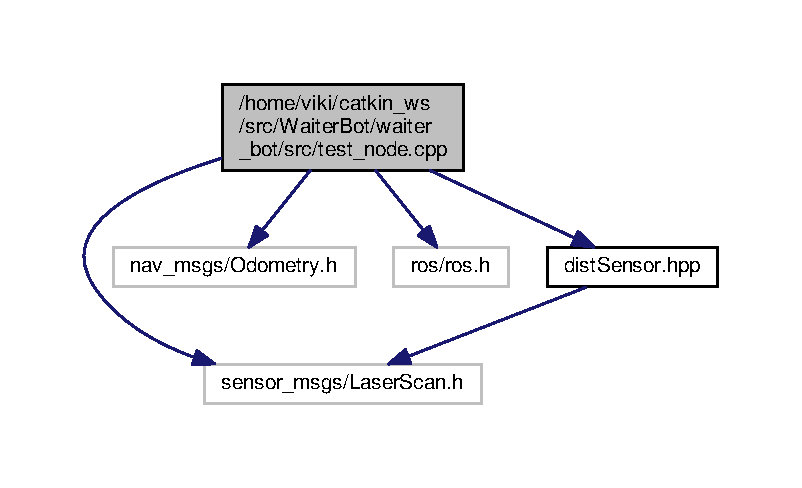
\includegraphics[width=350pt]{test__node_8cpp__incl}
\end{center}
\end{figure}
\subsection*{Functions}
\begin{DoxyCompactItemize}
\item 
int \hyperlink{test__node_8cpp_a3c04138a5bfe5d72780bb7e82a18e627}{main} (int argc, char $\ast$$\ast$argv)
\begin{DoxyCompactList}\small\item\em This node run is used for testing The node publishes sensor\+\_\+msgs\+::\+Laser\+Scan data This node also publishes nav\+\_\+msgs\+::\+Odometry data. \end{DoxyCompactList}\end{DoxyCompactItemize}


\subsection{Detailed Description}
This is the \char`\"{}.\+cpp\char`\"{} file for the test node. 

\begin{DoxyAuthor}{Author}
Ruben Acevedo
\end{DoxyAuthor}
\begin{DoxyCopyright}{Copyright}
\mbox{[}2017\mbox{]} Ruben Acevedo 
\end{DoxyCopyright}


\subsection{Function Documentation}
\index{test\+\_\+node.\+cpp@{test\+\_\+node.\+cpp}!main@{main}}
\index{main@{main}!test\+\_\+node.\+cpp@{test\+\_\+node.\+cpp}}
\subsubsection[{\texorpdfstring{main(int argc, char $\ast$$\ast$argv)}{main(int argc, char **argv)}}]{\setlength{\rightskip}{0pt plus 5cm}int main (
\begin{DoxyParamCaption}
\item[{int}]{argc, }
\item[{char $\ast$$\ast$}]{argv}
\end{DoxyParamCaption}
)}\hypertarget{test__node_8cpp_a3c04138a5bfe5d72780bb7e82a18e627}{}\label{test__node_8cpp_a3c04138a5bfe5d72780bb7e82a18e627}


This node run is used for testing The node publishes sensor\+\_\+msgs\+::\+Laser\+Scan data This node also publishes nav\+\_\+msgs\+::\+Odometry data. 

M\+IT License

Copyright 2017 Ruben Acevedo

Permission is hereby granted, free of charge, to any person obtaining a copy of this software and associated documentation files (the \char`\"{}\+Software\char`\"{}), to deal in the Software without restriction, including without limitation the rights to use, copy, modify, merge, publish, distribute, sublicense, and/or sell copies of the Software, and to permit persons to whom the Software is furnished to do so, subject to the following conditions\+:

The above copyright notice and this permission notice shall be included in all copies or substantial portions of the Software. T\+HE S\+O\+F\+T\+W\+A\+RE IS P\+R\+O\+V\+I\+D\+ED \char`\"{}\+A\+S I\+S\char`\"{}, W\+I\+T\+H\+O\+UT W\+A\+R\+R\+A\+N\+TY OF A\+NY K\+I\+ND, E\+X\+P\+R\+E\+SS OR I\+M\+P\+L\+I\+ED, I\+N\+C\+L\+U\+D\+I\+NG B\+UT N\+OT L\+I\+M\+I\+T\+ED TO T\+HE W\+A\+R\+R\+A\+N\+T\+I\+ES OF M\+E\+R\+C\+H\+A\+N\+T\+A\+B\+I\+L\+I\+TY, F\+I\+T\+N\+E\+SS F\+OR A P\+A\+R\+T\+I\+C\+U\+L\+AR P\+U\+R\+P\+O\+SE A\+ND N\+O\+N\+I\+N\+F\+R\+I\+N\+G\+E\+M\+E\+NT. IN NO E\+V\+E\+NT S\+H\+A\+LL T\+HE A\+U\+T\+H\+O\+RS OR C\+O\+P\+Y\+R\+I\+G\+HT H\+O\+L\+D\+E\+RS BE L\+I\+A\+B\+LE F\+OR A\+NY C\+L\+A\+IM, D\+A\+M\+A\+G\+ES OR O\+T\+H\+ER L\+I\+A\+B\+I\+L\+I\+TY, W\+H\+E\+T\+H\+ER IN AN A\+C\+T\+I\+ON OF C\+O\+N\+T\+R\+A\+CT, T\+O\+RT OR O\+T\+H\+E\+R\+W\+I\+SE, A\+R\+I\+S\+I\+NG F\+R\+OM, O\+UT OF OR IN C\+O\+N\+N\+E\+C\+T\+I\+ON W\+I\+TH T\+HE S\+O\+F\+T\+W\+A\+RE OR T\+HE U\+SE OR O\+T\+H\+ER D\+E\+A\+L\+I\+N\+GS IN T\+HE S\+O\+F\+T\+W\+A\+RE. © 2017 Git\+Hub, Inc. This is creating a sensor\+\_\+msgs\+::\+Laser\+Scan publisher to test the \hyperlink{classdistSensor}{dist\+Sensor} class and waiter\+Bot\+\_\+node

This is creating a nav\+\_\+msgs\+::\+Odometry publisher to test the waiter\+Bot\+\_\+node

This sets the robot location to target location 2;
\hypertarget{waiterBot_8cpp}{}\section{/home/viki/catkin\+\_\+ws/src/\+Waiter\+Bot/waiter\+\_\+bot/src/waiter\+Bot.cpp File Reference}
\label{waiterBot_8cpp}\index{/home/viki/catkin\+\_\+ws/src/\+Waiter\+Bot/waiter\+\_\+bot/src/waiter\+Bot.\+cpp@{/home/viki/catkin\+\_\+ws/src/\+Waiter\+Bot/waiter\+\_\+bot/src/waiter\+Bot.\+cpp}}


This is the \char`\"{}.\+cpp\char`\"{} file for the \hyperlink{classwaiterBot}{waiter\+Bot} Class.  


{\ttfamily \#include \char`\"{}waiter\+Bot.\+hpp\char`\"{}}\\*
{\ttfamily \#include $<$ros/ros.\+h$>$}\\*
{\ttfamily \#include $<$math.\+h$>$}\\*
{\ttfamily \#include $<$geometry\+\_\+msgs/\+Twist.\+h$>$}\\*
{\ttfamily \#include $<$string$>$}\\*
{\ttfamily \#include $<$vector$>$}\\*
{\ttfamily \#include \char`\"{}dist\+Sensor.\+hpp\char`\"{}}\\*
{\ttfamily \#include \char`\"{}motion\+Module.\+hpp\char`\"{}}\\*
{\ttfamily \#include \char`\"{}force\+Sensor.\+hpp\char`\"{}}\\*
{\ttfamily \#include \char`\"{}position.\+hpp\char`\"{}}\\*
Include dependency graph for waiter\+Bot.\+cpp\+:
\nopagebreak
\begin{figure}[H]
\begin{center}
\leavevmode
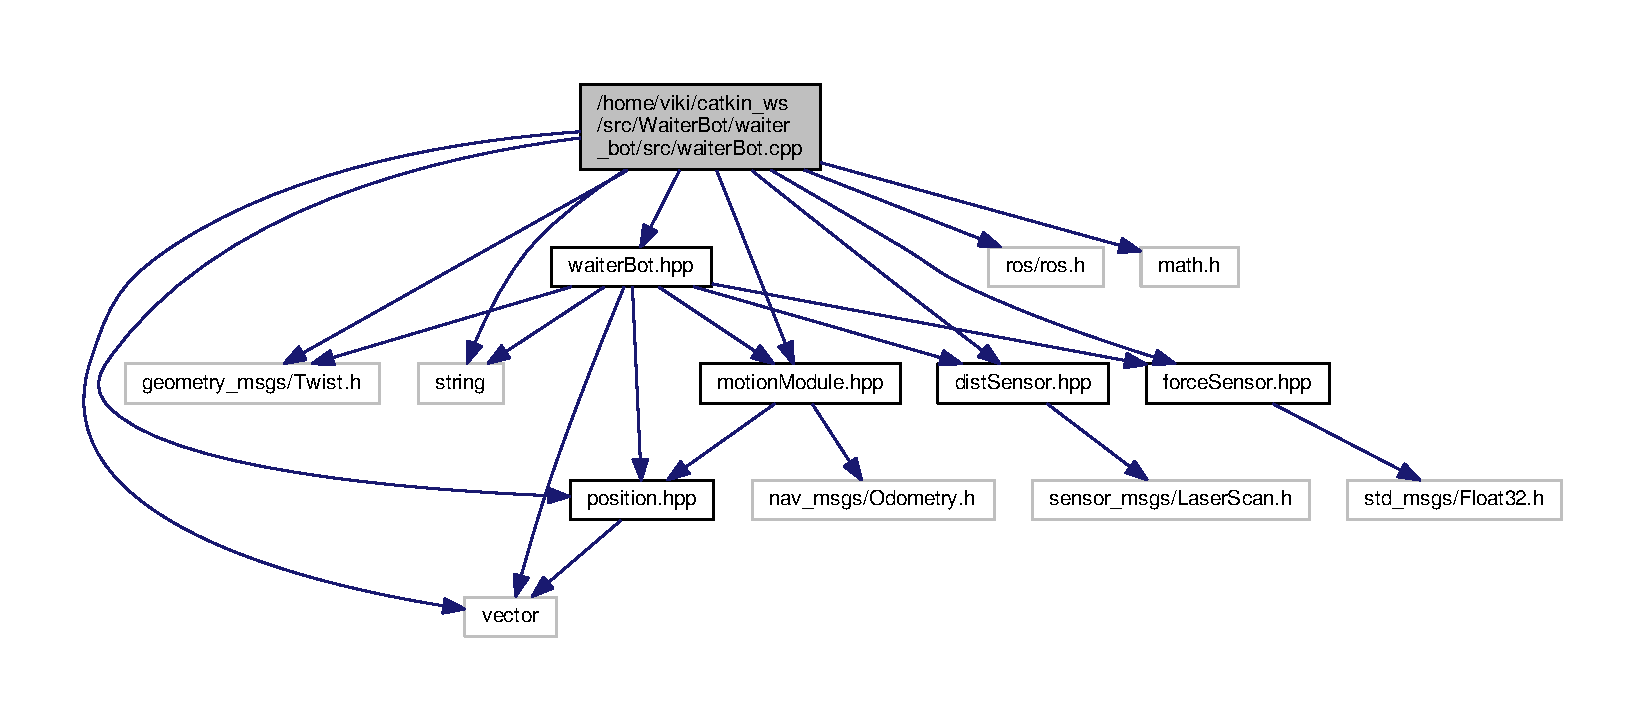
\includegraphics[width=350pt]{waiterBot_8cpp__incl}
\end{center}
\end{figure}


\subsection{Detailed Description}
This is the \char`\"{}.\+cpp\char`\"{} file for the \hyperlink{classwaiterBot}{waiter\+Bot} Class. 

\begin{DoxyAuthor}{Author}
Ruben Acevedo
\end{DoxyAuthor}
\begin{DoxyCopyright}{Copyright}
\mbox{[}2017\mbox{]} Ruben Acevedo
\end{DoxyCopyright}
This file implements the methods and attributes of the \hyperlink{classwaiterBot}{waiter\+Bot} Class. 
\hypertarget{waiterBot__node_8cpp}{}\section{/home/viki/catkin\+\_\+ws/src/\+Waiter\+Bot/waiter\+\_\+bot/src/waiter\+Bot\+\_\+node.cpp File Reference}
\label{waiterBot__node_8cpp}\index{/home/viki/catkin\+\_\+ws/src/\+Waiter\+Bot/waiter\+\_\+bot/src/waiter\+Bot\+\_\+node.\+cpp@{/home/viki/catkin\+\_\+ws/src/\+Waiter\+Bot/waiter\+\_\+bot/src/waiter\+Bot\+\_\+node.\+cpp}}


This is the \char`\"{}.\+cpp\char`\"{} file for the \hyperlink{classwaiterBot}{waiter\+Bot} node.  


{\ttfamily \#include $<$ros/ros.\+h$>$}\\*
{\ttfamily \#include $<$geometry\+\_\+msgs/\+Twist.\+h$>$}\\*
{\ttfamily \#include $<$std\+\_\+msgs/\+String.\+h$>$}\\*
{\ttfamily \#include $<$sstream$>$}\\*
{\ttfamily \#include \char`\"{}waiter\+Bot.\+hpp\char`\"{}}\\*
{\ttfamily \#include \char`\"{}dist\+Sensor.\+hpp\char`\"{}}\\*
{\ttfamily \#include \char`\"{}motion\+Module.\+hpp\char`\"{}}\\*
{\ttfamily \#include \char`\"{}force\+Sensor.\+hpp\char`\"{}}\\*
Include dependency graph for waiter\+Bot\+\_\+node.\+cpp\+:
\nopagebreak
\begin{figure}[H]
\begin{center}
\leavevmode
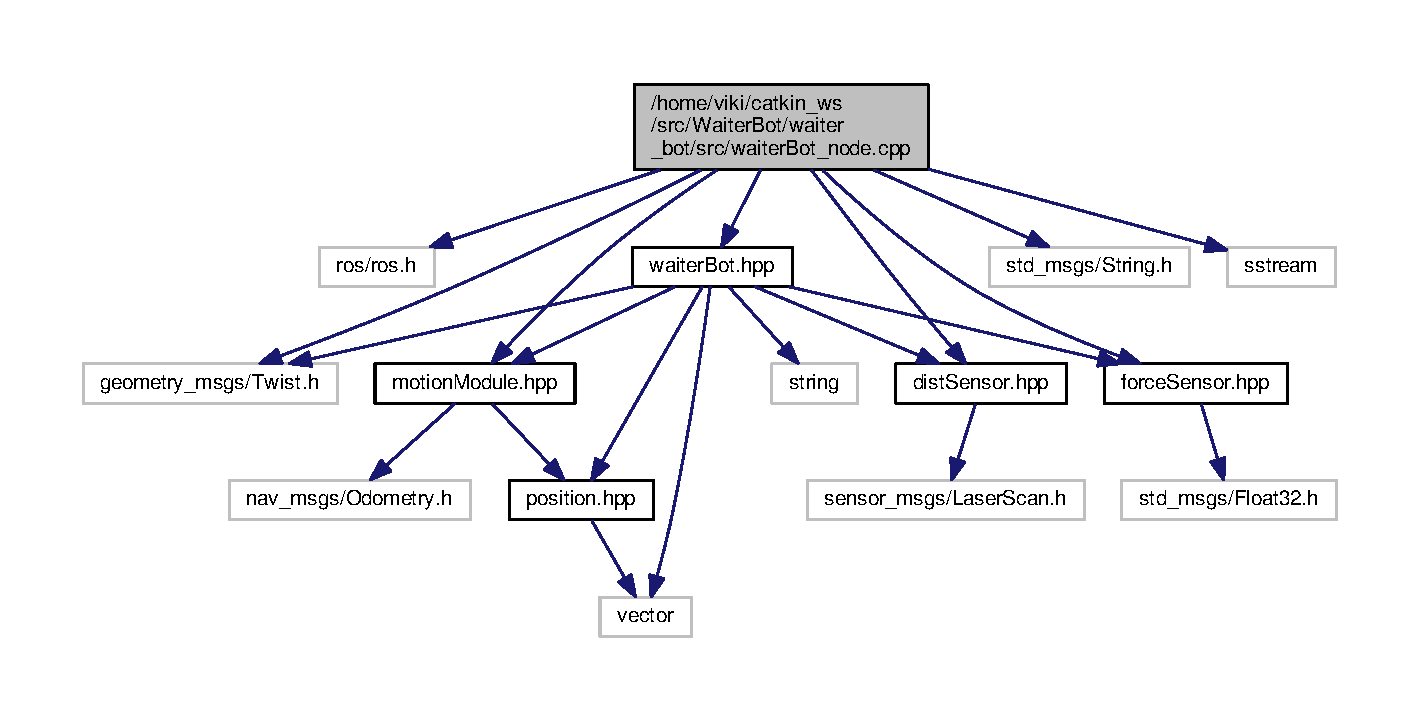
\includegraphics[width=350pt]{waiterBot__node_8cpp__incl}
\end{center}
\end{figure}
\subsection*{Functions}
\begin{DoxyCompactItemize}
\item 
int \hyperlink{waiterBot__node_8cpp_a3c04138a5bfe5d72780bb7e82a18e627}{main} (int argc, char $\ast$$\ast$argv)
\begin{DoxyCompactList}\small\item\em This node run the \hyperlink{classwaiterBot}{waiter\+Bot} Demo The robot moves to its target location, stoping every time there is an obstical, and it retruns to the food/drink pick up location only once it has no more food It publishes geometry\+\_\+msgs\+::\+Twist messages from the \char`\"{}/mobile\+\_\+base/commands/velocity\char`\"{} topic It subscribes to the the \char`\"{}/scan\char`\"{}, \char`\"{}force\char`\"{}, \char`\"{}/odom\char`\"{} topic. \end{DoxyCompactList}\end{DoxyCompactItemize}


\subsection{Detailed Description}
This is the \char`\"{}.\+cpp\char`\"{} file for the \hyperlink{classwaiterBot}{waiter\+Bot} node. 

\begin{DoxyAuthor}{Author}
Ruben Acevedo
\end{DoxyAuthor}
\begin{DoxyCopyright}{Copyright}
\mbox{[}2017\mbox{]} Ruben Acevedo 
\end{DoxyCopyright}


\subsection{Function Documentation}
\index{waiter\+Bot\+\_\+node.\+cpp@{waiter\+Bot\+\_\+node.\+cpp}!main@{main}}
\index{main@{main}!waiter\+Bot\+\_\+node.\+cpp@{waiter\+Bot\+\_\+node.\+cpp}}
\subsubsection[{\texorpdfstring{main(int argc, char $\ast$$\ast$argv)}{main(int argc, char **argv)}}]{\setlength{\rightskip}{0pt plus 5cm}int main (
\begin{DoxyParamCaption}
\item[{int}]{argc, }
\item[{char $\ast$$\ast$}]{argv}
\end{DoxyParamCaption}
)}\hypertarget{waiterBot__node_8cpp_a3c04138a5bfe5d72780bb7e82a18e627}{}\label{waiterBot__node_8cpp_a3c04138a5bfe5d72780bb7e82a18e627}


This node run the \hyperlink{classwaiterBot}{waiter\+Bot} Demo The robot moves to its target location, stoping every time there is an obstical, and it retruns to the food/drink pick up location only once it has no more food It publishes geometry\+\_\+msgs\+::\+Twist messages from the \char`\"{}/mobile\+\_\+base/commands/velocity\char`\"{} topic It subscribes to the the \char`\"{}/scan\char`\"{}, \char`\"{}force\char`\"{}, \char`\"{}/odom\char`\"{} topic. 

M\+IT License

Copyright 2017 Ruben Acevedo

Permission is hereby granted, free of charge, to any person obtaining a copy of this software and associated documentation files (the \char`\"{}\+Software\char`\"{}), to deal in the Software without restriction, including without limitation the rights to use, copy, modify, merge, publish, distribute, sublicense, and/or sell copies of the Software, and to permit persons to whom the Software is furnished to do so, subject to the following conditions\+:

The above copyright notice and this permission notice shall be included in all copies or substantial portions of the Software. T\+HE S\+O\+F\+T\+W\+A\+RE IS P\+R\+O\+V\+I\+D\+ED \char`\"{}\+A\+S I\+S\char`\"{}, W\+I\+T\+H\+O\+UT W\+A\+R\+R\+A\+N\+TY OF A\+NY K\+I\+ND, E\+X\+P\+R\+E\+SS OR I\+M\+P\+L\+I\+ED, I\+N\+C\+L\+U\+D\+I\+NG B\+UT N\+OT L\+I\+M\+I\+T\+ED TO T\+HE W\+A\+R\+R\+A\+N\+T\+I\+ES OF M\+E\+R\+C\+H\+A\+N\+T\+A\+B\+I\+L\+I\+TY, F\+I\+T\+N\+E\+SS F\+OR A P\+A\+R\+T\+I\+C\+U\+L\+AR P\+U\+R\+P\+O\+SE A\+ND N\+O\+N\+I\+N\+F\+R\+I\+N\+G\+E\+M\+E\+NT. IN NO E\+V\+E\+NT S\+H\+A\+LL T\+HE A\+U\+T\+H\+O\+RS OR C\+O\+P\+Y\+R\+I\+G\+HT H\+O\+L\+D\+E\+RS BE L\+I\+A\+B\+LE F\+OR A\+NY C\+L\+A\+IM, D\+A\+M\+A\+G\+ES OR O\+T\+H\+ER L\+I\+A\+B\+I\+L\+I\+TY, W\+H\+E\+T\+H\+ER IN AN A\+C\+T\+I\+ON OF C\+O\+N\+T\+R\+A\+CT, T\+O\+RT OR O\+T\+H\+E\+R\+W\+I\+SE, A\+R\+I\+S\+I\+NG F\+R\+OM, O\+UT OF OR IN C\+O\+N\+N\+E\+C\+T\+I\+ON W\+I\+TH T\+HE S\+O\+F\+T\+W\+A\+RE OR T\+HE U\+SE OR O\+T\+H\+ER D\+E\+A\+L\+I\+N\+GS IN T\+HE S\+O\+F\+T\+W\+A\+RE. © 2017 Git\+Hub, Inc. subscribe the \hyperlink{classdistSensor}{dist\+Sensor} to the /scan topic

subscribe the \hyperlink{classforceSensor}{force\+Sensor} to the force topic

subscribe the \hyperlink{classmotionModule}{motion\+Module} to the /odom topic

publish the velocity commands to the /mobile\+\_\+base/commands/velocity topic the velocity comands are geometry\+\_\+msgs\+::\+Twist message type
\hypertarget{distSensorTest_8cpp}{}\section{/home/viki/catkin\+\_\+ws/src/\+Waiter\+Bot/waiter\+\_\+bot/test/dist\+Sensor\+Test.cpp File Reference}
\label{distSensorTest_8cpp}\index{/home/viki/catkin\+\_\+ws/src/\+Waiter\+Bot/waiter\+\_\+bot/test/dist\+Sensor\+Test.\+cpp@{/home/viki/catkin\+\_\+ws/src/\+Waiter\+Bot/waiter\+\_\+bot/test/dist\+Sensor\+Test.\+cpp}}


This is the \char`\"{}.\+cpp\char`\"{} file for testing the \hyperlink{classdistSensor}{dist\+Sensor} class.  


{\ttfamily \#include $<$gtest/gtest.\+h$>$}\\*
{\ttfamily \#include $<$sensor\+\_\+msgs/\+Laser\+Scan.\+h$>$}\\*
{\ttfamily \#include \char`\"{}dist\+Sensor.\+hpp\char`\"{}}\\*
{\ttfamily \#include \char`\"{}ros/ros.\+h\char`\"{}}\\*
Include dependency graph for dist\+Sensor\+Test.\+cpp\+:
\nopagebreak
\begin{figure}[H]
\begin{center}
\leavevmode
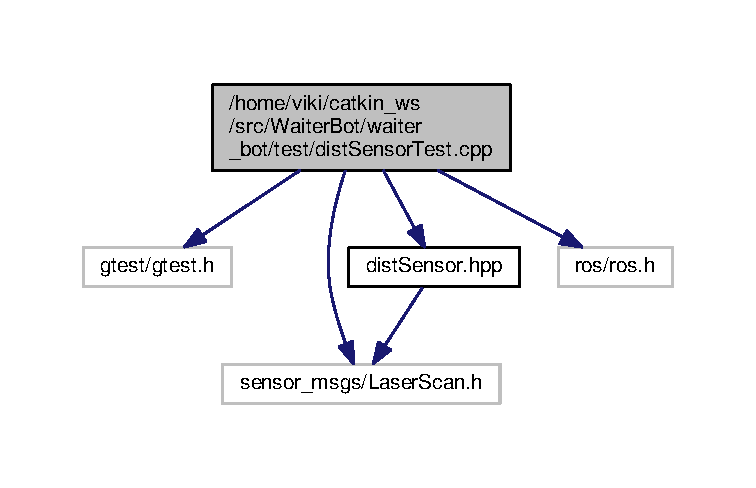
\includegraphics[width=350pt]{distSensorTest_8cpp__incl}
\end{center}
\end{figure}
\subsection*{Functions}
\begin{DoxyCompactItemize}
\item 
\hyperlink{distSensorTest_8cpp_a353927edcd78f078f772691881b849d2}{T\+E\+ST} (dist\+Sensor\+Test, constructor\+Test)
\begin{DoxyCompactList}\small\item\em test the \hyperlink{classdistSensor}{dist\+Sensor} constructor \end{DoxyCompactList}\item 
\hyperlink{distSensorTest_8cpp_ab01ffcd19d43815ddb76f948f063544a}{T\+E\+ST} (dist\+Sensor\+Test, in\+Collision\+Test)
\begin{DoxyCompactList}\small\item\em test the in\+Collison function \end{DoxyCompactList}\item 
\hyperlink{distSensorTest_8cpp_a79b5460578be96e097d06dbebdc313c6}{T\+E\+ST} (dist\+Sensor\+Test, set\+Dist\+Reading\+Call\+Back\+Test)
\begin{DoxyCompactList}\small\item\em test the set\+Dist\+Reading\+Call\+Back function \end{DoxyCompactList}\end{DoxyCompactItemize}


\subsection{Detailed Description}
This is the \char`\"{}.\+cpp\char`\"{} file for testing the \hyperlink{classdistSensor}{dist\+Sensor} class. 

\begin{DoxyAuthor}{Author}
Ruben Acevedo
\end{DoxyAuthor}
\begin{DoxyCopyright}{Copyright}
\mbox{[}2017\mbox{]} Ruben Acevedo 
\end{DoxyCopyright}


\subsection{Function Documentation}
\index{dist\+Sensor\+Test.\+cpp@{dist\+Sensor\+Test.\+cpp}!T\+E\+ST@{T\+E\+ST}}
\index{T\+E\+ST@{T\+E\+ST}!dist\+Sensor\+Test.\+cpp@{dist\+Sensor\+Test.\+cpp}}
\subsubsection[{\texorpdfstring{T\+E\+S\+T(dist\+Sensor\+Test, constructor\+Test)}{TEST(distSensorTest, constructorTest)}}]{\setlength{\rightskip}{0pt plus 5cm}T\+E\+ST (
\begin{DoxyParamCaption}
\item[{dist\+Sensor\+Test}]{, }
\item[{constructor\+Test}]{}
\end{DoxyParamCaption}
)}\hypertarget{distSensorTest_8cpp_a353927edcd78f078f772691881b849d2}{}\label{distSensorTest_8cpp_a353927edcd78f078f772691881b849d2}


test the \hyperlink{classdistSensor}{dist\+Sensor} constructor 

M\+IT License

Copyright 2017 Ruben Acevedo

Permission is hereby granted, free of charge, to any person obtaining a copy of this software and associated documentation files (the \char`\"{}\+Software\char`\"{}), to deal in the Software without restriction, including without limitation the rights to use, copy, modify, merge, publish, distribute, sublicense, and/or sell copies of the Software, and to permit persons to whom the Software is furnished to do so, subject to the following conditions\+:

The above copyright notice and this permission notice shall be included in all copies or substantial portions of the Software. T\+HE S\+O\+F\+T\+W\+A\+RE IS P\+R\+O\+V\+I\+D\+ED \char`\"{}\+A\+S I\+S\char`\"{}, W\+I\+T\+H\+O\+UT W\+A\+R\+R\+A\+N\+TY OF A\+NY K\+I\+ND, E\+X\+P\+R\+E\+SS OR I\+M\+P\+L\+I\+ED, I\+N\+C\+L\+U\+D\+I\+NG B\+UT N\+OT L\+I\+M\+I\+T\+ED TO T\+HE W\+A\+R\+R\+A\+N\+T\+I\+ES OF M\+E\+R\+C\+H\+A\+N\+T\+A\+B\+I\+L\+I\+TY, F\+I\+T\+N\+E\+SS F\+OR A P\+A\+R\+T\+I\+C\+U\+L\+AR P\+U\+R\+P\+O\+SE A\+ND N\+O\+N\+I\+N\+F\+R\+I\+N\+G\+E\+M\+E\+NT. IN NO E\+V\+E\+NT S\+H\+A\+LL T\+HE A\+U\+T\+H\+O\+RS OR C\+O\+P\+Y\+R\+I\+G\+HT H\+O\+L\+D\+E\+RS BE L\+I\+A\+B\+LE F\+OR A\+NY C\+L\+A\+IM, D\+A\+M\+A\+G\+ES OR O\+T\+H\+ER L\+I\+A\+B\+I\+L\+I\+TY, W\+H\+E\+T\+H\+ER IN AN A\+C\+T\+I\+ON OF C\+O\+N\+T\+R\+A\+CT, T\+O\+RT OR O\+T\+H\+E\+R\+W\+I\+SE, A\+R\+I\+S\+I\+NG F\+R\+OM, O\+UT OF OR IN C\+O\+N\+N\+E\+C\+T\+I\+ON W\+I\+TH T\+HE S\+O\+F\+T\+W\+A\+RE OR T\+HE U\+SE OR O\+T\+H\+ER D\+E\+A\+L\+I\+N\+GS IN T\+HE S\+O\+F\+T\+W\+A\+RE. © 2017 Git\+Hub, Inc. This tests makes sure that the constructor works It should set the dist\+Reading to be 1000000 It also test the get\+Dist\+Reading() at the same time \index{dist\+Sensor\+Test.\+cpp@{dist\+Sensor\+Test.\+cpp}!T\+E\+ST@{T\+E\+ST}}
\index{T\+E\+ST@{T\+E\+ST}!dist\+Sensor\+Test.\+cpp@{dist\+Sensor\+Test.\+cpp}}
\subsubsection[{\texorpdfstring{T\+E\+S\+T(dist\+Sensor\+Test, in\+Collision\+Test)}{TEST(distSensorTest, inCollisionTest)}}]{\setlength{\rightskip}{0pt plus 5cm}T\+E\+ST (
\begin{DoxyParamCaption}
\item[{dist\+Sensor\+Test}]{, }
\item[{in\+Collision\+Test}]{}
\end{DoxyParamCaption}
)}\hypertarget{distSensorTest_8cpp_ab01ffcd19d43815ddb76f948f063544a}{}\label{distSensorTest_8cpp_ab01ffcd19d43815ddb76f948f063544a}


test the in\+Collison function 

This tests the in\+Collision function to see if it can state whether or not the dist\+Reading idicates that something is in front of it \index{dist\+Sensor\+Test.\+cpp@{dist\+Sensor\+Test.\+cpp}!T\+E\+ST@{T\+E\+ST}}
\index{T\+E\+ST@{T\+E\+ST}!dist\+Sensor\+Test.\+cpp@{dist\+Sensor\+Test.\+cpp}}
\subsubsection[{\texorpdfstring{T\+E\+S\+T(dist\+Sensor\+Test, set\+Dist\+Reading\+Call\+Back\+Test)}{TEST(distSensorTest, setDistReadingCallBackTest)}}]{\setlength{\rightskip}{0pt plus 5cm}T\+E\+ST (
\begin{DoxyParamCaption}
\item[{dist\+Sensor\+Test}]{, }
\item[{set\+Dist\+Reading\+Call\+Back\+Test}]{}
\end{DoxyParamCaption}
)}\hypertarget{distSensorTest_8cpp_a79b5460578be96e097d06dbebdc313c6}{}\label{distSensorTest_8cpp_a79b5460578be96e097d06dbebdc313c6}


test the set\+Dist\+Reading\+Call\+Back function 

This tests the set\+Dist\+Reading\+Call\+Back function to see if can get the sensor data correctly It also retests the in\+Collision() function to make sure it marks that it is in collision 
\hypertarget{foodStubTest_8cpp}{}\section{/home/viki/catkin\+\_\+ws/src/\+Waiter\+Bot/waiter\+\_\+bot/test/food\+Stub\+Test.cpp File Reference}
\label{foodStubTest_8cpp}\index{/home/viki/catkin\+\_\+ws/src/\+Waiter\+Bot/waiter\+\_\+bot/test/food\+Stub\+Test.\+cpp@{/home/viki/catkin\+\_\+ws/src/\+Waiter\+Bot/waiter\+\_\+bot/test/food\+Stub\+Test.\+cpp}}


This is the \char`\"{}.\+cpp\char`\"{} file for testing the \hyperlink{classfoodStub}{food\+Stub} class.  


{\ttfamily \#include $<$gtest/gtest.\+h$>$}\\*
{\ttfamily \#include $<$nav\+\_\+msgs/\+Odometry.\+h$>$}\\*
{\ttfamily \#include \char`\"{}food\+Stub.\+hpp\char`\"{}}\\*
Include dependency graph for food\+Stub\+Test.\+cpp\+:
\nopagebreak
\begin{figure}[H]
\begin{center}
\leavevmode
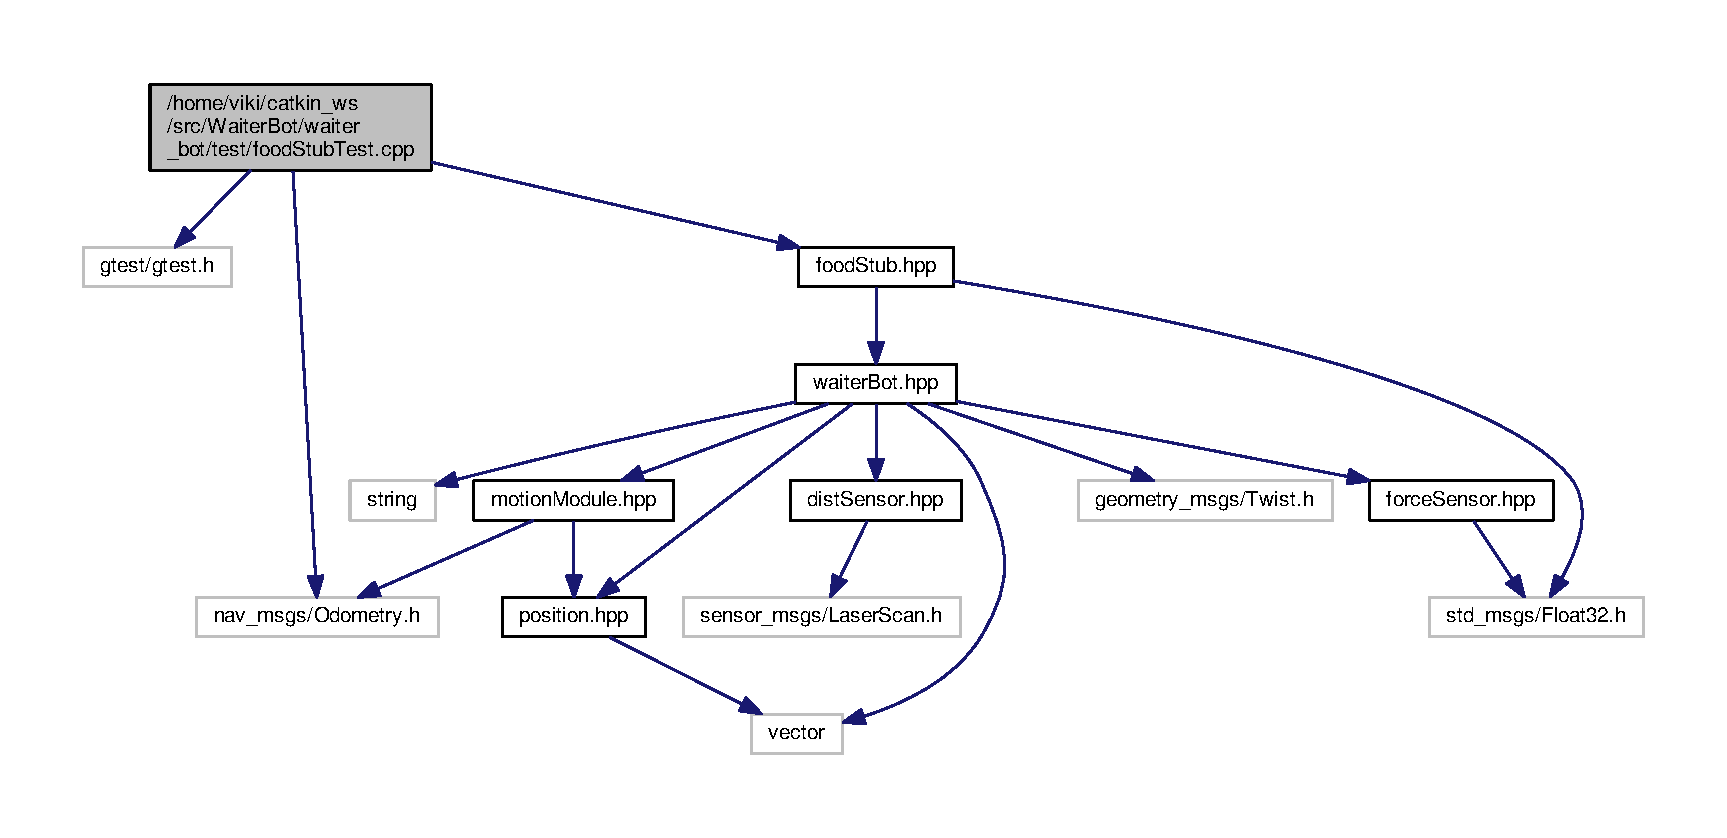
\includegraphics[width=350pt]{foodStubTest_8cpp__incl}
\end{center}
\end{figure}
\subsection*{Functions}
\begin{DoxyCompactItemize}
\item 
\hyperlink{foodStubTest_8cpp_a054c745cd6f711e32fe439e1c9e70466}{T\+E\+ST} (food\+Stub\+Test, constructor\+Test)
\begin{DoxyCompactList}\small\item\em test the food stub constructor \end{DoxyCompactList}\item 
\hyperlink{foodStubTest_8cpp_ab9c8c3ce846ef88d29c6a744a117c0a4}{T\+E\+ST} (food\+Stub\+Test, add\+Food\+Test)
\begin{DoxyCompactList}\small\item\em test the add\+Food function \end{DoxyCompactList}\item 
\hyperlink{foodStubTest_8cpp_a268a7a5f2cb05ab05eb63be40589d8c7}{T\+E\+ST} (food\+Stub\+Test, remove\+Food\+Test)
\begin{DoxyCompactList}\small\item\em test the remove\+Food function \end{DoxyCompactList}\end{DoxyCompactItemize}


\subsection{Detailed Description}
This is the \char`\"{}.\+cpp\char`\"{} file for testing the \hyperlink{classfoodStub}{food\+Stub} class. 

\begin{DoxyAuthor}{Author}
Ruben Acevedo
\end{DoxyAuthor}
\begin{DoxyCopyright}{Copyright}
\mbox{[}2017\mbox{]} Ruben Acevedo 
\end{DoxyCopyright}


\subsection{Function Documentation}
\index{food\+Stub\+Test.\+cpp@{food\+Stub\+Test.\+cpp}!T\+E\+ST@{T\+E\+ST}}
\index{T\+E\+ST@{T\+E\+ST}!food\+Stub\+Test.\+cpp@{food\+Stub\+Test.\+cpp}}
\subsubsection[{\texorpdfstring{T\+E\+S\+T(food\+Stub\+Test, constructor\+Test)}{TEST(foodStubTest, constructorTest)}}]{\setlength{\rightskip}{0pt plus 5cm}T\+E\+ST (
\begin{DoxyParamCaption}
\item[{food\+Stub\+Test}]{, }
\item[{constructor\+Test}]{}
\end{DoxyParamCaption}
)}\hypertarget{foodStubTest_8cpp_a054c745cd6f711e32fe439e1c9e70466}{}\label{foodStubTest_8cpp_a054c745cd6f711e32fe439e1c9e70466}


test the food stub constructor 

M\+IT License

Copyright 2017 Ruben Acevedo

Permission is hereby granted, free of charge, to any person obtaining a copy of this software and associated documentation files (the \char`\"{}\+Software\char`\"{}), to deal in the Software without restriction, including without limitation the rights to use, copy, modify, merge, publish, distribute, sublicense, and/or sell copies of the Software, and to permit persons to whom the Software is furnished to do so, subject to the following conditions\+:

The above copyright notice and this permission notice shall be included in all copies or substantial portions of the Software. T\+HE S\+O\+F\+T\+W\+A\+RE IS P\+R\+O\+V\+I\+D\+ED \char`\"{}\+A\+S I\+S\char`\"{}, W\+I\+T\+H\+O\+UT W\+A\+R\+R\+A\+N\+TY OF A\+NY K\+I\+ND, E\+X\+P\+R\+E\+SS OR I\+M\+P\+L\+I\+ED, I\+N\+C\+L\+U\+D\+I\+NG B\+UT N\+OT L\+I\+M\+I\+T\+ED TO T\+HE W\+A\+R\+R\+A\+N\+T\+I\+ES OF M\+E\+R\+C\+H\+A\+N\+T\+A\+B\+I\+L\+I\+TY, F\+I\+T\+N\+E\+SS F\+OR A P\+A\+R\+T\+I\+C\+U\+L\+AR P\+U\+R\+P\+O\+SE A\+ND N\+O\+N\+I\+N\+F\+R\+I\+N\+G\+E\+M\+E\+NT. IN NO E\+V\+E\+NT S\+H\+A\+LL T\+HE A\+U\+T\+H\+O\+RS OR C\+O\+P\+Y\+R\+I\+G\+HT H\+O\+L\+D\+E\+RS BE L\+I\+A\+B\+LE F\+OR A\+NY C\+L\+A\+IM, D\+A\+M\+A\+G\+ES OR O\+T\+H\+ER L\+I\+A\+B\+I\+L\+I\+TY, W\+H\+E\+T\+H\+ER IN AN A\+C\+T\+I\+ON OF C\+O\+N\+T\+R\+A\+CT, T\+O\+RT OR O\+T\+H\+E\+R\+W\+I\+SE, A\+R\+I\+S\+I\+NG F\+R\+OM, O\+UT OF OR IN C\+O\+N\+N\+E\+C\+T\+I\+ON W\+I\+TH T\+HE S\+O\+F\+T\+W\+A\+RE OR T\+HE U\+SE OR O\+T\+H\+ER D\+E\+A\+L\+I\+N\+GS IN T\+HE S\+O\+F\+T\+W\+A\+RE. © 2017 Git\+Hub, Inc. This tests makes sure that the constructor sets the food\+Weight=0 It also test the get food weight at the same time. \index{food\+Stub\+Test.\+cpp@{food\+Stub\+Test.\+cpp}!T\+E\+ST@{T\+E\+ST}}
\index{T\+E\+ST@{T\+E\+ST}!food\+Stub\+Test.\+cpp@{food\+Stub\+Test.\+cpp}}
\subsubsection[{\texorpdfstring{T\+E\+S\+T(food\+Stub\+Test, add\+Food\+Test)}{TEST(foodStubTest, addFoodTest)}}]{\setlength{\rightskip}{0pt plus 5cm}T\+E\+ST (
\begin{DoxyParamCaption}
\item[{food\+Stub\+Test}]{, }
\item[{add\+Food\+Test}]{}
\end{DoxyParamCaption}
)}\hypertarget{foodStubTest_8cpp_ab9c8c3ce846ef88d29c6a744a117c0a4}{}\label{foodStubTest_8cpp_ab9c8c3ce846ef88d29c6a744a117c0a4}


test the add\+Food function 

This tests makes sure when the add\+Food function is called it sets it to 9 Newtons \index{food\+Stub\+Test.\+cpp@{food\+Stub\+Test.\+cpp}!T\+E\+ST@{T\+E\+ST}}
\index{T\+E\+ST@{T\+E\+ST}!food\+Stub\+Test.\+cpp@{food\+Stub\+Test.\+cpp}}
\subsubsection[{\texorpdfstring{T\+E\+S\+T(food\+Stub\+Test, remove\+Food\+Test)}{TEST(foodStubTest, removeFoodTest)}}]{\setlength{\rightskip}{0pt plus 5cm}T\+E\+ST (
\begin{DoxyParamCaption}
\item[{food\+Stub\+Test}]{, }
\item[{remove\+Food\+Test}]{}
\end{DoxyParamCaption}
)}\hypertarget{foodStubTest_8cpp_a268a7a5f2cb05ab05eb63be40589d8c7}{}\label{foodStubTest_8cpp_a268a7a5f2cb05ab05eb63be40589d8c7}


test the remove\+Food function 

This tests makes sure that when remove\+Food is called the weight reduces. It also checks that the foodweight can never be negative 
\hypertarget{forceSensorTest_8cpp}{}\section{/home/viki/catkin\+\_\+ws/src/\+Waiter\+Bot/waiter\+\_\+bot/test/force\+Sensor\+Test.cpp File Reference}
\label{forceSensorTest_8cpp}\index{/home/viki/catkin\+\_\+ws/src/\+Waiter\+Bot/waiter\+\_\+bot/test/force\+Sensor\+Test.\+cpp@{/home/viki/catkin\+\_\+ws/src/\+Waiter\+Bot/waiter\+\_\+bot/test/force\+Sensor\+Test.\+cpp}}


This is the \char`\"{}.\+cpp\char`\"{} file for testing the force sensor class.  


{\ttfamily \#include $<$gtest/gtest.\+h$>$}\\*
{\ttfamily \#include $<$std\+\_\+msgs/\+Float32.\+h$>$}\\*
{\ttfamily \#include \char`\"{}force\+Sensor.\+hpp\char`\"{}}\\*
Include dependency graph for force\+Sensor\+Test.\+cpp\+:
\nopagebreak
\begin{figure}[H]
\begin{center}
\leavevmode
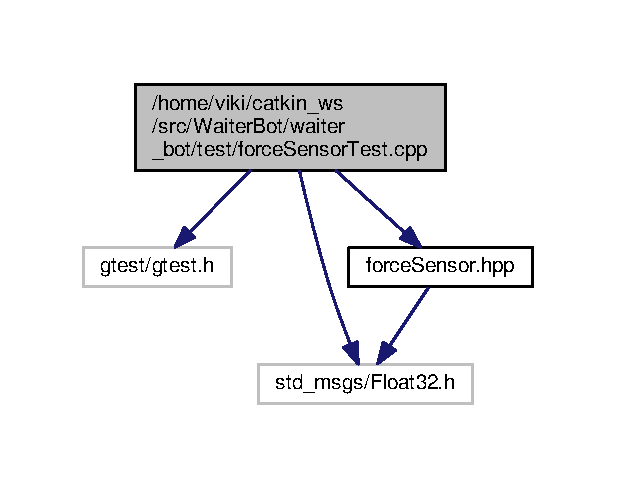
\includegraphics[width=296pt]{forceSensorTest_8cpp__incl}
\end{center}
\end{figure}
\subsection*{Functions}
\begin{DoxyCompactItemize}
\item 
\hyperlink{forceSensorTest_8cpp_a234aa624076c67e27920ce1a50022c96}{T\+E\+ST} (force\+Sensor\+Test, constructor\+Test)
\begin{DoxyCompactList}\small\item\em test the \hyperlink{classforceSensor}{force\+Sensor} constructor \end{DoxyCompactList}\item 
\hyperlink{forceSensorTest_8cpp_ac0aef936076c0a4b411872fd14361619}{T\+E\+ST} (force\+Sensor\+Test, set\+Weight\+Call\+Back\+Function\+Test)
\begin{DoxyCompactList}\small\item\em test the set weight function \end{DoxyCompactList}\end{DoxyCompactItemize}


\subsection{Detailed Description}
This is the \char`\"{}.\+cpp\char`\"{} file for testing the force sensor class. 

\begin{DoxyAuthor}{Author}
Ruben Acevedo
\end{DoxyAuthor}
\begin{DoxyCopyright}{Copyright}
\mbox{[}2017\mbox{]} Ruben Acevedo 
\end{DoxyCopyright}


\subsection{Function Documentation}
\index{force\+Sensor\+Test.\+cpp@{force\+Sensor\+Test.\+cpp}!T\+E\+ST@{T\+E\+ST}}
\index{T\+E\+ST@{T\+E\+ST}!force\+Sensor\+Test.\+cpp@{force\+Sensor\+Test.\+cpp}}
\subsubsection[{\texorpdfstring{T\+E\+S\+T(force\+Sensor\+Test, constructor\+Test)}{TEST(forceSensorTest, constructorTest)}}]{\setlength{\rightskip}{0pt plus 5cm}T\+E\+ST (
\begin{DoxyParamCaption}
\item[{force\+Sensor\+Test}]{, }
\item[{constructor\+Test}]{}
\end{DoxyParamCaption}
)}\hypertarget{forceSensorTest_8cpp_a234aa624076c67e27920ce1a50022c96}{}\label{forceSensorTest_8cpp_a234aa624076c67e27920ce1a50022c96}


test the \hyperlink{classforceSensor}{force\+Sensor} constructor 

M\+IT License

Copyright 2017 Ruben Acevedo

Permission is hereby granted, free of charge, to any person obtaining a copy of this software and associated documentation files (the \char`\"{}\+Software\char`\"{}), to deal in the Software without restriction, including without limitation the rights to use, copy, modify, merge, publish, distribute, sublicense, and/or sell copies of the Software, and to permit persons to whom the Software is furnished to do so, subject to the following conditions\+:

The above copyright notice and this permission notice shall be included in all copies or substantial portions of the Software. T\+HE S\+O\+F\+T\+W\+A\+RE IS P\+R\+O\+V\+I\+D\+ED \char`\"{}\+A\+S I\+S\char`\"{}, W\+I\+T\+H\+O\+UT W\+A\+R\+R\+A\+N\+TY OF A\+NY K\+I\+ND, E\+X\+P\+R\+E\+SS OR I\+M\+P\+L\+I\+ED, I\+N\+C\+L\+U\+D\+I\+NG B\+UT N\+OT L\+I\+M\+I\+T\+ED TO T\+HE W\+A\+R\+R\+A\+N\+T\+I\+ES OF M\+E\+R\+C\+H\+A\+N\+T\+A\+B\+I\+L\+I\+TY, F\+I\+T\+N\+E\+SS F\+OR A P\+A\+R\+T\+I\+C\+U\+L\+AR P\+U\+R\+P\+O\+SE A\+ND N\+O\+N\+I\+N\+F\+R\+I\+N\+G\+E\+M\+E\+NT. IN NO E\+V\+E\+NT S\+H\+A\+LL T\+HE A\+U\+T\+H\+O\+RS OR C\+O\+P\+Y\+R\+I\+G\+HT H\+O\+L\+D\+E\+RS BE L\+I\+A\+B\+LE F\+OR A\+NY C\+L\+A\+IM, D\+A\+M\+A\+G\+ES OR O\+T\+H\+ER L\+I\+A\+B\+I\+L\+I\+TY, W\+H\+E\+T\+H\+ER IN AN A\+C\+T\+I\+ON OF C\+O\+N\+T\+R\+A\+CT, T\+O\+RT OR O\+T\+H\+E\+R\+W\+I\+SE, A\+R\+I\+S\+I\+NG F\+R\+OM, O\+UT OF OR IN C\+O\+N\+N\+E\+C\+T\+I\+ON W\+I\+TH T\+HE S\+O\+F\+T\+W\+A\+RE OR T\+HE U\+SE OR O\+T\+H\+ER D\+E\+A\+L\+I\+N\+GS IN T\+HE S\+O\+F\+T\+W\+A\+RE. © 2017 Git\+Hub, Inc. This tests makes sure that the constructor sets the Weight=-\/1 It also test the get food weight at the same time. \index{force\+Sensor\+Test.\+cpp@{force\+Sensor\+Test.\+cpp}!T\+E\+ST@{T\+E\+ST}}
\index{T\+E\+ST@{T\+E\+ST}!force\+Sensor\+Test.\+cpp@{force\+Sensor\+Test.\+cpp}}
\subsubsection[{\texorpdfstring{T\+E\+S\+T(force\+Sensor\+Test, set\+Weight\+Call\+Back\+Function\+Test)}{TEST(forceSensorTest, setWeightCallBackFunctionTest)}}]{\setlength{\rightskip}{0pt plus 5cm}T\+E\+ST (
\begin{DoxyParamCaption}
\item[{force\+Sensor\+Test}]{, }
\item[{set\+Weight\+Call\+Back\+Function\+Test}]{}
\end{DoxyParamCaption}
)}\hypertarget{forceSensorTest_8cpp_ac0aef936076c0a4b411872fd14361619}{}\label{forceSensorTest_8cpp_ac0aef936076c0a4b411872fd14361619}


test the set weight function 

This tests makes sure the function sets the weight given a Float32 message 
\hypertarget{mainTest_8cpp}{}\section{/home/viki/catkin\+\_\+ws/src/\+Waiter\+Bot/waiter\+\_\+bot/test/main\+Test.cpp File Reference}
\label{mainTest_8cpp}\index{/home/viki/catkin\+\_\+ws/src/\+Waiter\+Bot/waiter\+\_\+bot/test/main\+Test.\+cpp@{/home/viki/catkin\+\_\+ws/src/\+Waiter\+Bot/waiter\+\_\+bot/test/main\+Test.\+cpp}}


This is the \char`\"{}.\+cpp\char`\"{} file for the int \hyperlink{mainTest_8cpp_a3c04138a5bfe5d72780bb7e82a18e627}{main()}  


{\ttfamily \#include $<$gtest/gtest.\+h$>$}\\*
{\ttfamily \#include $<$ros/ros.\+h$>$}\\*
Include dependency graph for main\+Test.\+cpp\+:
\nopagebreak
\begin{figure}[H]
\begin{center}
\leavevmode
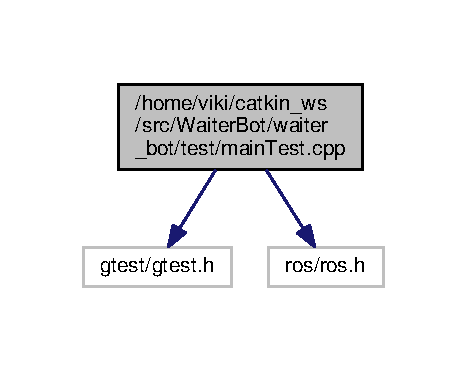
\includegraphics[width=224pt]{mainTest_8cpp__incl}
\end{center}
\end{figure}
\subsection*{Functions}
\begin{DoxyCompactItemize}
\item 
int \hyperlink{mainTest_8cpp_a3c04138a5bfe5d72780bb7e82a18e627}{main} (int argc, char $\ast$$\ast$argv)
\begin{DoxyCompactList}\small\item\em int \hyperlink{mainTest_8cpp_a3c04138a5bfe5d72780bb7e82a18e627}{main()} for tests \end{DoxyCompactList}\end{DoxyCompactItemize}


\subsection{Detailed Description}
This is the \char`\"{}.\+cpp\char`\"{} file for the int \hyperlink{mainTest_8cpp_a3c04138a5bfe5d72780bb7e82a18e627}{main()} 

\begin{DoxyAuthor}{Author}
Ruben Acevedo
\end{DoxyAuthor}
\begin{DoxyCopyright}{Copyright}
\mbox{[}2017\mbox{]} Ruben Acevedo 
\end{DoxyCopyright}


\subsection{Function Documentation}
\index{main\+Test.\+cpp@{main\+Test.\+cpp}!main@{main}}
\index{main@{main}!main\+Test.\+cpp@{main\+Test.\+cpp}}
\subsubsection[{\texorpdfstring{main(int argc, char $\ast$$\ast$argv)}{main(int argc, char **argv)}}]{\setlength{\rightskip}{0pt plus 5cm}int main (
\begin{DoxyParamCaption}
\item[{int}]{argc, }
\item[{char $\ast$$\ast$}]{argv}
\end{DoxyParamCaption}
)}\hypertarget{mainTest_8cpp_a3c04138a5bfe5d72780bb7e82a18e627}{}\label{mainTest_8cpp_a3c04138a5bfe5d72780bb7e82a18e627}


int \hyperlink{mainTest_8cpp_a3c04138a5bfe5d72780bb7e82a18e627}{main()} for tests 

M\+IT License

Copyright 2017 Ruben Acevedo

Permission is hereby granted, free of charge, to any person obtaining a copy of this software and associated documentation files (the \char`\"{}\+Software\char`\"{}), to deal in the Software without restriction, including without limitation the rights to use, copy, modify, merge, publish, distribute, sublicense, and/or sell copies of the Software, and to permit persons to whom the Software is furnished to do so, subject to the following conditions\+:

The above copyright notice and this permission notice shall be included in all copies or substantial portions of the Software. T\+HE S\+O\+F\+T\+W\+A\+RE IS P\+R\+O\+V\+I\+D\+ED \char`\"{}\+A\+S I\+S\char`\"{}, W\+I\+T\+H\+O\+UT W\+A\+R\+R\+A\+N\+TY OF A\+NY K\+I\+ND, E\+X\+P\+R\+E\+SS OR I\+M\+P\+L\+I\+ED, I\+N\+C\+L\+U\+D\+I\+NG B\+UT N\+OT L\+I\+M\+I\+T\+ED TO T\+HE W\+A\+R\+R\+A\+N\+T\+I\+ES OF M\+E\+R\+C\+H\+A\+N\+T\+A\+B\+I\+L\+I\+TY, F\+I\+T\+N\+E\+SS F\+OR A P\+A\+R\+T\+I\+C\+U\+L\+AR P\+U\+R\+P\+O\+SE A\+ND N\+O\+N\+I\+N\+F\+R\+I\+N\+G\+E\+M\+E\+NT. IN NO E\+V\+E\+NT S\+H\+A\+LL T\+HE A\+U\+T\+H\+O\+RS OR C\+O\+P\+Y\+R\+I\+G\+HT H\+O\+L\+D\+E\+RS BE L\+I\+A\+B\+LE F\+OR A\+NY C\+L\+A\+IM, D\+A\+M\+A\+G\+ES OR O\+T\+H\+ER L\+I\+A\+B\+I\+L\+I\+TY, W\+H\+E\+T\+H\+ER IN AN A\+C\+T\+I\+ON OF C\+O\+N\+T\+R\+A\+CT, T\+O\+RT OR O\+T\+H\+E\+R\+W\+I\+SE, A\+R\+I\+S\+I\+NG F\+R\+OM, O\+UT OF OR IN C\+O\+N\+N\+E\+C\+T\+I\+ON W\+I\+TH T\+HE S\+O\+F\+T\+W\+A\+RE OR T\+HE U\+SE OR O\+T\+H\+ER D\+E\+A\+L\+I\+N\+GS IN T\+HE S\+O\+F\+T\+W\+A\+RE. © 2017 Git\+Hub, Inc. This runs all the test in the test folder 
\hypertarget{motionModuleTest_8cpp}{}\section{/home/viki/catkin\+\_\+ws/src/\+Waiter\+Bot/waiter\+\_\+bot/test/motion\+Module\+Test.cpp File Reference}
\label{motionModuleTest_8cpp}\index{/home/viki/catkin\+\_\+ws/src/\+Waiter\+Bot/waiter\+\_\+bot/test/motion\+Module\+Test.\+cpp@{/home/viki/catkin\+\_\+ws/src/\+Waiter\+Bot/waiter\+\_\+bot/test/motion\+Module\+Test.\+cpp}}


This is the \char`\"{}.\+cpp\char`\"{} file for testing the \hyperlink{classmotionModule}{motion\+Module} class.  


{\ttfamily \#include $<$gtest/gtest.\+h$>$}\\*
{\ttfamily \#include $<$nav\+\_\+msgs/\+Odometry.\+h$>$}\\*
{\ttfamily \#include \char`\"{}motion\+Module.\+hpp\char`\"{}}\\*
{\ttfamily \#include \char`\"{}position.\+hpp\char`\"{}}\\*
Include dependency graph for motion\+Module\+Test.\+cpp\+:
\nopagebreak
\begin{figure}[H]
\begin{center}
\leavevmode
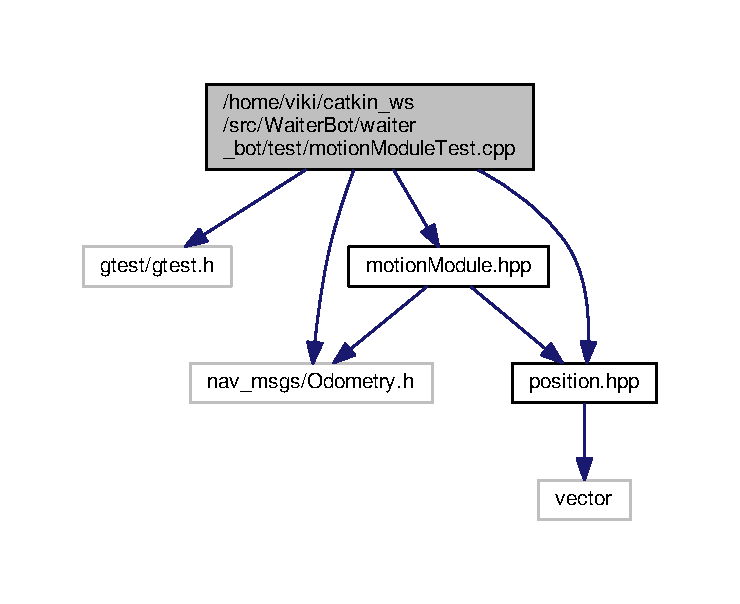
\includegraphics[width=350pt]{motionModuleTest_8cpp__incl}
\end{center}
\end{figure}
\subsection*{Functions}
\begin{DoxyCompactItemize}
\item 
\hyperlink{motionModuleTest_8cpp_a947074b8a1bbcf6db6ad6bced96e1f8e}{T\+E\+ST} (motion\+Module\+Test, get\+Current\+Loc\+Test)
\begin{DoxyCompactList}\small\item\em test the get\+Current\+Loc function \end{DoxyCompactList}\item 
\hyperlink{motionModuleTest_8cpp_aa60e14fdeb1891a8921237901fa402ec}{T\+E\+ST} (motion\+Module\+Test, in\+Region\+Test)
\begin{DoxyCompactList}\small\item\em test the in\+Region function \end{DoxyCompactList}\item 
\hyperlink{motionModuleTest_8cpp_afd8b2bdf60fd0ecb6b38dd95c2a8767a}{T\+E\+ST} (motion\+Module\+Test, set\+Current\+Location\+Call\+Back\+Test)
\begin{DoxyCompactList}\small\item\em test the set current location function \end{DoxyCompactList}\item 
\hyperlink{motionModuleTest_8cpp_a9409f9dae0de728a5eac6916c158be25}{T\+E\+ST} (motion\+Module\+Test, set\+Theta\+Value\+For\+Tests\+Test)
\begin{DoxyCompactList}\small\item\em test the set current location function \end{DoxyCompactList}\end{DoxyCompactItemize}


\subsection{Detailed Description}
This is the \char`\"{}.\+cpp\char`\"{} file for testing the \hyperlink{classmotionModule}{motion\+Module} class. 

\begin{DoxyAuthor}{Author}
Ruben Acevedo
\end{DoxyAuthor}
\begin{DoxyCopyright}{Copyright}
\mbox{[}2017\mbox{]} Ruben Acevedo 
\end{DoxyCopyright}


\subsection{Function Documentation}
\index{motion\+Module\+Test.\+cpp@{motion\+Module\+Test.\+cpp}!T\+E\+ST@{T\+E\+ST}}
\index{T\+E\+ST@{T\+E\+ST}!motion\+Module\+Test.\+cpp@{motion\+Module\+Test.\+cpp}}
\subsubsection[{\texorpdfstring{T\+E\+S\+T(motion\+Module\+Test, get\+Current\+Loc\+Test)}{TEST(motionModuleTest, getCurrentLocTest)}}]{\setlength{\rightskip}{0pt plus 5cm}T\+E\+ST (
\begin{DoxyParamCaption}
\item[{motion\+Module\+Test}]{, }
\item[{get\+Current\+Loc\+Test}]{}
\end{DoxyParamCaption}
)}\hypertarget{motionModuleTest_8cpp_a947074b8a1bbcf6db6ad6bced96e1f8e}{}\label{motionModuleTest_8cpp_a947074b8a1bbcf6db6ad6bced96e1f8e}


test the get\+Current\+Loc function 

M\+IT License

Copyright 2017 Ruben Acevedo

Permission is hereby granted, free of charge, to any person obtaining a copy of this software and associated documentation files (the \char`\"{}\+Software\char`\"{}), to deal in the Software without restriction, including without limitation the rights to use, copy, modify, merge, publish, distribute, sublicense, and/or sell copies of the Software, and to permit persons to whom the Software is furnished to do so, subject to the following conditions\+:

The above copyright notice and this permission notice shall be included in all copies or substantial portions of the Software. T\+HE S\+O\+F\+T\+W\+A\+RE IS P\+R\+O\+V\+I\+D\+ED \char`\"{}\+A\+S I\+S\char`\"{}, W\+I\+T\+H\+O\+UT W\+A\+R\+R\+A\+N\+TY OF A\+NY K\+I\+ND, E\+X\+P\+R\+E\+SS OR I\+M\+P\+L\+I\+ED, I\+N\+C\+L\+U\+D\+I\+NG B\+UT N\+OT L\+I\+M\+I\+T\+ED TO T\+HE W\+A\+R\+R\+A\+N\+T\+I\+ES OF M\+E\+R\+C\+H\+A\+N\+T\+A\+B\+I\+L\+I\+TY, F\+I\+T\+N\+E\+SS F\+OR A P\+A\+R\+T\+I\+C\+U\+L\+AR P\+U\+R\+P\+O\+SE A\+ND N\+O\+N\+I\+N\+F\+R\+I\+N\+G\+E\+M\+E\+NT. IN NO E\+V\+E\+NT S\+H\+A\+LL T\+HE A\+U\+T\+H\+O\+RS OR C\+O\+P\+Y\+R\+I\+G\+HT H\+O\+L\+D\+E\+RS BE L\+I\+A\+B\+LE F\+OR A\+NY C\+L\+A\+IM, D\+A\+M\+A\+G\+ES OR O\+T\+H\+ER L\+I\+A\+B\+I\+L\+I\+TY, W\+H\+E\+T\+H\+ER IN AN A\+C\+T\+I\+ON OF C\+O\+N\+T\+R\+A\+CT, T\+O\+RT OR O\+T\+H\+E\+R\+W\+I\+SE, A\+R\+I\+S\+I\+NG F\+R\+OM, O\+UT OF OR IN C\+O\+N\+N\+E\+C\+T\+I\+ON W\+I\+TH T\+HE S\+O\+F\+T\+W\+A\+RE OR T\+HE U\+SE OR O\+T\+H\+ER D\+E\+A\+L\+I\+N\+GS IN T\+HE S\+O\+F\+T\+W\+A\+RE. © 2017 Git\+Hub, Inc. This tests makes sure that it returns the current location \index{motion\+Module\+Test.\+cpp@{motion\+Module\+Test.\+cpp}!T\+E\+ST@{T\+E\+ST}}
\index{T\+E\+ST@{T\+E\+ST}!motion\+Module\+Test.\+cpp@{motion\+Module\+Test.\+cpp}}
\subsubsection[{\texorpdfstring{T\+E\+S\+T(motion\+Module\+Test, in\+Region\+Test)}{TEST(motionModuleTest, inRegionTest)}}]{\setlength{\rightskip}{0pt plus 5cm}T\+E\+ST (
\begin{DoxyParamCaption}
\item[{motion\+Module\+Test}]{, }
\item[{in\+Region\+Test}]{}
\end{DoxyParamCaption}
)}\hypertarget{motionModuleTest_8cpp_aa60e14fdeb1891a8921237901fa402ec}{}\label{motionModuleTest_8cpp_aa60e14fdeb1891a8921237901fa402ec}


test the in\+Region function 

This tests makes test the in\+Region function it should output true if current location is with in a 0.\+125 m distance from the input position \index{motion\+Module\+Test.\+cpp@{motion\+Module\+Test.\+cpp}!T\+E\+ST@{T\+E\+ST}}
\index{T\+E\+ST@{T\+E\+ST}!motion\+Module\+Test.\+cpp@{motion\+Module\+Test.\+cpp}}
\subsubsection[{\texorpdfstring{T\+E\+S\+T(motion\+Module\+Test, set\+Current\+Location\+Call\+Back\+Test)}{TEST(motionModuleTest, setCurrentLocationCallBackTest)}}]{\setlength{\rightskip}{0pt plus 5cm}T\+E\+ST (
\begin{DoxyParamCaption}
\item[{motion\+Module\+Test}]{, }
\item[{set\+Current\+Location\+Call\+Back\+Test}]{}
\end{DoxyParamCaption}
)}\hypertarget{motionModuleTest_8cpp_afd8b2bdf60fd0ecb6b38dd95c2a8767a}{}\label{motionModuleTest_8cpp_afd8b2bdf60fd0ecb6b38dd95c2a8767a}


test the set current location function 

This tests the set\+Current\+Location\+Call\+Back it should set current\+Loc to what ever the nav\+\_\+msgs\+::\+Odometry message is with in a 0.\+125 m distance from the input position \index{motion\+Module\+Test.\+cpp@{motion\+Module\+Test.\+cpp}!T\+E\+ST@{T\+E\+ST}}
\index{T\+E\+ST@{T\+E\+ST}!motion\+Module\+Test.\+cpp@{motion\+Module\+Test.\+cpp}}
\subsubsection[{\texorpdfstring{T\+E\+S\+T(motion\+Module\+Test, set\+Theta\+Value\+For\+Tests\+Test)}{TEST(motionModuleTest, setThetaValueForTestsTest)}}]{\setlength{\rightskip}{0pt plus 5cm}T\+E\+ST (
\begin{DoxyParamCaption}
\item[{motion\+Module\+Test}]{, }
\item[{set\+Theta\+Value\+For\+Tests\+Test}]{}
\end{DoxyParamCaption}
)}\hypertarget{motionModuleTest_8cpp_a9409f9dae0de728a5eac6916c158be25}{}\label{motionModuleTest_8cpp_a9409f9dae0de728a5eac6916c158be25}


test the set current location function 

This tests the set\+Current\+Location\+Call\+Back it should set current\+Loc to what ever the nav\+\_\+msgs\+::\+Odometry message is with in a 0.\+125 m distance from the input position 
\hypertarget{nodeInteractionsTest_8cpp}{}\section{/home/viki/catkin\+\_\+ws/src/\+Waiter\+Bot/waiter\+\_\+bot/test/node\+Interactions\+Test.cpp File Reference}
\label{nodeInteractionsTest_8cpp}\index{/home/viki/catkin\+\_\+ws/src/\+Waiter\+Bot/waiter\+\_\+bot/test/node\+Interactions\+Test.\+cpp@{/home/viki/catkin\+\_\+ws/src/\+Waiter\+Bot/waiter\+\_\+bot/test/node\+Interactions\+Test.\+cpp}}


This is the \char`\"{}.\+cpp\char`\"{} file for testing the node interations.  


{\ttfamily \#include $<$gtest/gtest.\+h$>$}\\*
{\ttfamily \#include $<$geometry\+\_\+msgs/\+Twist.\+h$>$}\\*
{\ttfamily \#include $<$std\+\_\+msgs/\+Float32.\+h$>$}\\*
{\ttfamily \#include \char`\"{}ros/ros.\+h\char`\"{}}\\*
Include dependency graph for node\+Interactions\+Test.\+cpp\+:
\nopagebreak
\begin{figure}[H]
\begin{center}
\leavevmode
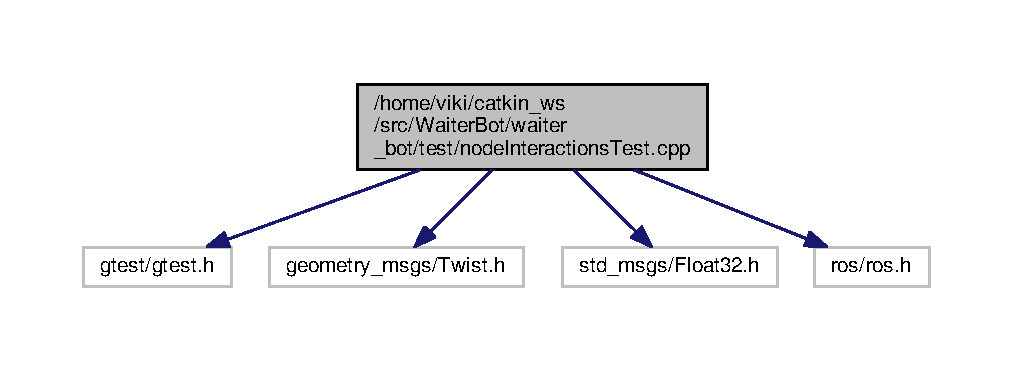
\includegraphics[width=350pt]{nodeInteractionsTest_8cpp__incl}
\end{center}
\end{figure}
\subsection*{Functions}
\begin{DoxyCompactItemize}
\item 
void {\bfseries vel\+Call\+Back} (const geometry\+\_\+msgs\+::\+Twist \&vel)\hypertarget{nodeInteractionsTest_8cpp_af9a1162f222b8b602ddc21b31aef0cb9}{}\label{nodeInteractionsTest_8cpp_af9a1162f222b8b602ddc21b31aef0cb9}

\item 
void {\bfseries force\+Call\+Back} (const std\+\_\+msgs\+::\+Float32 \&f\+\_\+msg)\hypertarget{nodeInteractionsTest_8cpp_a92094d561888a0a18f78a63b4ea3248f}{}\label{nodeInteractionsTest_8cpp_a92094d561888a0a18f78a63b4ea3248f}

\item 
\hyperlink{nodeInteractionsTest_8cpp_a871117ce018faf9047061b943d7fed57}{T\+E\+ST} (node\+Interactions\+Test, waiter\+Bot\+\_\+node\+Test)
\begin{DoxyCompactList}\small\item\em test the waiter\+Bot\+\_\+node \end{DoxyCompactList}\item 
\hyperlink{nodeInteractionsTest_8cpp_a50ef1f939ceba54b3ae4e0c8f4f2696a}{T\+E\+ST} (node\+Interactions\+Test, food\+Stub\+\_\+node\+Test)
\begin{DoxyCompactList}\small\item\em test the food\+Stub\+\_\+node \end{DoxyCompactList}\end{DoxyCompactItemize}
\subsection*{Variables}
\begin{DoxyCompactItemize}
\item 
float \hyperlink{nodeInteractionsTest_8cpp_ad0da36b2558901e21e7a30f6c227a45e}{x}
\item 
float {\bfseries t}\hypertarget{nodeInteractionsTest_8cpp_afea36502e9d227ff62c5fb2719a246f2}{}\label{nodeInteractionsTest_8cpp_afea36502e9d227ff62c5fb2719a246f2}

\item 
bool {\bfseries velB}\hypertarget{nodeInteractionsTest_8cpp_a92c36b07bc31e8b04d8670c9a389d04f}{}\label{nodeInteractionsTest_8cpp_a92c36b07bc31e8b04d8670c9a389d04f}

\item 
float {\bfseries w}\hypertarget{nodeInteractionsTest_8cpp_a56eca241e2896b9f57a79589e76fd24b}{}\label{nodeInteractionsTest_8cpp_a56eca241e2896b9f57a79589e76fd24b}

\item 
bool {\bfseries forceB}\hypertarget{nodeInteractionsTest_8cpp_a06b51cfbf437b516a1289dab2b0eade3}{}\label{nodeInteractionsTest_8cpp_a06b51cfbf437b516a1289dab2b0eade3}

\end{DoxyCompactItemize}


\subsection{Detailed Description}
This is the \char`\"{}.\+cpp\char`\"{} file for testing the node interations. 

\begin{DoxyAuthor}{Author}
Ruben Acevedo
\end{DoxyAuthor}
\begin{DoxyCopyright}{Copyright}
\mbox{[}2017\mbox{]} Ruben Acevedo 
\end{DoxyCopyright}


\subsection{Function Documentation}
\index{node\+Interactions\+Test.\+cpp@{node\+Interactions\+Test.\+cpp}!T\+E\+ST@{T\+E\+ST}}
\index{T\+E\+ST@{T\+E\+ST}!node\+Interactions\+Test.\+cpp@{node\+Interactions\+Test.\+cpp}}
\subsubsection[{\texorpdfstring{T\+E\+S\+T(node\+Interactions\+Test, waiter\+Bot\+\_\+node\+Test)}{TEST(nodeInteractionsTest, waiterBot_nodeTest)}}]{\setlength{\rightskip}{0pt plus 5cm}T\+E\+ST (
\begin{DoxyParamCaption}
\item[{node\+Interactions\+Test}]{, }
\item[{waiter\+Bot\+\_\+node\+Test}]{}
\end{DoxyParamCaption}
)}\hypertarget{nodeInteractionsTest_8cpp_a871117ce018faf9047061b943d7fed57}{}\label{nodeInteractionsTest_8cpp_a871117ce018faf9047061b943d7fed57}


test the waiter\+Bot\+\_\+node 

This tests the waiter\+Bot\+\_\+node Given that the \hyperlink{classdistSensor}{dist\+Sensor} should be recieving a collision statement. The \hyperlink{classwaiterBot}{waiter\+Bot} should be publishing linear.\+x = angular.\+z = 0 \index{node\+Interactions\+Test.\+cpp@{node\+Interactions\+Test.\+cpp}!T\+E\+ST@{T\+E\+ST}}
\index{T\+E\+ST@{T\+E\+ST}!node\+Interactions\+Test.\+cpp@{node\+Interactions\+Test.\+cpp}}
\subsubsection[{\texorpdfstring{T\+E\+S\+T(node\+Interactions\+Test, food\+Stub\+\_\+node\+Test)}{TEST(nodeInteractionsTest, foodStub_nodeTest)}}]{\setlength{\rightskip}{0pt plus 5cm}T\+E\+ST (
\begin{DoxyParamCaption}
\item[{node\+Interactions\+Test}]{, }
\item[{food\+Stub\+\_\+node\+Test}]{}
\end{DoxyParamCaption}
)}\hypertarget{nodeInteractionsTest_8cpp_a50ef1f939ceba54b3ae4e0c8f4f2696a}{}\label{nodeInteractionsTest_8cpp_a50ef1f939ceba54b3ae4e0c8f4f2696a}


test the food\+Stub\+\_\+node 

This tests the food\+Stub\+\_\+node Given that the robot should be at location (0,2) the food stub should be publishing data = 6.\+033 

\subsection{Variable Documentation}
\index{node\+Interactions\+Test.\+cpp@{node\+Interactions\+Test.\+cpp}!x@{x}}
\index{x@{x}!node\+Interactions\+Test.\+cpp@{node\+Interactions\+Test.\+cpp}}
\subsubsection[{\texorpdfstring{x}{x}}]{\setlength{\rightskip}{0pt plus 5cm}float x}\hypertarget{nodeInteractionsTest_8cpp_ad0da36b2558901e21e7a30f6c227a45e}{}\label{nodeInteractionsTest_8cpp_ad0da36b2558901e21e7a30f6c227a45e}
M\+IT License

Copyright 2017 Ruben Acevedo

Permission is hereby granted, free of charge, to any person obtaining a copy of this software and associated documentation files (the \char`\"{}\+Software\char`\"{}), to deal in the Software without restriction, including without limitation the rights to use, copy, modify, merge, publish, distribute, sublicense, and/or sell copies of the Software, and to permit persons to whom the Software is furnished to do so, subject to the following conditions\+:

The above copyright notice and this permission notice shall be included in all copies or substantial portions of the Software. T\+HE S\+O\+F\+T\+W\+A\+RE IS P\+R\+O\+V\+I\+D\+ED \char`\"{}\+A\+S I\+S\char`\"{}, W\+I\+T\+H\+O\+UT W\+A\+R\+R\+A\+N\+TY OF A\+NY K\+I\+ND, E\+X\+P\+R\+E\+SS OR I\+M\+P\+L\+I\+ED, I\+N\+C\+L\+U\+D\+I\+NG B\+UT N\+OT L\+I\+M\+I\+T\+ED TO T\+HE W\+A\+R\+R\+A\+N\+T\+I\+ES OF M\+E\+R\+C\+H\+A\+N\+T\+A\+B\+I\+L\+I\+TY, F\+I\+T\+N\+E\+SS F\+OR A P\+A\+R\+T\+I\+C\+U\+L\+AR P\+U\+R\+P\+O\+SE A\+ND N\+O\+N\+I\+N\+F\+R\+I\+N\+G\+E\+M\+E\+NT. IN NO E\+V\+E\+NT S\+H\+A\+LL T\+HE A\+U\+T\+H\+O\+RS OR C\+O\+P\+Y\+R\+I\+G\+HT H\+O\+L\+D\+E\+RS BE L\+I\+A\+B\+LE F\+OR A\+NY C\+L\+A\+IM, D\+A\+M\+A\+G\+ES OR O\+T\+H\+ER L\+I\+A\+B\+I\+L\+I\+TY, W\+H\+E\+T\+H\+ER IN AN A\+C\+T\+I\+ON OF C\+O\+N\+T\+R\+A\+CT, T\+O\+RT OR O\+T\+H\+E\+R\+W\+I\+SE, A\+R\+I\+S\+I\+NG F\+R\+OM, O\+UT OF OR IN C\+O\+N\+N\+E\+C\+T\+I\+ON W\+I\+TH T\+HE S\+O\+F\+T\+W\+A\+RE OR T\+HE U\+SE OR O\+T\+H\+ER D\+E\+A\+L\+I\+N\+GS IN T\+HE S\+O\+F\+T\+W\+A\+RE. © 2017 Git\+Hub, Inc. 
\hypertarget{positionTest_8cpp}{}\section{/home/viki/catkin\+\_\+ws/src/\+Waiter\+Bot/waiter\+\_\+bot/test/position\+Test.cpp File Reference}
\label{positionTest_8cpp}\index{/home/viki/catkin\+\_\+ws/src/\+Waiter\+Bot/waiter\+\_\+bot/test/position\+Test.\+cpp@{/home/viki/catkin\+\_\+ws/src/\+Waiter\+Bot/waiter\+\_\+bot/test/position\+Test.\+cpp}}


This is the \char`\"{}.\+cpp\char`\"{} file for testing the position class.  


{\ttfamily \#include $<$gtest/gtest.\+h$>$}\\*
{\ttfamily \#include $<$vector$>$}\\*
{\ttfamily \#include \char`\"{}position.\+hpp\char`\"{}}\\*
Include dependency graph for position\+Test.\+cpp\+:
\nopagebreak
\begin{figure}[H]
\begin{center}
\leavevmode
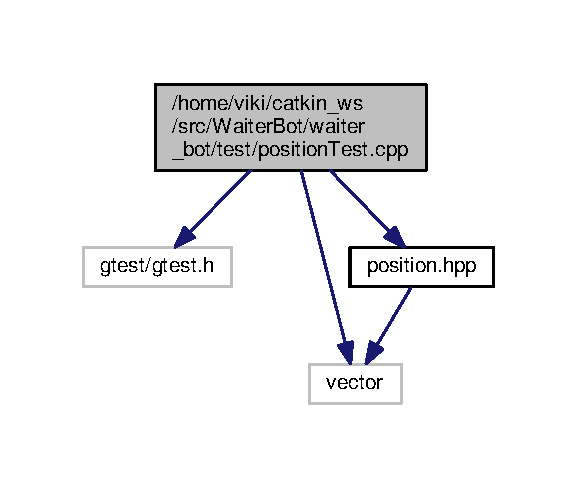
\includegraphics[width=277pt]{positionTest_8cpp__incl}
\end{center}
\end{figure}
\subsection*{Functions}
\begin{DoxyCompactItemize}
\item 
\hyperlink{positionTest_8cpp_abcb69c48c1d68181560bfe6a73e06aea}{T\+E\+ST} (position\+Test, constructor\+Test)
\begin{DoxyCompactList}\small\item\em test the position constructor \end{DoxyCompactList}\item 
\hyperlink{positionTest_8cpp_a79a9a70083eb7a5830ef50f848b43f8c}{T\+E\+ST} (position\+Test, set\+Position\+Test)
\begin{DoxyCompactList}\small\item\em test the set\+Position function \end{DoxyCompactList}\end{DoxyCompactItemize}


\subsection{Detailed Description}
This is the \char`\"{}.\+cpp\char`\"{} file for testing the position class. 

\begin{DoxyAuthor}{Author}
Ruben Acevedo
\end{DoxyAuthor}
\begin{DoxyCopyright}{Copyright}
\mbox{[}2017\mbox{]} Ruben Acevedo 
\end{DoxyCopyright}


\subsection{Function Documentation}
\index{position\+Test.\+cpp@{position\+Test.\+cpp}!T\+E\+ST@{T\+E\+ST}}
\index{T\+E\+ST@{T\+E\+ST}!position\+Test.\+cpp@{position\+Test.\+cpp}}
\subsubsection[{\texorpdfstring{T\+E\+S\+T(position\+Test, constructor\+Test)}{TEST(positionTest, constructorTest)}}]{\setlength{\rightskip}{0pt plus 5cm}T\+E\+ST (
\begin{DoxyParamCaption}
\item[{position\+Test}]{, }
\item[{constructor\+Test}]{}
\end{DoxyParamCaption}
)}\hypertarget{positionTest_8cpp_abcb69c48c1d68181560bfe6a73e06aea}{}\label{positionTest_8cpp_abcb69c48c1d68181560bfe6a73e06aea}


test the position constructor 

M\+IT License

Copyright 2017 Ruben Acevedo

Permission is hereby granted, free of charge, to any person obtaining a copy of this software and associated documentation files (the \char`\"{}\+Software\char`\"{}), to deal in the Software without restriction, including without limitation the rights to use, copy, modify, merge, publish, distribute, sublicense, and/or sell copies of the Software, and to permit persons to whom the Software is furnished to do so, subject to the following conditions\+:

The above copyright notice and this permission notice shall be included in all copies or substantial portions of the Software. T\+HE S\+O\+F\+T\+W\+A\+RE IS P\+R\+O\+V\+I\+D\+ED \char`\"{}\+A\+S I\+S\char`\"{}, W\+I\+T\+H\+O\+UT W\+A\+R\+R\+A\+N\+TY OF A\+NY K\+I\+ND, E\+X\+P\+R\+E\+SS OR I\+M\+P\+L\+I\+ED, I\+N\+C\+L\+U\+D\+I\+NG B\+UT N\+OT L\+I\+M\+I\+T\+ED TO T\+HE W\+A\+R\+R\+A\+N\+T\+I\+ES OF M\+E\+R\+C\+H\+A\+N\+T\+A\+B\+I\+L\+I\+TY, F\+I\+T\+N\+E\+SS F\+OR A P\+A\+R\+T\+I\+C\+U\+L\+AR P\+U\+R\+P\+O\+SE A\+ND N\+O\+N\+I\+N\+F\+R\+I\+N\+G\+E\+M\+E\+NT. IN NO E\+V\+E\+NT S\+H\+A\+LL T\+HE A\+U\+T\+H\+O\+RS OR C\+O\+P\+Y\+R\+I\+G\+HT H\+O\+L\+D\+E\+RS BE L\+I\+A\+B\+LE F\+OR A\+NY C\+L\+A\+IM, D\+A\+M\+A\+G\+ES OR O\+T\+H\+ER L\+I\+A\+B\+I\+L\+I\+TY, W\+H\+E\+T\+H\+ER IN AN A\+C\+T\+I\+ON OF C\+O\+N\+T\+R\+A\+CT, T\+O\+RT OR O\+T\+H\+E\+R\+W\+I\+SE, A\+R\+I\+S\+I\+NG F\+R\+OM, O\+UT OF OR IN C\+O\+N\+N\+E\+C\+T\+I\+ON W\+I\+TH T\+HE S\+O\+F\+T\+W\+A\+RE OR T\+HE U\+SE OR O\+T\+H\+ER D\+E\+A\+L\+I\+N\+GS IN T\+HE S\+O\+F\+T\+W\+A\+RE. © 2017 Git\+Hub, Inc. This tests makes sure that the constructor sets everything to 0 It also test the get\+Pos() at the same time. \index{position\+Test.\+cpp@{position\+Test.\+cpp}!T\+E\+ST@{T\+E\+ST}}
\index{T\+E\+ST@{T\+E\+ST}!position\+Test.\+cpp@{position\+Test.\+cpp}}
\subsubsection[{\texorpdfstring{T\+E\+S\+T(position\+Test, set\+Position\+Test)}{TEST(positionTest, setPositionTest)}}]{\setlength{\rightskip}{0pt plus 5cm}T\+E\+ST (
\begin{DoxyParamCaption}
\item[{position\+Test}]{, }
\item[{set\+Position\+Test}]{}
\end{DoxyParamCaption}
)}\hypertarget{positionTest_8cpp_a79a9a70083eb7a5830ef50f848b43f8c}{}\label{positionTest_8cpp_a79a9a70083eb7a5830ef50f848b43f8c}


test the set\+Position function 

This tests that you can set the position It also test the get\+Pos() at the same time. 
\hypertarget{waiterBotTest_8cpp}{}\section{/home/viki/catkin\+\_\+ws/src/\+Waiter\+Bot/waiter\+\_\+bot/test/waiter\+Bot\+Test.cpp File Reference}
\label{waiterBotTest_8cpp}\index{/home/viki/catkin\+\_\+ws/src/\+Waiter\+Bot/waiter\+\_\+bot/test/waiter\+Bot\+Test.\+cpp@{/home/viki/catkin\+\_\+ws/src/\+Waiter\+Bot/waiter\+\_\+bot/test/waiter\+Bot\+Test.\+cpp}}


This is the \char`\"{}.\+cpp\char`\"{} file for testing the \hyperlink{classwaiterBot}{waiter\+Bot} class.  


{\ttfamily \#include $<$gtest/gtest.\+h$>$}\\*
{\ttfamily \#include $<$nav\+\_\+msgs/\+Odometry.\+h$>$}\\*
{\ttfamily \#include $<$std\+\_\+msgs/\+Float32.\+h$>$}\\*
{\ttfamily \#include \char`\"{}waiter\+Bot.\+hpp\char`\"{}}\\*
{\ttfamily \#include \char`\"{}dist\+Sensor.\+hpp\char`\"{}}\\*
{\ttfamily \#include \char`\"{}force\+Sensor.\+hpp\char`\"{}}\\*
{\ttfamily \#include \char`\"{}motion\+Module.\+hpp\char`\"{}}\\*
{\ttfamily \#include \char`\"{}position.\+hpp\char`\"{}}\\*
{\ttfamily \#include \char`\"{}ros/ros.\+h\char`\"{}}\\*
Include dependency graph for waiter\+Bot\+Test.\+cpp\+:
\nopagebreak
\begin{figure}[H]
\begin{center}
\leavevmode
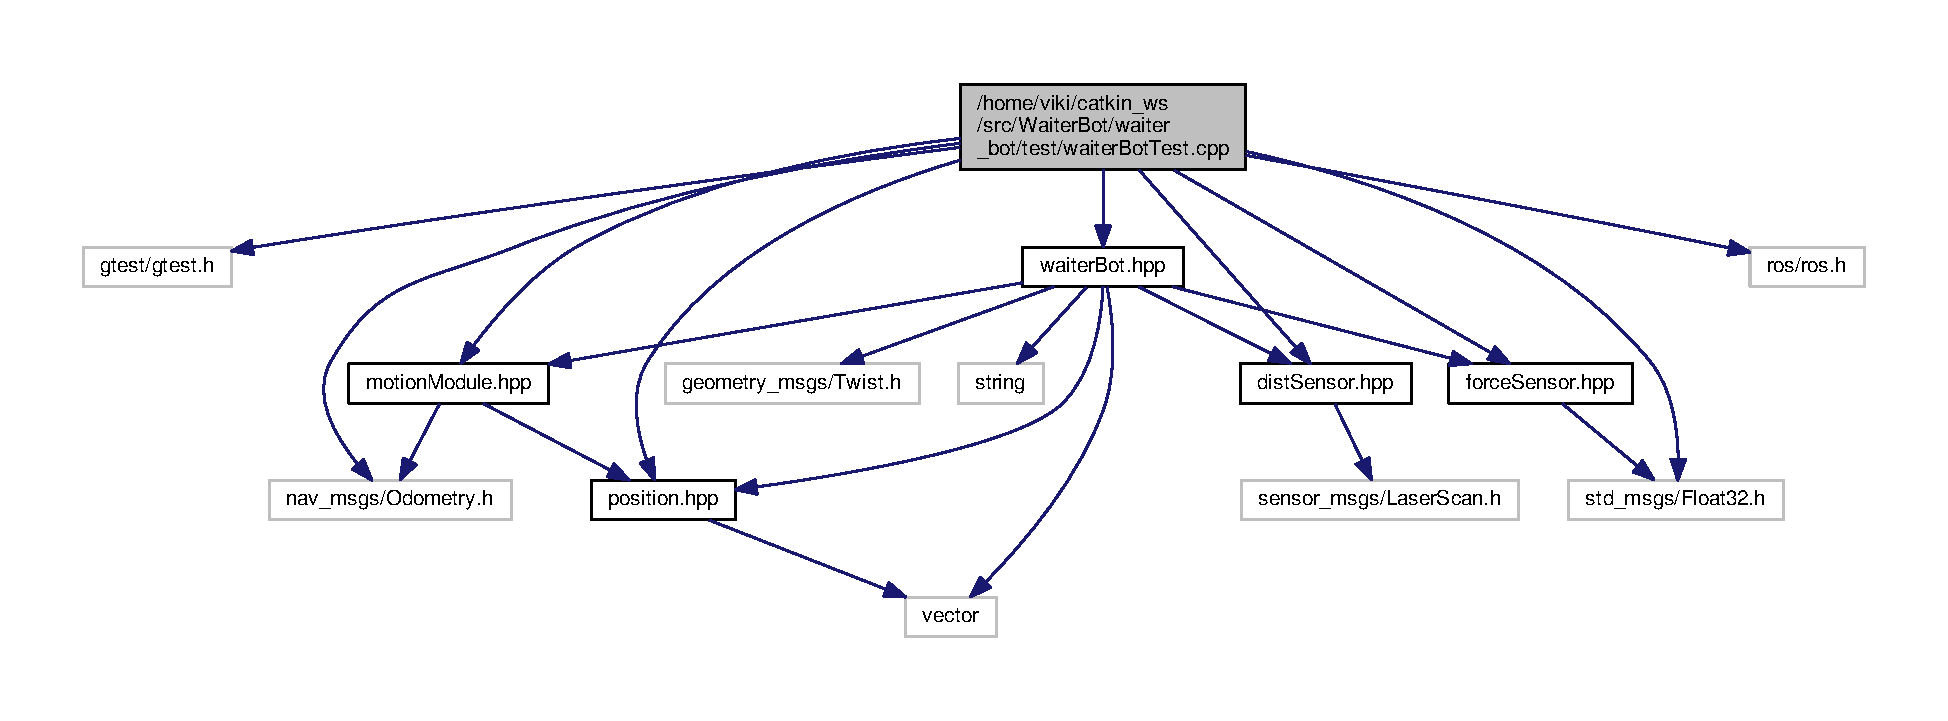
\includegraphics[width=350pt]{waiterBotTest_8cpp__incl}
\end{center}
\end{figure}
\subsection*{Functions}
\begin{DoxyCompactItemize}
\item 
\hyperlink{waiterBotTest_8cpp_adc7b03a710ceadf182f21551e58e5cd8}{T\+E\+ST} (waiter\+Bot\+Test, constructor\+Test)
\begin{DoxyCompactList}\small\item\em test the \hyperlink{classwaiterBot}{waiter\+Bot} constructor \end{DoxyCompactList}\item 
\hyperlink{waiterBotTest_8cpp_a7026628c90cebc2b041a91c1875b6721}{T\+E\+ST} (waiter\+Bot\+Test, get\+Angle\+Diff\+Test)
\begin{DoxyCompactList}\small\item\em test the get\+Angle\+Diff funtion \end{DoxyCompactList}\item 
\hyperlink{waiterBotTest_8cpp_a37b09c0b5a5b3d3b062e46a2be1da656}{T\+E\+ST} (waiter\+Bot\+Test, move\+Stop\+Test)
\begin{DoxyCompactList}\small\item\em test the stop section of the move funtion \end{DoxyCompactList}\item 
\hyperlink{waiterBotTest_8cpp_a1ee3b0f440490f75f86e6dbb388c1821}{T\+E\+ST} (waiter\+Bot\+Test, move\+No\+Food\+Test)
\begin{DoxyCompactList}\small\item\em test the no food section of the move funtion \end{DoxyCompactList}\item 
\hyperlink{waiterBotTest_8cpp_a71ef0d18bc3937aa2d63faa698f82cb1}{T\+E\+ST} (waiter\+Bot\+Test, move\+In\+Target\+Location\+Test)
\begin{DoxyCompactList}\small\item\em test the in target location section of the move funtion \end{DoxyCompactList}\end{DoxyCompactItemize}


\subsection{Detailed Description}
This is the \char`\"{}.\+cpp\char`\"{} file for testing the \hyperlink{classwaiterBot}{waiter\+Bot} class. 

\begin{DoxyAuthor}{Author}
Ruben Acevedo
\end{DoxyAuthor}
\begin{DoxyCopyright}{Copyright}
\mbox{[}2017\mbox{]} Ruben Acevedo 
\end{DoxyCopyright}


\subsection{Function Documentation}
\index{waiter\+Bot\+Test.\+cpp@{waiter\+Bot\+Test.\+cpp}!T\+E\+ST@{T\+E\+ST}}
\index{T\+E\+ST@{T\+E\+ST}!waiter\+Bot\+Test.\+cpp@{waiter\+Bot\+Test.\+cpp}}
\subsubsection[{\texorpdfstring{T\+E\+S\+T(waiter\+Bot\+Test, constructor\+Test)}{TEST(waiterBotTest, constructorTest)}}]{\setlength{\rightskip}{0pt plus 5cm}T\+E\+ST (
\begin{DoxyParamCaption}
\item[{waiter\+Bot\+Test}]{, }
\item[{constructor\+Test}]{}
\end{DoxyParamCaption}
)}\hypertarget{waiterBotTest_8cpp_adc7b03a710ceadf182f21551e58e5cd8}{}\label{waiterBotTest_8cpp_adc7b03a710ceadf182f21551e58e5cd8}


test the \hyperlink{classwaiterBot}{waiter\+Bot} constructor 

M\+IT License

Copyright 2017 Ruben Acevedo

Permission is hereby granted, free of charge, to any person obtaining a copy of this software and associated documentation files (the \char`\"{}\+Software\char`\"{}), to deal in the Software without restriction, including without limitation the rights to use, copy, modify, merge, publish, distribute, sublicense, and/or sell copies of the Software, and to permit persons to whom the Software is furnished to do so, subject to the following conditions\+:

The above copyright notice and this permission notice shall be included in all copies or substantial portions of the Software. T\+HE S\+O\+F\+T\+W\+A\+RE IS P\+R\+O\+V\+I\+D\+ED \char`\"{}\+A\+S I\+S\char`\"{}, W\+I\+T\+H\+O\+UT W\+A\+R\+R\+A\+N\+TY OF A\+NY K\+I\+ND, E\+X\+P\+R\+E\+SS OR I\+M\+P\+L\+I\+ED, I\+N\+C\+L\+U\+D\+I\+NG B\+UT N\+OT L\+I\+M\+I\+T\+ED TO T\+HE W\+A\+R\+R\+A\+N\+T\+I\+ES OF M\+E\+R\+C\+H\+A\+N\+T\+A\+B\+I\+L\+I\+TY, F\+I\+T\+N\+E\+SS F\+OR A P\+A\+R\+T\+I\+C\+U\+L\+AR P\+U\+R\+P\+O\+SE A\+ND N\+O\+N\+I\+N\+F\+R\+I\+N\+G\+E\+M\+E\+NT. IN NO E\+V\+E\+NT S\+H\+A\+LL T\+HE A\+U\+T\+H\+O\+RS OR C\+O\+P\+Y\+R\+I\+G\+HT H\+O\+L\+D\+E\+RS BE L\+I\+A\+B\+LE F\+OR A\+NY C\+L\+A\+IM, D\+A\+M\+A\+G\+ES OR O\+T\+H\+ER L\+I\+A\+B\+I\+L\+I\+TY, W\+H\+E\+T\+H\+ER IN AN A\+C\+T\+I\+ON OF C\+O\+N\+T\+R\+A\+CT, T\+O\+RT OR O\+T\+H\+E\+R\+W\+I\+SE, A\+R\+I\+S\+I\+NG F\+R\+OM, O\+UT OF OR IN C\+O\+N\+N\+E\+C\+T\+I\+ON W\+I\+TH T\+HE S\+O\+F\+T\+W\+A\+RE OR T\+HE U\+SE OR O\+T\+H\+ER D\+E\+A\+L\+I\+N\+GS IN T\+HE S\+O\+F\+T\+W\+A\+RE. © 2017 Git\+Hub, Inc. This tests makes sure that the constructor works It should set the target locations to be (0,0) (10,0) (10,10) (10,0) It should set the status to \char`\"{}in target location 1\char`\"{} It should set the stopB to false; It also test the get\+Target\+Locs() and get\+Status() did\+Stop() at the same time \index{waiter\+Bot\+Test.\+cpp@{waiter\+Bot\+Test.\+cpp}!T\+E\+ST@{T\+E\+ST}}
\index{T\+E\+ST@{T\+E\+ST}!waiter\+Bot\+Test.\+cpp@{waiter\+Bot\+Test.\+cpp}}
\subsubsection[{\texorpdfstring{T\+E\+S\+T(waiter\+Bot\+Test, get\+Angle\+Diff\+Test)}{TEST(waiterBotTest, getAngleDiffTest)}}]{\setlength{\rightskip}{0pt plus 5cm}T\+E\+ST (
\begin{DoxyParamCaption}
\item[{waiter\+Bot\+Test}]{, }
\item[{get\+Angle\+Diff\+Test}]{}
\end{DoxyParamCaption}
)}\hypertarget{waiterBotTest_8cpp_a7026628c90cebc2b041a91c1875b6721}{}\label{waiterBotTest_8cpp_a7026628c90cebc2b041a91c1875b6721}


test the get\+Angle\+Diff funtion 

This tests makes sure its returns the angle difference correctly Given a location it should say how much you need to turn in radians to head straight for that location. Tests 9 differnt locations in all 4 quadrants \index{waiter\+Bot\+Test.\+cpp@{waiter\+Bot\+Test.\+cpp}!T\+E\+ST@{T\+E\+ST}}
\index{T\+E\+ST@{T\+E\+ST}!waiter\+Bot\+Test.\+cpp@{waiter\+Bot\+Test.\+cpp}}
\subsubsection[{\texorpdfstring{T\+E\+S\+T(waiter\+Bot\+Test, move\+Stop\+Test)}{TEST(waiterBotTest, moveStopTest)}}]{\setlength{\rightskip}{0pt plus 5cm}T\+E\+ST (
\begin{DoxyParamCaption}
\item[{waiter\+Bot\+Test}]{, }
\item[{move\+Stop\+Test}]{}
\end{DoxyParamCaption}
)}\hypertarget{waiterBotTest_8cpp_a37b09c0b5a5b3d3b062e46a2be1da656}{}\label{waiterBotTest_8cpp_a37b09c0b5a5b3d3b062e46a2be1da656}


test the stop section of the move funtion 

This tests the stop sections of code in the move function If the \hyperlink{classdistSensor}{dist\+Sensor} says it is in collision the robot should stop Get collision data\index{waiter\+Bot\+Test.\+cpp@{waiter\+Bot\+Test.\+cpp}!T\+E\+ST@{T\+E\+ST}}
\index{T\+E\+ST@{T\+E\+ST}!waiter\+Bot\+Test.\+cpp@{waiter\+Bot\+Test.\+cpp}}
\subsubsection[{\texorpdfstring{T\+E\+S\+T(waiter\+Bot\+Test, move\+No\+Food\+Test)}{TEST(waiterBotTest, moveNoFoodTest)}}]{\setlength{\rightskip}{0pt plus 5cm}T\+E\+ST (
\begin{DoxyParamCaption}
\item[{waiter\+Bot\+Test}]{, }
\item[{move\+No\+Food\+Test}]{}
\end{DoxyParamCaption}
)}\hypertarget{waiterBotTest_8cpp_a1ee3b0f440490f75f86e6dbb388c1821}{}\label{waiterBotTest_8cpp_a1ee3b0f440490f75f86e6dbb388c1821}


test the no food section of the move funtion 

This tests the no food sections of code in the move function If the \hyperlink{classforceSensor}{force\+Sensor} states that there is no food then the robot should change its status to heading to location 1 setting force message to be 0

place robot not in location 1 since here it can never not have food\index{waiter\+Bot\+Test.\+cpp@{waiter\+Bot\+Test.\+cpp}!T\+E\+ST@{T\+E\+ST}}
\index{T\+E\+ST@{T\+E\+ST}!waiter\+Bot\+Test.\+cpp@{waiter\+Bot\+Test.\+cpp}}
\subsubsection[{\texorpdfstring{T\+E\+S\+T(waiter\+Bot\+Test, move\+In\+Target\+Location\+Test)}{TEST(waiterBotTest, moveInTargetLocationTest)}}]{\setlength{\rightskip}{0pt plus 5cm}T\+E\+ST (
\begin{DoxyParamCaption}
\item[{waiter\+Bot\+Test}]{, }
\item[{move\+In\+Target\+Location\+Test}]{}
\end{DoxyParamCaption}
)}\hypertarget{waiterBotTest_8cpp_a71ef0d18bc3937aa2d63faa698f82cb1}{}\label{waiterBotTest_8cpp_a71ef0d18bc3937aa2d63faa698f82cb1}


test the in target location section of the move funtion 

This tests the in target location sections of code in the move function If the robot gets to a target location it changes its status to \char`\"{}in target location \#\char`\"{} If the robot has already been marked as being in that specific target location it sets its status to move to the next location place robot in location 2

place robot in location 3

place robot in location 4

place robot in location 1
%--- End generated contents ---

% Index
\backmatter
\newpage
\phantomsection
\clearemptydoublepage
\addcontentsline{toc}{chapter}{Index}
\printindex

\end{document}
